\documentclass[12pt,a4paper,oneside]{book}

\usepackage{mglthesis}

\def\ucllogoontitlepage{1}

%% % Golden ratio for the textblock. A4 is 210mm x 297mm. (297 - 35 - 35)
%% % / (210 - 40 - 30) is about 1.618. 80 characters per line. 36 lines
%% % with 18pt baselineskip.
%% \usepackage[inner=40mm,outer=30mm,top=35mm,bottom=35mm,
%%   headheight=20mm,marginparwidth=20mm]{geometry}

% Left margin: 1/5 of width, right margin: 1/6. 75 characters per
% line. Visual top margin (to the midline of the top line) is equal to
% the left margin. Bottom margin is random. Text block is golden
% ratio.

%% % 35 lines with 18pt baselineskip.
%% \usepackage[inner=42mm,outer=35mm,top=37.77mm,bottom=38.1mm,
%%   headheight=20mm,marginparwidth=20mm,footskip=32pt]{geometry}

%% % 36 lines with 17.5pt baselineskip.
%% \usepackage[inner=42mm,outer=35mm,top=37.77mm,bottom=38.1mm,
%%   headheight=20mm,marginparwidth=20mm,footskip=31pt]{geometry}

%% % 37 lines with 17pt baselineskip.
%% \usepackage[inner=42mm,outer=35mm,top=37.77mm,bottom=39.0mm,
%%   headheight=20mm,marginparwidth=20mm,footskip=32pt]{geometry}

%% % 38 lines with 16.5pt baselineskip.
%% \usepackage[inner=42mm,outer=35mm,top=37.77mm,bottom=39.7mm,
%%   headheight=20mm,marginparwidth=20mm,footskip=31pt]{geometry}

% 38 lines with 16.2pt baselineskip (3*x-height, which is 5.4pt).
\usepackage[inner=42mm,outer=35mm,top=37.77mm,bottom=37.5mm,
  headheight=20mm,marginparwidth=20mm,footskip=31pt]{geometry}

\usepackage{eso-pic}

\makeatletter
\newcommand*\currentfontsize{\dimexpr\f@size pt\relax}
\makeatother

\onehalfspacing

\ifxetex
  \usepackage{xintexpr}
  \renewcommand{\textls}[2][0]
               {{\addfontfeature{LetterSpace=\xinttheexpr0.1*#1\relax}#2}}
\fi
\ifluatex
  \usepackage{xintexpr}
  \renewcommand{\textls}[2][0]
               {{\addfontfeature{LetterSpace=\xinttheexpr0.1*#1\relax}#2}}
\fi


%%%% Title page

\usepackage{svg}
\usepackage{anyfontsize}
\usepackage{color}
\usepackage{xcolor}
\definecolor{ucllogocolor}{RGB}{35,31,32}
\definecolor{titlepagefg}{RGB}{229,225,226}
\definecolor{mglred}{RGB}{163,65,48}
\definecolor{mglgreen}{RGB}{37,125,49}
\definecolor{mglblue}{RGB}{65,48,163}
\definecolor{mglred2}{RGB}{131,51,39}
\definecolor{mglredsmall}{RGB}{180,45,25}


%%%% Math

\usepackage{bbm}
\usepackage{thmtools}
\usepackage{thm-restate}
\usepackage{nicefrac}
\usepackage{centernot}
\allowdisplaybreaks


%%%% Floats (Tables, Figures, Algorithms)

\usepackage[font=small]{caption}
\usepackage{subcaption}
\usepackage{booktabs}
\usepackage{multirow}
\usepackage{siunitx}
\sisetup{detect-all}
\usepackage[noend]{algpseudocode}
\usepackage{algorithm,algorithmicx}
\newcommand*\Let[2]{\State #1 $\gets$ #2}
\usepackage{tabularx}
\usepackage{graphicx}
\usepackage{float}
\renewcommand{\floatpagefraction}{.8}
% https://tex.stackexchange.com/questions/28556/how-to-place-a-float-at-the-top-of-a-floats-only-page
\makeatletter
\setlength{\@fptop}{0pt}
\setlength{\@fpbot}{0pt plus 50fil}
\makeatother


%%%% Misc

\usepackage{xspace}
\usepackage{marvosym}


%%%% Tikz and Pgfplots

\usepackage{tikz}
\usepackage{pgfplots,tikz,pgfplotstable}
\pgfplotsset{compat=1.9}
\usetikzlibrary{positioning, fit, arrows.meta, shapes}
\usetikzlibrary{external}
\tikzexternalize[prefix=tikz/]
\tikzset{external/optimize command away=\AddToShipoutPictureBG}

% https://tex.stackexchange.com/questions/84127/correctly-align-vertical-text-on-a-baseline-in-pgfplots
\def\mystrut{\vphantom{hg}}
% https://tex.stackexchange.com/questions/204395/add-custom-entry-into-legend-in-pgfplot
\pgfplotsset{
    legend image with text/.style={
        legend image code/.code={%
            \node[anchor=center] at (0.3cm,0cm) {#1};
        }
    },
}
\pgfplotsset{%
  redweak/.style = {red!70!black,densely dotted,
                    mark=o, mark options={scale=0.7,solid}}}
\pgfplotsset{%
  redhollow/.style = {red!100!white,densely dashed,
                      mark=o, mark options={scale=1.0,solid}}}
\pgfplotsset{%
  redsolid/.style = {red!50!white,mark=*,mark options={scale=1.0,solid}}}

\pgfplotsset{%
  orangeweak/.style = {orange!70!black,densely dotted,mark=diamond,
                       mark options={scale=1.2*0.7,solid}}}
\pgfplotsset{%
  orangehollow/.style = {orange!100!white,densely dashed,mark=diamond,
                         mark options={scale=1.2,solid}}}
\pgfplotsset{%
  orangesolid/.style = {orange!50!white,mark=diamond*,
                        mark options={scale=1.2,solid}}}

\pgfplotsset{%
  violetweak/.style = {violet!70!black,densely dotted,mark=diamond,
                       mark options={scale=1.2*0.7,solid}}}
\pgfplotsset{%
  violethollow/.style = {violet!100!white,densely dashed,mark=diamond,
                         mark options={scale=1.2,solid}}}
\pgfplotsset{%
  violetsolid/.style = {violet!50!white,mark=diamond*,
                        mark options={scale=1.2,solid}}}

\pgfplotsset{%
  blueweak/.style = {blue!70!black,densely dotted,mark=square,
                     mark options={scale=0.8*0.7,solid}}}
\pgfplotsset{%
  bluehollow/.style = {blue!100!white,densely dashed,mark=square,
                       mark options={scale=0.8,solid}}}
\pgfplotsset{%
  bluesolid/.style = {blue!50!white,mark=square*,
                      mark options={scale=0.8,solid}}}

\pgfplotsset{%
  tealweak/.style = {teal!70!black,densely dotted,mark=triangle,
                     mark options={scale=1.2*0.7,solid}}}
\pgfplotsset{%
  tealhollow/.style = {teal!100!white,densely dashed,mark=triangle,
                       mark options={scale=1.2,solid}}}
\pgfplotsset{%
  tealsolid/.style = {teal!50!white,mark=triangle*,
                      mark options={scale=1.2,solid}}}

\newcommand*\circled[2]{\tikz[baseline=(char.base)]{
    \node[shape=circle,draw,inner sep=#2pt] (char) {#1};}}

\pgfplotscreateplotcyclelist{acycle}{%
solid, every mark/.append style={solid, fill=gray}, mark=*\\%
dotted, every mark/.append style={solid, fill=gray}, mark=square*\\%
densely dotted, every mark/.append style={solid, fill=gray}, mark=otimes*\\%
loosely dotted, every mark/.append style={solid, fill=gray}, mark=triangle*\\%
dashed, every mark/.append style={solid, fill=gray},mark=diamond*\\%
loosely dashed, every mark/.append style={solid, fill=gray},mark=*\\%
densely dashed, every mark/.append style={solid, fill=gray},mark=square*\\%
dashdotted, every mark/.append style={solid, fill=gray},mark=otimes*\\%
dashdotdotted, every mark/.append style={solid},mark=star\\%
densely dashdotted,every mark/.append style={solid, fill=gray},mark=diamond*\\%
}


%%%% New environments, commands

%% \newtheoremstyle{mglthm}
%%                 {\baselineskip}% Space above
%%                 {\baselineskip}% Space below
%%                 {\itshape}% Body font
%%                 {}% Indent amount
%%                 {\bfseries}% Theorem head font
%%                 {:}% Punctuation after theorem head
%%                 {.5em}% Space after theorem head
%%                 {}% Theorem head spec (can be left empty, meaning ‘normal’)
%% \theoremstyle{mglthm}

\newtheorem{definition}{Definition}
\newtheorem{theorem}{Theorem}
\newtheorem{proposition}[theorem]{Proposition}
\newtheorem{corollary}[theorem]{Corollary}
\newtheorem{lemma}[theorem]{Lemma}
\newtheorem{assumption}{Assumption}

\newcommand\numberthis{\addtocounter{equation}{1}\tag{\theequation}}

%% Use slanted leq and geq by default.
\let\savedleq=\leq
\let\savedgeq=\geq
\let\leq=\leqslant
\let\geq=\geqslant

\DeclareMathOperator*{\argmin}{arg\,min}
\DeclareMathOperator*{\argmax}{arg\,max}
\DeclareMathOperator*{\softmax}{softmax}
\DeclarePairedDelimiter{\ceil}{\lceil}{\rceil}
\DeclarePairedDelimiter{\floor}{\lfloor}{\rfloor}
\DeclarePairedDelimiter{\norm}{\lVert}{\rVert}
\DeclarePairedDelimiter{\abs}{\lvert}{\rvert}
\DeclareMathOperator*{\diag}{diag}

%% % https://tex.stackexchange.com/questions/29834/closed-square-root-symbol
%% % The magic numbers are font specific.
%% \let\oldsqrt\sqrt
%% \def\sqrt{\mathpalette\DHLhksqrt}
%% \def\DHLhksqrt#1#2{%
%% \setbox0=\hbox{$#1\oldsqrt{#2}$}\dimen0=\ht0
%% \advance\dimen0-0.2\ht0
%% \setbox2=\hbox{\vrule height\ht0 depth -\dimen0 width 0.66pt}%
%% {\box0\lower0.66pt\box2}}

%% Like overset but uses less vertical space.
\makeatletter
\newcommand{\oset}[3][0ex]{%
  \mathrel{\mathop{#3}\limits^{
    \vbox to#1{\kern-3\ex@
    \hbox{$\scriptstyle#2$}\vss}}}}
\makeatother
\newcommand{\pto}{\oset{p}\to}

%% \newcommand\dif{\mathop{}\!d}
\newcommand\dif{\,d}
\newcommand{\Loss}{\mathcal{L}}
\newcommand{\N}{\mathcal{N}}
\newcommand{\Nb}{\mathbb{N}}
\newcommand{\Rb}{\mathbb{R}}
\newcommand{\I}{\mathrm{I}}
\newcommand{\ind}{\mathbb{I}}
\newcommand{\indcia}{\mathbbm{1}_{[1,k]}(i)z}
\newcommand{\E}{\mathop{{}\mathbb{E}}}
% Reduce the space around | in p(x \mid y)
\newcommand{\tmid}{\hspace{0.08em}|\hspace{0.11em}}
\newcommand{\divides}{\mathrel{|}}
\DeclarePairedDelimiterX{\condp}[2]{(}{)}{%
  #1\;\delimsize|\penalty 0 \;#2%
}
\DeclareMathOperator{\KL}{KL}
\DeclarePairedDelimiterX{\infdivx}[2]{(}{)}{%
  #1\;\delimsize\|\penalty 0 \;#2%
}
\newcommand{\Div}{\infdivx}
\DeclareMathOperator{\var}{var}
\DeclareMathOperator\supp{supp}
\DeclareMathOperator{\elbo}{\mathrm{ELBO}}
\newcommand{\w}{\omega}
\newcommand{\vw}{\mathbf{w}}
\newcommand{\vx}{\mathbf{x}}
\newcommand{\vc}{\mathbf{c}}
\newcommand{\vh}{\mathbf{h}}
\newcommand{\vy}{\mathbf{y}}
\newcommand{\vb}{\mathbf{b}}
\newcommand{\vf}{\mathbf{f}}
\newcommand{\vi}{\mathbf{i}}
\newcommand{\vj}{\mathbf{j}}
\newcommand{\vo}{\mathbf{o}}
\newcommand{\va}{\mathbf{a}}
\newcommand{\vu}{\mathbf{u}}
\newcommand{\vecv}{\mathbf{v}}
\newcommand{\vcprev}{\mathbf{c}_{\textit{prev}}}
\newcommand{\vhprev}{\mathbf{h}_{\textit{prev}}}
\newcommand{\mA}{\mathbf{A}}
\newcommand{\mX}{\mathbf{X}}
\newcommand{\mW}{\mathbf{W}}
\newcommand{\mQ}{\mathbf{Q}}
\newcommand{\mR}{\mathbf{R}}
\newcommand{\mE}{\mathbf{E}}
\newcommand{\mM}{\mathbf{M}}
\newcommand{\OL}{\Delta}
\newcommand{\dotinnode}{\raisebox{-4pt}{$\cdot$}}
\DeclareMathOperator*{\LSTM}{LSTM}
\DeclareMathOperator*{\mLSTM}{mLSTM}
\DeclareMathOperator*{\RLSTM}{RLSTM}
\DeclareMathOperator*{\mogrify}{mogrify}
\DeclareMathOperator*{\Mogrify}{Mogrify}
\DeclareMathOperator*{\onehot}{onehot}
\DeclareMathOperator*{\dec}{dec}
%% \DeclareMathOperator*{\tanh}{tanh}
\newcommand{\Lim}[1]{\raisebox{0.5ex}{\scalebox{1.0}{$\displaystyle \lim_{#1}\;$}}}
\newcommand{\indep}{\perp \!\!\! \perp}
\newcommand{\notindep}{\not\!\perp\!\!\!\perp}

\newcommand{\tta}{\textlf{2}TA}

\newcommand*{\circledtiny}[2]{\raisebox{0.2ex}{\circled{\tiny#1}{#2}}}
\newcommand{\smallsharp}{\scalebox{0.6}{\raisebox{0.2ex}{$\sharp$}}}
\newcommand{\hardposteriorcircled}{%
  \raisebox{0.2ex}{\circled{$\smallsharp$}{0.8}}}
\newcommand{\expansioncircled}{%
  \raisebox{0.1ex}{\circled{\small$\times$}{-0.5}}}
\newcommand{\equalcircled}{%
  \raisebox{1.0ex}{\circled{\raisebox{-0.7ex}{\tiny$=$}}{0.5}}}

\newcommand{\alphanorm}{{\bar{\alpha}}}
\newcommand{\raisedcomma}{\raisebox{0.5ex}{$,$}}
\newcommand{\alphasharp}{{\alpha\smallsharp}}
\newcommand{\alphajoint}{{\alpha\raisedcomma}}
\newcommand{\alphacond}{{\alpha|}}
\newcommand{\alpharange}{{1:\alpha}}
\newcommand{\xalpha}{{x_\alpharange}}
\newcommand{\calpha}{{\ceil{\alpha}}}
\newcommand{\calpharange}{{1:\calpha}}
\newcommand{\xcalpha}{{x_\calpharange}}

\newcommand{\ptb}{PTB\xspace}
\newcommand{\wikitexttwo}{Wikitext-$2$\xspace}
\newcommand{\enwik}{Enwik8\xspace}
\newcommand{\texteight}{Text8\xspace}
\newcommand{\nlltoppl}[1]{%
  \pgfmathparse{exp(#1)}%
  \pgfmathprintnumber[fixed,zerofill,precision=1,assume math mode=true]{\pgfmathresult}}
\newcommand{\nlltopplbold}[1]{%
  \pgfmathparse{exp(#1)}%
  \textbf{\pgfmathprintnumber[fixed,zerofill,precision=1,assume math mode=true]{\pgfmathresult}}}
\newcommand{\nlltobpc}[1]{%
  \pgfmathparse{log2(exp(#1))}%
  \pgfmathprintnumber[fixed,zerofill,precision=3,assume math mode=true]{\pgfmathresult}}
\newcommand{\nlltobpcbold}[1]{%
  \pgfmathparse{log2(exp(#1))}%
  \textbf{\pgfmathprintnumber[fixed,zerofill,precision=3,assume math mode=true]{\pgfmathresult}}}

\newcommand{\betavae}{$\upbeta$-VAE\xspace}
\newcommand{\cX}{\mathcal{X}}

\DeclareMathOperator*{\avg}{avg}
\newcommand*{\SP}{\mathrm{SP}}
\newcommand*{\natnum}{\mathbb{N}}
\newcommand*{\natnumzero}{\mathbb{N}_0}

\newcommand\ts{\hspace{0.2em}/\hspace{0.2em}}


%%%% Todolist

\usepackage{xargs} % Use more than one optional parameter in new commands
\usepackage[colorinlistoftodos,prependcaption,textsize=tiny]{todonotes}

\makeatletter
\renewcommand{\todo}[2][]{\tikzexternaldisable\@todo[#1]{#2}\tikzexternalenable}
\newcommand\nobreakpar{\par\nobreak\@afterheading}
\makeatother

% colorbox with no margins
\newcommand{\reducedstrut}{\vrule width 0pt height .9\ht\strutbox depth .9\dp\strutbox\relax}
\newcommand{\colorboxx}[2]{%
  \begingroup%
  \setlength{\fboxsep}{0pt}%
  \colorbox{#1}{\reducedstrut#2\/}%
  \endgroup
}
\newcommandx{\mgl}[2][1=]{\colorboxx{blue!30}{\tiny\,}\todo[color=blue!30,#1]{MG: #2}}
\newcommandx{\tk}[2][1=]{\colorboxx{brown!30}{\tiny\,}\todo[color=brown!30,#1]{TK: #2}}
\newcommandx{\pb}[2][1=]{\colorboxx{gray!30}{\tiny\,}\todo[color=gray!30,#1]{PB: #2}}
\newcommandx{\cd}[2][1=]{\colorboxx{cyan!30}{\tiny\,}\todo[color=cyan!30,#1]{CD: #2}}
\newcommandx{\jr}[2][1=]{\colorboxx{red!30}{\tiny\,}\todo[color=red!30,#1]{JR: #2}}
\newcommand{\inlinetodo}[1]{\textcolor{blue}{\bf \small #1}}


\begin{document}

\begin{titlepage}
  % Line right edge up the the L of the UCL logo.
  \newgeometry{inner=47mm,outer=31mm,bottom=20mm}
  \AddToShipoutPictureBG*{%
    \AtPageLowerLeft{%
      \color{titlepagefg}
      \rule{\paperwidth}{\paperheight}%
    }%
    \ifnum \ucllogoontitlepage = 0
      \AtPageUpperLeft{%
        \color{ucllogocolor}%
        \rule[-\paperheight]{\paperwidth}{\paperheight}%
      }%
    \else%
      \AtPageLowerLeft{%
        \includesvg[width=\paperwidth]{ucl.svg}
      }%
      \AtPageUpperLeft{%
        \color{ucllogocolor}%
        \rule[-0.8\paperheight]{\paperwidth}{0.81\paperheight}%
      }%
    \fi%
  }%
  \color{titlepagefg}
  \setstretch{1.0}
  \begin{flushleft}
    % 12.115pt is the visual x-height with 25pt EB Garamond.
    % 17.759pt is the visual cap height with 25pt EB Garamond.
    % 4*12.115pt=48.46pt
    % the title page.
    {\fontsize{25pt}{48.46pt}
      \sc\titlefont\textls[100]{\\[-32pt]
      Towards\, Better\\
      Generative\, Models\\
      {\fontsize{23pt}{48.46pt}\selectfont\textls[0]{%
        \hbox to 0pt{\hss \textup{\textit{of}}\:}}}%
      Language\\}}
    % 5*12.115pt=60.575pt
    {\fontsize{23pt}{60.575pt}\titlefont
      \color{mglred}
      \textit{Gábor Melis}\\}
  \end{flushleft}
  \begin{flushright}
    \ifnum \ucllogoontitlepage = 0
      \vspace{121.15pt+48.46pt}
    \else
      \vspace{121.15pt}
    \fi
    % This line spread is the same as above, but the font size is such
    % that the leading is 2*12.115pt=24.23pt.
    {\fontsize{12.5pt}{24.23pt}\titlefont
      A thesis presented for the degree of\\
      Doctor of Philosophy\\[0.5\baselineskip]
      % 11.5pt/12.5 = 23pt/25pt
      {\fontsize{11.5pt}{24.23pt}\textit{at the}}\\[0.5\baselineskip]
%%     {\large Centre for Mathematics, Physics and Engineering \\
%%       in the Life Sciences and Experimental Biology\\
%%       University College London,\\
%%       United Kingdom\\}
      Computer Science Department,\\
      University College London,\\
      United Kingdom\\[1\baselineskip]
      {\fontsize{11.5pt}{24.23pt}\textit{April, 2023}}}
  \end{flushright}
\end{titlepage}

\begin{titlepage}
\vspace*{16\groundskip}
\noindent I, Gábor Melis, confirm that the work presented in this thesis is my own.
Where information has been derived from other sources, I confirm that this has been indicated in the thesis.
\end{titlepage}

% UCL says that page 1 must be the title page.
\setcounter{page}{3}

\chapter*{Abstract}

\mglepigraph{0.6}{A man who could afford fifty dollars had a pair of boots that'd still be keeping his feet dry in ten years' time, while the poor man who could only afford cheap boots would have spent a hundred dollars on boots in the same time and would still have wet feet.}%
            {Capt. Samuel Vimes}
\mgllettrine{findent=-1.2em,nindent=0.8em,slope=0.9em}{A}{s language}
modelling has been progressing immensely towards genuinely useful applications driven by the increased availability of data and computational resources, our understanding and tools have not kept pace.
On the one hand, it  is usual for understanding to lag behind practice; on the other, often a steep price is to be paid for letting practice race too far ahead.
A trained language model is the product of the interactions of data, optimization, the training objective, regularization, and the model itself, which not only provide rich veins for research individually but combine to create significant complexity, which hampers progress.
This thesis pursues advances along these directions to solidify the footing and our understanding of the model and the process of its training in hopes of guiding research and applications towards better solutions.


\chapter*{Impact Statement}

\mglepigraph{0.46}{We don't measure our success by results but by activity, and the activity is considerable and productive.}{Sir Humphrey Appleby}
\mgllettrine{lhang=0.05,findent=-0.3em,nindent=0.5em}{G}{oals and contributions}
of this thesis include designing better recurrent neural networks and new methods of optimization as well as inference in latent variable models, with a focus on advancing language models.
Recurrent neural networks are state-of-the-art models in small-scale language modelling and various other domains.
We improve them even further, which has the most direct impact on machine learning practitioners.
Ironically, the practice of language modelling is currently dominated by attention-based models due to their scalability, optimizability and the importance of training on large amounts of data.
Can recurrent models match them with enough resources?
We take a small step towards answering this question by scaling recurrent models with the help of our proposed optimization algorithm.
We demonstrate that the improved recurrent models are capable of matching attention-based models on bigger --~but still tiny by today's standards~-- datasets.
Finding that the gap between these models is not nearly as large as previously believed, we turn our attention to other ways of improvement.
We hope to inject structure and useful biases into the model with conditional independence assumptions and the shaping of the latent space, but posterior collapse gets in the way.
To address this, we introduce a new inference method for latent variable models, opening the door for this class of generative models to be used successfully in practice.
While the focus of this thesis is very specific, all of our contributions are applicable beyond language modelling.


\chapter*{Acknowledgements}

First and foremost, I would like to thank my supervisors, Phil Blunsom, Chris Dyer, and Thore Graepel, for instilling a coherent, deeply probabilistic worldview in me, for letting me find my own way in research but guiding me through the PhD process.
I thank DeepMind for being a great working environment for so long and for sponsoring my studies at UCL.
I am especially grateful to my collaborators and colleagues over the years, who furnished me with insight, valuable feedback, and the Oxford comma.\\

\noindent
\textit{Végül, de nem utolsósorban, köszönöm szűkebb családomnak a bíztatást, hogy a doktorit kezdjem el, majd hogy fejezzem be.
Legvégül talán köszönöttel tartozom azoknak, akik értékeiket belém plántálták, és egész biztosan hálával azoknak, akik megértésükkel, támogatásukkal, tudásukkal segítettek: szüleimnek, Hernádi Zsuzsa tanárnőnek, és a Toldy Ferenc gimnázium tanárainak.}


%% %% This chapter is for the official submission only.
%% \chapter*{UCL Research Paper Declaration}
%% 
%% \begin{enumerate}
%% \item \textbf{Published manuscript}
%%   \begin{itemize}
%%   \item \textbf{Title:} Mogrifier LSTM
%%   \item \textbf{Link:} \url{https://openreview.net/forum?id=SJe5P6EYvS}
%%   \item \textbf{Published at:} ICLR
%%   \item \textbf{Published by:} OpenReview
%%   \item \textbf{Publishing date:} 2020
%%   \item \textbf{Authors:} Gábor Melis, Tom{\'a}{\v{s}} Ko{\v{c}}isk{\`y}, Phil Blunsom
%%   \item \textbf{Peer reviewed?} Yes
%%   \item \textbf{Have you retained the copyright?} Yes
%%   \item \textbf{Preprint:} \url{https://arxiv.org/abs/1909.01792}.
%%   \item \textbf{Statement of contribution of all authors:}
%%     I did most of the work; my coauthors suggested experiments and provided feedback.
%%   \item \textbf{Thesis chapter:} \Cref{sec:timid-transformation}
%%   \item \textbf{E-signatures confirming that the information above is accurate}
%%     \begin{ground}
%%       \vspace{12pt}
%%       \hspace{4em}\includegraphics[width=0.8\textwidth]{figure/signature1.png}
%%     \end{ground}
%%   \end{itemize}
%% \clearpage
%% 
%% \item \textbf{Unpublished manuscript}
%%   \begin{itemize}
%%   \item \textbf{Title:} Two-Tailed Averaging: Anytime, Adaptive, Once-in-a-While Optimal Weight Averaging for Better Generalization
%%   \item \textbf{Preprint:} \url{https://arxiv.org/abs/2209.12581}
%%   \item \textbf{To be published at:} Not decided
%%   \item \textbf{Authors:} Gábor Melis
%%   \item \textbf{Stage of publication:} None
%%   \item \textbf{Thesis chapter:} \Cref{sec:optimization-oomph}
%%   \item \textbf{E-signatures confirming that the information above is accurate}
%%     \begin{ground}
%%       \vspace{9pt}
%%       \hspace{4em}\includegraphics[width=0.6\textwidth]{figure/signature2.png}
%%     \end{ground}
%%   \end{itemize}
%% \vspace{\groundskip}
%% 
%% \item \textbf{Unpublished manuscript}
%%   \begin{itemize}
%%   \item \textbf{Title:} Circling Back to Recurrent Models of Language
%%   \item \textbf{Preprint:} \url{https://arxiv.org/abs/2211.01848}
%%   \item \textbf{To be published at:} Not decided
%%   \item \textbf{Authors:} Gábor Melis
%%   \item \textbf{Stage of publication:} None
%%   \item \textbf{Thesis chapter:} \Cref{sec:refining-recurrences}
%%   \item \textbf{E-signatures confirming that the information above is accurate}
%%     \begin{ground}
%%       \vspace{8pt}
%%       \hspace{4em}\includegraphics[width=0.6\textwidth]{figure/signature3.png}
%%     \end{ground}
%%   \end{itemize}
%% \clearpage
%% 
%% \item \textbf{Published manuscript}
%%   \begin{itemize}
%%   \item \textbf{Title:} Mutual Information Constraints for Monte-Carlo Objectives to Prevent Posterior Collapse Especially in Language Modelling
%%   \item \textbf{Link:} \url{https://www.jmlr.org/papers/v23/20-1358.html}
%%   \item \textbf{Published at:} JMLR
%%   \item \textbf{Published by:} JMLR
%%   \item \textbf{Publishing date:} 2022
%%   \item \textbf{Authors:} Gábor Melis, András György, Phil Blunsom
%%   \item \textbf{Peer reviewed?} Yes
%%   \item \textbf{Have you retained the copyright?} Yes
%%   \item \textbf{Preprint:} No
%%   \item \textbf{Statement of contribution of all authors:}
%%     I did most of the work; my coauthors suggested improvements, experiments and provided feedback.
%%   \item \textbf{Thesis chapter:} \Cref{sec:lax-latents}
%%   \item \textbf{E-signatures confirming that the information above is accurate}
%%     \begin{ground}
%%       \vspace{8pt}
%%       \hspace{4em}\includegraphics[width=0.8\textwidth]{figure/signature4.png}
%%     \end{ground}
%%   \end{itemize}
%% \end{enumerate}
%% \clearpage

%% \chapter*{Publications}
%% 
%% \begin{itemize}[leftmargin=1em,labelindent=2em,itemindent=-1em]
%% \item[] Gábor Melis, Tom{\'a}{\v{s}} Ko{\v{c}}isk{\`y}, Phil Blunsom. Mogrifier LSTM, \emph{International Conference on Learning Representations, 2020}.\\
%% \item[] Gábor Melis. Two-Tailed Averaging: Anytime Adaptive Once-in-a-while Optimal Weight Averaging for Better Generalization, \emph{arXiv preprint arXiv:2209.12581, 2022}.\\
%% \item[] Gábor Melis. Circling Back to Recurrent Models of Language, \emph{arXiv preprint arXiv:\allowbreak{}2211.01848, 2022}.
%% \item[] Gábor Melis, András György, Phil Blunsom. Mutual Information Constraints for Monte-Carlo Objectives to Prevent Posterior Collapse Especially in Language Modelling, \emph{Journal of Machine Learning Research, 2022}.\\
%% \end{itemize}

\setcounter{tocdepth}{2}
\tableofcontents
\listoffigures
\listoftables

\chapter{Concerning Language}
\label{sec:concerning-language}

\widowpenalty=10000
\clubpenalty=10000

\mglepigraph{0.40}{So, to you, language is more than just a means of communication? Oh, of course it is, of course it is, of course it is, of course it is.}{Fry \& Laurie}
\mgllettrine{findent=-1.3em,nindent=1.8em}{L}{anguage}
may not be fundamental for intelligence, but it is at the very least an expression of the higher-level cognitive abilities of humans and forms the communication substrate of our society.
We capture thought (e.g.\ knowledge, abstractions, plans) in words, creating projections of our inner realities, which in turn are affected by sensory input.
These projections retain only the interesting bits --~those worth saying~-- thus we end up with a highly compressed representation of thought.
To decode and understand this compressed form, humans rely on shared syntax and semantics.
While the demarcation between syntax and semantics is fuzzy, they roughly correspond to rules of forming grammatical sentences and to grounding meaning in sensory experiences.
\looseness=-1

%% The importance of language for machines
For machines to assist and interact with humans, it is natural to assume that they must understand and produce natural language, which after all evolved for this purpose.\footnote{This is nonetheless an assumption because other means of human--machine communication may be possible.}
To address differences between sensory experiences of machines and people, grounding semantics in real or simulated environments has been pursued for many years \citep{winograd1973understanding,hermann2017grounded}.
Clearly, this is a necessary step towards humanlike intelligence.

On the other hand, addressing the issue of grounding is unlikely to achieve this goal in itself as there are indications that child language acquisition is much more efficient \citep{cristia2017child, pullum2002empirical, shneidman2012language} and robust to sensory deprivation.
Furthermore, machines generalize with low sample efficiency \citep{hoffmann2022training, wei2022emergent, belinkov2017synthetic, jia2017adversarial, iyyer2018adversarial, moosavi2017lexical, agrawal2016analyzing} due to the lack of systematicity \citep{dziri2023faith, kuncoro2018lstms} and their limited ability to chunk input sequences into meaningful units \citep{cao-rimell-2021-evaluate,bostrom-durrett-2020-byte,wang2017sequence}.

Sandwiched between the proof of existence of better models in the form of children's language acquisition \citep{cristia2017child,pullum2002empirical} and the evidence for severe shortcomings of our current crop of models is the reason for focussing on pure language modelling before turning to semantics and the grounding problem.
In this work, we simply ask how generalization can be improved and what is necessary to create better models of language.
For the most part, our methodology will be highly quantitative: we evaluate on held-out data in standard language modelling datasets, while providing theoretical underpinnings where possible.

\section{Language Modelling}

Modelling language means having an approximate idea of how plausible a given piece of text is and being able to generate plausible looking text from scratch or continue from a prompt.
Language models (LMs, for short) work primarily on the symbolic level, and the ones we are considering have no other perceptual modality.

More formally, statistical language models approximate a possibly unknown true distribution $p^\star(x)$ by assigning probabilities $p(x)$ to possible utterances $x \in \cX$.
The utterances (e.g.\ sentences or documents) are sequences of tokens $x_1, \dots, x_{n_x}$ from a finite set of symbols (e.g.\ words or characters) called the vocabulary.
These models are \emph{generative} in the sense that they define a data generating process, from which new data points can be sampled.

In autoregressive LMs, $p(x)$ is factorized as $\prod_{i=1}^{n_x} p(x_i\tmid x_{<i})$.
These models can directly support typeahead prediction and also spell checking when combined with search.
In other tasks, such as image labelling or machine translation, where additional information is available, the probabilities of utterances are modelled conditioned on their context (e.g.\ the image or the source document).

Note that the evaluation of $p(x)$ need not be tractable for learning and for some applications.
In fact, it is defined only implicitly in GANs \citep{goodfellow2014generative}, which instead rely on samples from $p(x)$ and approximate expectations based on them \citep{huszar2017variational}.
Whether masked language models such as BERT \citep{devlin2018bert} implicitly define a probability distribution over utterances is still an open question although \citet{goyal2021exposing} strongly suggest that they do.

Instead of modelling the probability of utterances $p(x)$ directly, one may introduce unobserved variables into the model.
The reason for doing so is to gain an explicit representation of some properties of the data -- exactly which properties depends on the choice of prior, the conditional independence assumptions made, the biases of the the likelihood, and the details of optimization.
With latent variables $z$, the marginal likelihood is $p(x) = E_{z \sim p(z)} p(x\tmid z)$, and learning typically involves an approximation to this expectation, which makes the optimization problem harder.
On the other hand, the explicit representation of the data provided by latent variables may be useful for learning about the underlying generative process, discovering structure in the data, principled representation learning, and improving generalization.
Unfortunately, in the domain of language models, latent variable models that extract useful representations in the latents have trouble modelling the data.
Conversely, latent variable models that model the data well capture very little information about data in the latents.

In the following, we introduce some examples of autoregressive models with tractable likelihoods and no latent variables.

\section{N-gram Models}

Recall that autoregressive models decompose the probability of an utterance into the product of the probabilities of next token predictions given the preceding ones: $p(x)=\prod_{i=1}^{n_x}p(x_i\tmid x_{<i})$.
A simple choice for $p(x_i\tmid x_{<i})$ is the proportion of cases when the prefix $x_{<i}$ is followed by $x_i$:
{\def\groundprop{1.6}
\begin{equation*}
p(x_i\tmid x_{<i}) = \frac{C(x_1, \dots, x_{i-1}, x_i)}{C(x_1, \dots, x_{i-1})},
\end{equation*}}%
where the counts $C$ are computed over the training corpus.
This corresponds to taking a maximum likelihood estimate, which is overconfident in general.

More concretely, one problem with the above definition is that in many cases one or both counts may be zero.
The denominator is zero when no documents in the training corpus start with the prefix $x_1, \dots, x_i$.
To somewhat alleviate this problem of sparsity, N-gram models assume that a token depends on only the preceding $N$ tokens, that is $p(x_i\tmid x_{<i})=p(x_i\tmid x_{i-N}, \dots, x_{i-1})$.
Even with this modification, the sparsity of observations in the training corpus can easily lead to zero counts especially with large vocabularies.
To combat this, various smoothing techniques may be applied to the raw counts, some of which have interpretations as introducing a prior and performing MAP inference.

The simplest smoothing method hallucinates some observations by adding 1 to each count in the enumerator and $V$ (the vocabulary size) to the denominator to keep the probabilities normalized:
{\def\groundprop{1.6}
\begin{equation*}
p(x_i\tmid x_{<i}) = \frac{C(x_1, \dots, x_{i-1}, x_i)+1}{C(x_1, \dots, x_{i-1})+V}.
\end{equation*}}%
In practice, this simplistic method is outperformed by more complex alternatives, among which the Kneser--Ney method \citep{ney1994structuring} is perhaps the most well-known, and whose Interpolated Kneser--Ney smoothing variant can be interpreted as performing approximate inference in a hierarchical Bayesian model consisting of Pitman--Yor processes \citep{teh2006bayesian}.

Two significant drawbacks of N-gram models are poor generalization and very high storage requirements for the counts.
There are at most $V^N$ counts to store, and while this upper bound is overly pessimistic due to the effective branching factor being much smaller than $V$, it is still high enough that storage becomes a serious concern, hence $N$ cannot be very high.
For poor generalization the reason is twofold.
One is that the very independence assumption that allows us to disregard prefixes longer than $N$ throws away lots of useful information.
Another reason is simply sparsity: for N-grams to be considered the same, all tokens in them must match exactly.
N-gram models do not leverage similarity of words; \emph{dog returns}, \emph{collie returns}, and \emph{Lassie returns} are very different bigrams, never mind more complicated rephrasings such as \emph{rough collie comes home}.

\section{Recurrent Neural Networks}

Recurrent nets address both of these issues: the length of the context is unbounded in theory, and they not only learn word similarities from data but also smooth over different phrasings and grammatical constructions.

Elman networks \citep{elman1990finding} are an early example of recurrent networks.
Given an input $\vx_t$ at time step $t$, they maintain and update the hidden state $\vh_t$ over time, from which the output $\vy_t$ is computed:
\begin{align*}
\vh_t &= \sigma^h\big(\mW^{hx} \vx_t + \mW^{hh} \vh_{t-1} + \vb^h\big)  \\
\vy_t &= \sigma^y\big(\mW^{yh} \vh_t + \vb^y\big).
\end{align*}
$\mW^*$ are weight matrices, $\vb^*$ are bias vectors, and $\sigma^*$ are activation functions such as $\tanh$.
\footnote{We denote vectors and matrices with lower- and uppercase bold letters, standard and other sets with blackboard and calligraphic uppercase letters such as $\Rb$ and $\cX$, respectively.}
In their groundbreaking work, \citet{mikolov2010recurrent} apply Elman networks to language modelling.
They assign a fixed-size, learnable vector to each word in the vocabulary and present this vector as the input $\vx_t$.
The output is a categorical distribution over the vocabulary whose parameters are computed by $\sigma^y$, which is the softmax function, and the network is trained with backpropagation on the cross-entropy loss between the predicted categorical distribution and the data distribution for each time step.

Elman networks suffer from exploding and vanishing gradients \citep{philipp2017exploding}, where the magnitude of the partial derivative of the hidden-to-hidden transition matrix $\mW^{hh}$ either tends to infinity or to zero with more time steps taken.
Exploding and vanishing gradients make training unstable and slow, respectively.
When the spectral radius of $\mW^{hh}$ is greater than $1$, Elman networks tend to exhibit exploding gradients, while radiuses less than $1$ lead to vanishing gradients, which make long-range dependencies very difficult to learn.
LSTMs \citep{hochreiter1997long} make the vanishing gradients problem less severe by updating the cell state additively, as in a residual network \citep{he2016deep}.
LSTMs also introduce a forget gate \citep{hochreiter1997lstm}, which controls the retention policy of the state.
%% The LSTM update is performed as
%% \begin{equation}
%% \label{eq:lstm}
%% \begin{split}
%%   \vf_t &= \sigma\big(\mW^{fx} \vx_t + \mW^{fh} \vh_{t-1} + \vb^f\big) \\
%%   \vi_t &= \sigma\big(\mW^{ix} \vx_t + \mW^{ih} \vh_{t-1} + \vb^i\big) \\
%%   \vj_t &= \tanh\big(\mW^{jx}\vx_t + \mW^{jh} \vh_{t-1} + \vb^j\big) \\
%%   \vo_t &= \sigma\big(\mW^{ox} \vx_t + \mW^{oh} \vh_{t-1} + \vb^o\big) \\
%%   \vc_t &= \vf_t \odot \vc_{t-1} + \vi_t \odot \vj_t \\
%%   \vh_t &= \vo \odot \tanh\big(\vc_t\big),
%% \end{split}
%% \end{equation}
%% where $\sigma$ is the logistic function, $\vf$, $\vi$, $\vo$ are the forget, input and output gates, while $\vc$ and $\vh$ are the cell and the hidden states.
This more elaborate mechanism makes it easier to learn longer-term dependencies.

Many other recurrent networks have been invented.
GRUs \citep{chung2015gated} simplify the gating mechanism of LSTMs, Unitary Evolution RNNs \citep{arjovsky2016unitary} fix the eigenvalues of the hidden-to-hidden transition matrix at 1 to deal with exploding and vanishing gradients.
To improve performance on parallel hardware such as GPUs, quasi-recurrent neural networks \citep{bradbury2016quasi} apply convolutional layers in parallel across time steps and alternate them with minimalist recurrent pooling layers, making these models almost entirely feed-forward.

In summary, RNNs promised long-range dependencies, better generalization, and reduced storage requirements.
Despite the clear advancement in all three over N-gram models, there remains room for improvement.
In particular, dependencies of over several hundred time steps are still very difficult to learn due to vanishing gradients along the long paths the gradient has to travel, large amounts of data are necessary for learning, and recurrent architectures are a bad match for contemporary parallel hardware.

\section{Feed-Forward Neural Networks}

The gated convolutional network of \citet{dauphin2017language} was the first feed-forward model competitive with RNNs.
Since then, Transformers \citep{vaswani2017attention} forwent both recurrence and convolutions in favour of self-attention \citep{bahdanau2014neural} over a fixed-size window of tokens.
In its simplest form, self-attention is simply a reweighting of a sequence of input vectors based on their similarity to the most recent one:
\begin{align*}
\va_t = \sum^t_{i = t - N} \alpha_i \vh_i.
\end{align*}
In the above, the input $\vh$ is a sequence of vectors, and its most recent $N+1$ values are reweighted to produce $\va_t$ according to $\mathbf{\alpha}$, which may computed as
\begin{align*}
\alpha_i = \frac{e^{\vh_t^T \vh_i}}{\sum^t_{i=t-N}e^{\vh_t^T \vh_i}},
\end{align*}
where the dot products $\vh_t^T \vh_i$ measure the similarity between $\vh_t$ and $\vh_i$.

In a sense, self-attention routes information over data-dependent pathways.
While naive self-attention has a cost that is quadratic in length of the input, its computation is a better fit for parallel hardware.
Ironically, by giving up the theoretical possibility of unbounded receptive fields, the shortened gradient paths allow attention-based models to learn dependencies over thousands of time steps.


\section{Generating Text}

Although this thesis is not directly concerned with generating text from language models, we provide a short overview of the topic.
Language models assign a probability $p(x)$ to utterances $x \in \cX$.
These probabilities can be used, for example, to rerank candidate answers provided by another system according to their probabilities under the model.
In addition to evaluating probabilities, most language models can generate text, and they do it by sampling from $p$.
For an auto-regressive model, ancestral sampling is both natural and easy: the first token is sampled as $x_1 \sim p(X_1)$, the second as $x_2 \sim p(X_2\tmid x_1)$, the third as $x_3 \sim p(X_3\tmid x_1,x_2)$, and so on.
While this method samples from $p$, our model, that may not always be desirable.
To compensate for the shortcomings of the model, to control the diversity of a set of samples, or to adapt generation to a particular task, one may wish to sample from a related distribution.

A basic method to control diversity is tuning the temperature $T > 0$ of the predictive distribution over the next token:
\begin{align*}
p^{(T)}_i = \frac{p_i^{\nicefrac{1}{T}}}{\sum^V_{i=1}p_i^{\nicefrac{1}{T}}},
\end{align*}
where $p_i$ denotes the predicted probability of token $i$ in the vocabulary.
Here, $T=1$ leaves the predictions $p_i$ unchanged.
Choosing a large temperature smooths their distribution towards uniform, while going with a low temperature hardens it: more probability mass is assigned to the most likely token type at the cost of the rest.
In practice, the temperature is often lowered below 1 to discourage generating from the tails of the distribution.
On the surface, this just trades off diversity for better looking samples, but if model quality is poorer on the tails of the ground truth distribution, and it often is, then it can be considered a form of filtering.

When the vocabulary size is big, the temperature may need to be decreased substantially to reduce the likelihood of generating from the tail, but that may upset the relative probabilities of non-tail events, which are more likely to be well-calibrated.
A number of methods address this issue by truncating the predictive distribution over the next token by assigning zero probability to the least likely events and renormalizing.
\begin{itemize}
\item \emph{Top-k sampling}: only the most likely $k$ token types are kept \citep{fan2018hierarchical}.
\item \emph{Nucleus sampling}: only the most likely token types with a given total probability are kept. \citep{holtzman2019curious}.
\item \emph{$\eta$-sampling}: a generalization of nucleus sampling, where the total probability threshold is adjusted based on the entropy of the predictive distribution \citep{hewitt2022truncation}.
\end{itemize}

These methods enjoy empirical success, but they can also be seen to compensate for model deficiencies.
\Citet{braverman2020calibration} take another approach: they argue that the maximum likelihood objective used to train language models is equivalent to minimizing the KL divergence of the predicted and empirical one-step distributions, but multi-step generations from the model can still be bad because this one-step KL leads to a rather loose bound on the expected risk over generations.
They propose a calibration method to bring the entropy of generations closer to the entropy of data, and their solution is superficially reminiscent of temperature tuning but also guaranteed not to make model perplexity worse.
This can be achieved by other means; motivated by observations from psycholinguistics, locally typical sampling \citep{meister2022typical} also controls the entropy of generations.


\section{The Case for Small-Scale}

A recurring theme in the history of sequence models is that the problem of model design is intermingled with optimizability and scalability.
Elman Networks are notoriously difficult to optimize, a property that not only gave birth to the idea of the LSTM but also to more recent models such as the Unitary Evolution RNN \citep{arjovsky2016unitary} and fixes like gradient clipping \citep{pascanu2013difficulty}.
Still, it is far from clear --~if we could optimize these models well~-- how different their biases would turn out to be.
The non-separability of model and optimization is fairly evident in these cases.

Scalability, on the other hand, is often optimized for indirectly.
Given the limited ability of current models to generalize, we often compensate by throwing more data at the problem.
To fit a larger dataset, model size must be increased.
Thus the best performing models are evaluated based on their scalability. %% \footnote{Note that the focus on scalability is \emph{not} a problem per se. Indeed the unsupervised pretraining methods \citep{peters2018deep,devlin2018bert} take great advantage of this approach.}
Today, scaling up still yields tangible gains on down-stream tasks, and language modelling data is abundant.
However, we believe that simply scaling up will not solve the generalization problem and better models will be needed.
Our hope is that by choosing small enough datasets, so that model size is no longer the limiting factor, we get a number of practical advantages:
\begin{itemize}
\item Generalization ability will be more clearly reflected in evaluations.
\footnote{Utterances are generated by a complex, non-stationary process (the world), but empirical risk minimization requires i.i.d. samples.
Disregarding the time component for a minute, we have only non-independent samples even when considering all the text available on the internet.
Thus, a natural approach to measure generalization ability is in a domain adaptation setting where we assume i.i.d. samples within a domain and domains being sampled i.i.d. themselves, but that requires multiple delimited datasets.
Time aggravates the problems caused by the i.i.d. assumption.}
\item Turnaround time in experiments will be reduced, and the freed up computational budget can be put to good use by controlling for nuisance factors.
\item The transient effects of changing hardware performance characteristics are somewhat lessened \citep{DBLP:journals/corr/abs-2009-06489}.
\end{itemize}
On the flipside, we give up the opportunity of studying interesting phenomena such as emergence \citep{wei2022emergent} and in-context learning \citep{lampinen2022incontext} that seem to occur only beyond a certain scale.
Despite the obvious risk this represents, we find the tradeoff worthwhile and complementary to mainstream contemporary research.
Thus, we develop, analyze and evaluate models primarily on small datasets.
Evaluation on larger datasets is included to learn more about the models' scaling behaviour and because of its relevance for applications, but it is to be understood that these evaluations come with larger error bars and provide less guidance for further research on better models.

\mglsep


\chapter{Timid Transformation}
\label{sec:timid-transformation}

\mglepigraph{0.34}{I'm disappointed too, but keep in mind transmogrification is a new technology.}{Calvin \& Hobbes}
\mgllettrine{lhang=0.25,findent=0.2em,nindent=-0.8em}{T}{he domination}
of natural language processing by neural models is hampered only by their questionable sample complexity \citep{hoffmann2022training,wei2022emergent,belinkov2017synthetic,jia2017adversarial,iyyer2018adversarial,moosavi2017lexical,agrawal2016analyzing},
their lack of systematicity \citep{dziri2023faith,linzen2016assessing,kuncoro2018lstms} and their limited ability to chunk input sequences into meaningful units
\citep{cao-rimell-2021-evaluate,bostrom-durrett-2020-byte,wang2017sequence}.

While direct attacks on the latter are possible, in this work, we
take a language-agnostic approach to improving Recurrent Neural
Networks (RNN, \cite{rumelhart1988learning}), which brought about many
advances in tasks such as language modelling, semantic parsing,
machine translation, with no shortage of non-NLP applications either
\citep{bakker2002reinforcement,mayer2008system}.
%
Many neural models are built from RNNs including the
sequence-to-sequence family \citep{sutskever2014sequence} and its
attention-based branch \citep{bahdanau2014neural}.
%
Thus, innovations in RNN architecture tend to have a trickle-down
effect from language modelling, where evaluation is often the easiest
and data the most readily available, to many other tasks, a trend
greatly strengthened by ULMFiT \citep{howard2018universal}, ELMo
\citep{peters2018deep} and BERT \citep{devlin2018bert}, which promote
language models from architectural blueprints to pretrained building
blocks.

To improve the generalization ability of language models, we propose
an extension to the LSTM \citep{hochreiter1997lstm}, where the LSTM's
input $\vx$ is gated conditioned on the output of the previous step
$\vhprev$.
%
Next, the gated input is used in a similar manner to gate the output
of the previous time step.
%
After a couple of rounds of this mutual gating, the last updated $\vx$
and $\vhprev$ are fed to an LSTM.
%
With the addition of more gating, in one sense,
our model joins the long list of recurrent architectures with gating
structures of varying complexity that followed the invention of Elman
Networks \citep{elman1990finding}.
%
Examples include the LSTM, the GRU \citep{chung2015gated}, and even
designs by Neural Architecture Search
\citep{DBLP:journals/corr/ZophL16}.

Intuitively, in the lowermost layer, the first gating step scales the
input embedding (itself a representation of the \emph{average} context
in which the token occurs) depending on the \emph{actual} context,
resulting in a contextualized representation of the input.
%
While intuitive, as \Cref{sec:mog-analysis} shows, this
interpretation cannot account for all the observed phenomena.

In a more encompassing view, our model can be seen as enriching the
mostly additive dynamics of recurrent transitions placing it in the
company of the Input Switched Affine Network \citep{foerster2017input}
with a separate transition matrix for each possible input, and the
Multiplicative RNN \citep{sutskever2011generating}, which factorizes
the three-way tensor of stacked transition matrices.
%
Also following this line of research are the Multiplicative
Integration LSTM \citep{wu2016multiplicative} and --~closest to our
model in the literature~-- the Multiplicative LSTM
\citep{DBLP:journals/corr/KrauseLMR16}.
%
The results in \Cref{sec:results} demonstrate the utility of
our approach, which consistently improves on the LSTM and establishes
a new state of the art on all but the largest dataset, \enwik, where
we match similarly sized transformer models.

\section{Model}

To allow for ease of subsequent extension, we present the standard
LSTM update \citep{DBLP:journals/corr/SakSB14} with input and state of
size $m$ and $n$ respectively as the following function:
\begin{gather*}
\LSTM \colon \Rb^n\times\Rb^n \times \Rb^m \to \Rb^n \times \Rb^n \\
\LSTM\bigl(\vcprev, \vhprev, \vx\bigr) = \bigl(\vc, \vh\bigr).
\end{gather*}
%
The updated state $\vc$ and the output $\vh$ are computed as follows:
\begin{equation}
\label{eq:lstm}
\begin{aligned}
  \vf &= \sigma\bigl(\mW^{fx} \vx + \mW^{fh} \vhprev + \vb^f\bigr) \\
  \vi &= \sigma\bigl(\mW^{ix} \vx + \mW^{ih} \vhprev + \vb^i\bigr) \\
  \vj &= \tanh\bigl(\mW^{jx}\vx + \mW^{jh} \vhprev + \vb^j\bigr) \\
  \vo &= \sigma\bigl(\mW^{ox} \vx + \mW^{oh} \vhprev + \vb^o\bigr) \\
  \vc &= \vf \odot \vcprev + \vi \odot \vj \\
  \vh &= \vo \odot \tanh\bigl(\vc\bigr),
\end{aligned}
\end{equation}
where $\sigma$ is the logistic sigmoid function, $\odot$ is the
elementwise product, $\mW^{**}$ and $\vb^{*}$ are weight matrices and
biases.

\begin{figure}[!t]\centering
  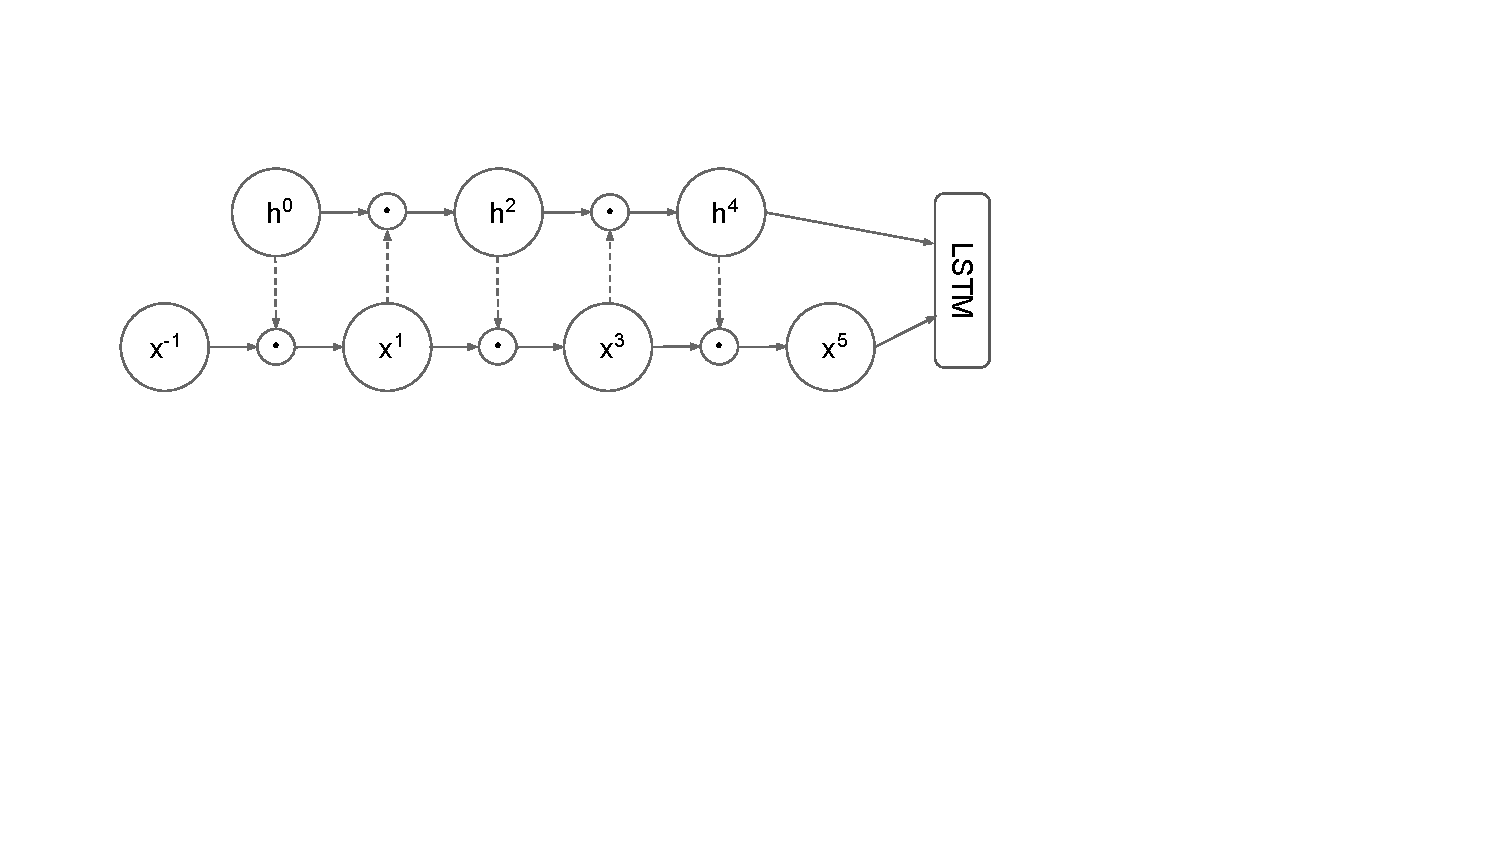
\includegraphics[scale=0.7,trim={1.8cm 7.5cm 8.3cm 2.5cm},clip]
                  {mogrifier/figure/mogrifier.pdf}
  \caption[Mogrifier with 5 rounds of updates.]{Mogrifier with
    5 rounds of updates. The previous state $\vh^0=\vhprev$ is
    transformed linearly (dashed arrows), fed through a sigmoid and
    gates $\vx^{-1}=\vx$ in an elementwise manner producing $\vx^1$.
    Conversely, the linearly transformed $\vx^1$ gates $\vh^0$ and
    produces $\vh^2$. After a number of repetitions of this mutual
    gating cycle, the last values of $\vh^*$ and $\vx^*$ sequences are
    fed to an LSTM cell. The \emph{prev} subscript of $\vh$ is omitted
    to reduce clutter.}
  \label{fig:mogrifier}
\end{figure}
%
While the LSTM is typically presented as a solution to the vanishing
gradients problem, its gate $i$ can also be interpreted as scaling the
rows of weight matrices $\mW^{j*}$ (ignoring the non-linearity in
$j$).
%
In this sense, the LSTM nudges Elman Networks towards
context-dependent transitions and the extreme case of Input Switched
Affine Networks.
%
If we took another, larger step towards that extreme, we could end up
with Hypernetworks \citep{ha2016hypernetworks}.
%
Here, instead, we take a more cautious step and equip the LSTM with
gates that scale the \emph{columns} of all its weight matrices
$\mW^{**}$ in a context-dependent manner.
%
The scaling of the matrices $\mW^{*x}$ (those that transform the cell
input) makes the input embeddings dependent on the cell state, while
the scaling of $\mW^{*h}$ does the reverse.

As \Cref{fig:mogrifier} illustrates, the Mogrifier\footnote{It's like
a transmogrifier\footnotemark{} without the magic: it can only shrink
or expand objects.}\footnotetext{Transmogrify (verb, 1650s): to
completely alter the form of something in a surprising or magical
manner.}
LSTM is an LSTM where two inputs $\vhprev$ and $\vx$ modulate
one another in an alternating fashion before the usual LSTM
computation takes place.
That is,
\begin{gather*}
\mathrm{MogrifierLSTM} \colon \Rb^n\times\Rb^n \times \Rb^m \to \Rb^n \times \Rb^n \\
\LSTM\bigl(\vcprev, \mogrify(\vhprev, \vx)\bigr) = \bigl(\vc, \vh\bigr),
\end{gather*}
where the mogrification operation is the following $\Rb^n\times\Rb^m \to \Rb^n \times \Rb^m$ function:
{\def\groundprop{1.5}
\begin{equation}
\label{eq:mogrify}
\begin{aligned}
  \mogrify(\vh,\vx) &= \vh^{2\floor{r/2}}, \vx^{2\floor{(r+1)/2}-1}\\
  \vx^{-1}, \vh^0 &= \vx, \vh\\
  \vx^i &= 2\sigma\bigl(\mQ^{i}\vh^{i-1}\bigr) \odot \vx^{i-2} &
  \text{for odd i} \in [1..r],\\
  \vh^i &= 2\sigma\bigl(\mR^{i}\vx^{i-1}\bigr) \odot \vh^{i-2}
  & \text{for even i} \in [1..r].
\end{aligned}
\end{equation}}%
Here, the number of rounds, $r \in \Nb$, is a hyperparameter;
$r=0$ recovers the identity function.
%
Multiplication with the constant $2$ ensures that randomly initialized
$\mQ^{i}, \mR^{i}$ matrices result in transformations close to
identity.
%
To reduce the number of additional model parameters, we typically
factorize the $\mQ^{i}, \mR^{i}$ matrices as products of low-rank
matrices: $\mQ^i = \mQ^i_{\textrm{left}} \mQ^i_{\textrm{right}}$ with
$\mQ^i \in \Rb^{m \times n}, \mQ^i_{\textrm{left}} \in
\Rb^{m \times k}, \mQ^i_{\textrm{right}} \in \Rb^{k
  \times n}$, where $k<min(m,n)$ is the rank.\\[-\groundskip]

\section{Experiments}

\subsection{Datasets}

We compare models on both word and character-level language modelling
datasets.
%
The two word-level datasets we picked are the Penn Treebank (\ptb)
corpus by \citet{marcus1993building} with preprocessing from
\citet{mikolov2010recurrent} and \wikitexttwo by
\citet{DBLP:journals/corr/MerityXBS16}, which is about twice the size
of \ptb with a larger vocabulary and lighter preprocessing.
%
These datasets are definitely on the small side, but --~and
\emph{because} of this~-- they are suitable for exploring different
model biases.
%
Their main shortcoming is the small vocabulary size, only in the tens
of thousands, which makes them inappropriate for exploring the
behaviour of the long tail.
%
For that, open vocabulary language modelling and byte pair encoding
\citep{sennrich2015neural} would be an obvious choice.
%
Still, our primary goal here is the comparison of the LSTM and
Mogrifier architectures, thus we instead opt for character-based
language modelling tasks, where vocabulary size is not an issue, the
long tail is not truncated, and there are no additional
hyperparameters as in byte pair encoding that make fair comparison
harder.
%
The first character-based corpus is \enwik from the Hutter Prize
dataset \citep{hutter2012human}.
%
Following common practice, we use the first 90 million characters for
training and the remaining 10 million evenly split between validation
and test.
%
The character-level task on the Mikolov preprocessed \ptb corpus
\citep{merity2018analysis} is unique in that it has the disadvantages
of closed vocabulary without the advantages of word-level modelling,
but we include it for comparison to previous work.
%
The final character-level dataset is the Multilingual Wikipedia Corpus
(MWC, \cite{kawakami2017learning}), from which we focus on the English
and Finnish language subdatasets in the single text, large setting.

\begin{table}[t]
  \caption[Word-level perplexities of near state-of-the-art
    models.]{Word-level perplexities of near state-of-the-art
    models, our LSTM baseline and the Mogrifier on
    \ptb and \wikitexttwo. Models with Mixture of Softmaxes
    \citep{yang2017breaking} are denoted with \emph{MoS}, depth N with
    \emph{dN}. \emph{MC} stands for Monte Carlo dropout evaluation.
    Previous state-of-the-art results in italics. Note the comfortable
    margin of 2.8--4.3 perplexity points the Mogrifier enjoys over the
    LSTM.}
  \label{tab:mog-word-results}
  \small
  \centering
  \begin{tabular}{@{}llrlrlr@{}}
    & & & \multicolumn{2}{c}{No Dyneval} & \multicolumn{2}{c}{Dyneval} \\
    \cmidrule(lr){4-5} \cmidrule(l){6-7}
    & & & Val. & Test & Val. & Test \\
    \midrule
    \parbox[t]{2mm}{\multirow{7}{*}{\rotatebox[origin=c]{90}{PTB}}}
    & FRAGE (d3, MoS15) \citep{gong2018frage} & 22M
        & \emph{54.1} & \emph{52.4} & \emph{47.4} & \emph{46.5} \\
    & AWD-LSTM (d3, MoS15) \citep{yang2017breaking} & 22M
        & 56.5 & 54.4 & 48.3 & 47.7 \\
    & Transformer-XL \citep{dai2019transformer} & 24M
        & 56.7 & 54.5 & & \\
    & \textbf{LSTM} (d2) & 24M
        & \nlltoppl{4.02163} & \nlltoppl{3.99985}
        & \nlltoppl{3.88947} & \nlltoppl{3.88038} \\
    & \textbf{Mogrifier} (d2) & 24M
        & \nlltoppl{3.95346} & \nlltoppl{3.93124}
        & \nlltoppl{3.80963} & \nlltoppl{3.80708} \\
    & \textbf{LSTM} (d2, MC) & 24M
        & \nlltoppl{4.01559} & \nlltoppl{3.99003}
        & \nlltoppl{3.88338} & \nlltoppl{3.87987} \\
    & \textbf{Mogrifier} (d2, MC) & 24M
        & \nlltopplbold{3.93959} & \nlltopplbold{3.91415}
        & \nlltopplbold{3.80420} & \nlltopplbold{3.80321} \\
    \midrule
    \parbox[t]{2mm}{\multirow{6}{*}{\rotatebox[origin=c]{90}{WT$2$}}}
    & FRAGE (d3, MoS15) \citep{gong2018frage} & 35M
        & \emph{60.3} & \emph{58.0} & \emph{40.8} & \emph{39.1} \\
    & AWD-LSTM (d3, MoS15) \citep{yang2017breaking} & 35M
        & 63.9 & 61.2 & 42.4 & 40.7 \\
    & \textbf{LSTM} (d2, MoS2) & 35M
        & \nlltoppl{4.13609} & \nlltoppl{4.09557}
        & \nlltoppl{3.76661} & \nlltoppl{3.72658} \\
    & \textbf{Mogrifier} (d2, MoS2) & 35M
        & \nlltoppl{4.07235} & \nlltoppl{4.03665}
        & \nlltoppl{3.70429} & \nlltoppl{3.66475} \\
    & \textbf{LSTM} (d2, MoS2, MC) & 35M
        & \nlltoppl{4.12526} & \nlltoppl{4.08426}
        & \nlltoppl{3.76540} & \nlltoppl{3.72385} \\
    & \textbf{Mogrifier} (d2, MoS2, MC) & 35M
        & \nlltopplbold{4.04771} & \nlltopplbold{4.00976}
        & \nlltopplbold{3.69399} & \nlltopplbold{3.65337} \\
    \midrule
  \end{tabular}
\end{table}

\subsection{Setup}

We tune hyperparameters following the experimental setup of
\cite{melis2018pushing} using a black-box hyperparameter tuner based
on batched Gaussian Process Bandits \citep{golovin2017google}.
%
For the LSTM, the tuned hyperparameters are the same:
\emph{input\_embedding\_ratio}, \emph{learning\_rate},
\emph{l2\_penalty}, \emph{input\_dropout},
\emph{inter\_layer\_dropout}, \emph{state\_dropout},
\emph{output\_dropout}.
%
For the Mogrifier, the number of rounds $r$ and the rank $k$ of the
low-rank approximation is also tuned (allowing for full rank, too).
%
For word-level tasks, BPTT \citep{werbos1990backpropagation} window
size is set to 70 and batch size to 64.
%
For character-level tasks, BPTT window size is set to 150 and batch
size to 128 except for \enwik where the window size is 500.
%
Input and output embeddings are tied for word-level tasks following
\cite{DBLP:journals/corr/InanKS16} and
\cite{DBLP:journals/corr/PressW16}.
%
Optimization is performed with Adam \citep{kingma2014adam} with
$\beta_1=0$, a setting that resembles RMSProp without momentum.
%
Gradients are clipped \citep{pascanu2013difficulty} to norm 10.
%
We switch to averaging weights similarly to
\cite{merity2017regularizing} after a certain number of checkpoints
with no improvement in validation cross-entropy or at 80\% of the
training time at the latest.
%
We found no benefit to using two-step finetuning.

Model evaluation is performed with the standard, deterministic dropout
approximation or Monte Carlo averaging \citep{gal2016theoretically}
where explicitly noted (MC).
%
In standard dropout evaluation, dropout is turned off while in MC
dropout predictions are averaged over randomly sampled dropout masks
(200 in our experiments).
%
Optimal softmax temperature is determined on the validation set, and
in the MC case, dropout rates are scaled \citep{melis2018pushing}.
%
Finally, we report results with and without dynamic evaluation
\citep{krause2017dynamic}.
%
Hyperparameters for dynamic evaluation are tuned using the same method
(see \Cref{sec:hyperparameter-tuning-ranges} for details).

%% We make the code and the tuner output available at
%% \href{https://github.com/deepmind/lamb}{https://github.com/deepmind/lamb}.

\begin{table}[t!]
  \caption[Bits per character on character-based datasets of near
    state-of-the-art models.]{Bits per character on
    character-based datasets of near state-of-the-art models, our
    LSTM baseline and the Mogrifier. Previous
    state-of-the-art results in italics. Depth N is denoted with
    \emph{dN}. MC stands for Monte Carlo dropout evaluation. Once
    again the Mogrifier strictly dominates the LSTM and sets a new
    state of the art on all but the \enwik dataset where with dynamic
    evaluation it closes the gap to the Transformer-XL of similar size
    ($\dag$ \cite{krause2019dynamic}, $\ddag$ Ben Krause, personal
    communications, May 17, 2019). On most datasets, model size was
    set large enough for underfitting not to be an issue. This was
    very much not the case with \enwik, so we grouped models of
    similar sizes together for ease of comparison. Unfortunately, a
    couple of dynamic evaluation test runs diverged (NaN) on the test
    set and some were just too expensive to run (\enwik, MC).}
  \label{tab:mog-character-results}
  \centering
  \small
  \begin{tabular}{@{}llrllll@{}}
    & & & \multicolumn{2}{c}{No Dyneval} & \multicolumn{2}{c}{Dyneval} \\
    \cmidrule(lr){4-5} \cmidrule(lr){6-7}
    & & & Val. & \multicolumn{1}{r}{Test} & Val. & \multicolumn{1}{r}{Test} \\
    \midrule
    \parbox[t]{2mm}{\multirow{6}{*}{\rotatebox[origin=c]{90}{PTB}}}
    & Trellis Networks \citep{bai2018trellis} & 13.8M & & \emph{1.159} & & \\
    & AWD-LSTM (d3) \citep{merity2017regularizing} & 13.8M & & 1.175 & & \\
    & \textbf{LSTM} (d2) & 24M
        & \nlltobpc{0.80641} & \nlltobpc{0.79259}
        & \nlltobpc{0.77349} & \nlltobpc{0.76448} \\
    & \textbf{Mogrifier} (d2) & 24M
        & \nlltobpc{0.79616} & \nlltobpc{0.78415}
        & \nlltobpc{0.76119} & \nlltobpc{0.75439} \\
    & \textbf{LSTM} (d2, MC) & 24M
        & \nlltobpc{0.80331} & \nlltobpc{0.78936}
        & \nlltobpc{0.77262} & \nlltobpc{0.76353} \\
    & \textbf{Mogrifier} (d2, MC) & 24M
        & \nlltobpcbold{0.78829} & \nlltobpcbold{0.77642}
        & \nlltobpcbold{0.75861} & \nlltobpcbold{0.75069} \\
    \midrule
    \multirow{6}{*}{\rotatebox[origin=c]{90}{MWC\,\, EN}}
    & HCLM+Cache \citep{kawakami2017learning} & 8M
        & \emph{1.591} & \emph{1.538} & & \\
    & LSTM (d1) \citep{kawakami2017learning} & 8M
        & 1.793 & 1.736 & & \\
    & \textbf{LSTM} (d2) & 24M
        & \nlltobpc{0.93766} & \nlltobpc{0.92752}
        & \nlltobpc{0.85915} & \nlltobpc{0.84918} \\
    & \textbf{Mogrifier} (d2) & 24M
        & \nlltobpc{0.91464} & \nlltobpc{0.90439}
        & \nlltobpc{0.83346} & \nlltobpc{0.82386} \\
    & \textbf{LSTM} (d2, MC) & 24M
        & \nlltobpc{0.93336} & \nlltobpc{0.92356}
        & \nlltobpc{0.85783} & NaN \\
    & \textbf{Mogrifier} (d2, MC) & 24M
        & \nlltobpcbold{0.90977} & \nlltobpcbold{0.89980}
        & \nlltobpcbold{0.83193} & \nlltobpcbold{0.82302} \\
    \midrule
    \multirow{6}{*}{\rotatebox[origin=c]{90}{MWC\,\, FI}}
    & HCLM+Cache \citep{kawakami2017learning} & 8M
        & \emph{1.754} & \emph{1.711} & & \\
    & LSTM (d1) \citep{kawakami2017learning} & 8M
        & 1.943 & 1.913 & & \\
    & \textbf{LSTM} (d2) & 24M
        & \nlltobpc{0.95833} & \nlltobpc{0.94772}
        & \nlltobpc{0.86577} & \nlltobpc{0.85727} \\
    & \textbf{Mogrifier} (d2) & 24M
        & \nlltobpc{0.92782} & \nlltobpc{0.91896}
        & \nlltobpc{0.83318} & \nlltobpcbold{0.82591} \\
    & \textbf{LSTM} (d2, MC) & 24M
        & \nlltobpc{0.95456} & \nlltobpc{0.94337}
        & \nlltobpc{0.86415} & \nlltobpc{0.85556} \\
    & \textbf{Mogrifier} (d2, MC) & 24M
        & \nlltobpcbold{0.91995} & \nlltobpcbold{0.91050}
        & \nlltobpcbold{0.83029} & NaN \\
    \midrule
    \parbox[t]{2mm}{\multirow{13}{*}{\rotatebox[origin=c]{90}{\enwik}}}
    & Transformer-XL (d24) \citep{dai2019transformer} & 277M
        & & \textbf{0.993} & & \textbf{0.940}$\dag$ \\
    \cmidrule(l){2-7}
    & Transformer-XL (d18) \citep{dai2019transformer} & 88M
        & & 1.03 & & \\
    & \textbf{LSTM} (d4) & 96M
        & \nlltobpc{0.79343} & \nlltobpc{0.80062}
        & \nlltobpc{0.72191} & \nlltobpc{0.70699} \\
    & \textbf{Mogrifier} (d4) & 96M
        & \nlltobpc{0.76935} & \nlltobpc{0.77792}
        & \nlltobpc{0.69911} & \nlltobpc{0.68516} \\
    & \textbf{LSTM} (d4, MC) & 96M
        & \nlltobpc{0.78948} & \nlltobpc{0.79511}
        & & \\
    & \textbf{Mogrifier} (d4, MC) & 96M
        & \nlltobpc{0.76566} & \nlltobpc{0.77359}
        & & \\
    \cmidrule(l){2-7}
    & Transformer-XL (d12) \citep{dai2019transformer} & 41M
        & & 1.06 & & 1.01$\ddag$ \\
    & AWD-LSTM (d3) \citep{merity2017regularizing} & 47M
        & & 1.232 & & \\
    & mLSTM (d1) \citep{DBLP:journals/corr/KrauseLMR16} & 46M
        & & 1.24 & & 1.08 \\
    & \textbf{LSTM} (d4) & 48M
        & \nlltobpc{0.81915} & \nlltobpc{0.82841}
        & \nlltobpc{0.74416} & \nlltobpc{0.72877} \\
    & \textbf{Mogrifier} (d4) & 48M
        & \nlltobpc{0.78663} & \nlltobpc{0.79413}
        & \nlltobpc{0.71751} & \nlltobpc{0.70177} \\
    & \textbf{LSTM} (d4, MC) & 48M
        & \nlltobpc{0.81555} & \nlltobpc{0.82346}
        & & \\
    & \textbf{Mogrifier} (d4, MC) & 48M
        & \nlltobpc{0.78368} & \nlltobpc{0.79054}
        & & \\
    \midrule
  \end{tabular}
\end{table}

\subsection{Results}
\label{sec:results}

\Cref{tab:mog-word-results} lists our results on word-level
datasets.
%
On the \ptb and \wikitexttwo datasets, the Mogrifier has lower
perplexity than the LSTM by 3--4 perplexity points regardless of
whether or not dynamic evaluation \citep{krause2017dynamic} and
Monte Carlo averaging are used.
%
On both datasets, the state of the art is held by the AWD LSTM
\citep{merity2017regularizing} extended with Mixture of Softmaxes
\citep{yang2017breaking} and FRAGE \citep{gong2018frage}.
%
The Mogrifier improves the state of the art without either of these
methods on \ptb, and without FRAGE on \wikitexttwo.

\Cref{tab:mog-character-results} lists the character-level modelling
results.
%
On all datasets, our baseline LSTM results are much better than those
previously reported for LSTMs, highlighting the issue of scalability
and experimental controls.
%
In some cases, these unexpectedly large gaps may be down to lack of
hyperparameter tuning as in the case of \cite{merity2017regularizing},
or in others, to using a BPTT window size (50) that is too small for
character-level modelling \citep{melis2017state} in order to fit the
model into memory.
%
The Mogrifier further improves on these baselines by a considerable
margin.
%
Even the smallest improvement of 0.012 bpc on the highly
idiosyncratic, character-based, Mikolov preprocessed \ptb task is
equivalent to gaining about 3 perplexity points on word-level \ptb.
%
MWC, which was built for open-vocabulary language modelling, is a much
better smaller-scale character-level dataset.
%
On the English and the Finnish corpora in MWC, the Mogrifier enjoys a
gap of 0.033--0.046 bpc.
%
Finally, on the \enwik dataset, the gap is 0.029--0.039 bpc in favour
of the Mogrifier.

Of particular note is the comparison to Transformer-XL
\citep{dai2019transformer}, a state-of-the-art model on larger
datasets such as Wikitext-103 and \enwik.
%
On \ptb, without dynamic evaluation, the Transformer-XL is on par with
our LSTM baseline which puts it about 3.5 perplexity points behind the
Mogrifier.
%
On \enwik, also without dynamic evaluation, the Transformer-XL has a
large, 0.09 bpc advantage at similar parameter budgets, but with
dynamic evaluation this gap disappears.
%
However, we did not test the Transformer-XL ourselves, so fair
comparison is not possible due to differing experimental setups and
the rather sparse result matrix for the Transformer-XL.

\section{Analysis}
\label{sec:mog-analysis}

\subsection{Ablation Study}

The Mogrifier consistently outperformed the LSTM in our experiments.
%
The optimal settings were similar across all datasets, with $r \in
\{5,6\}$ and $k \in [40..90]$ (see
\Cref{sec:hyperparameter-sensitivity} for a discussion of
hyperparameter sensitivity).
%
In this section, we explore the effect of these hyperparameters and
show that the proposed model is not unnecessarily complicated.
%
To save computation, we tune all models using a shortened schedule
with only 145 epochs instead of 964 and a truncated BPTT window size
of 35 on the word-level PTB dataset, and evaluate using the standard,
deterministic dropout approximation with a tuned softmax temperature.

\Cref{fig:ppl-vs-rounds} shows that the number of rounds $r$
greatly influences the results.
%
Second, we found the low-rank factorization of $\mQ^i$ and $\mR^i$ to
help a bit, but the full-rank variant is close behind, which is what we
observed on other datasets, as well.
%
Finally, to verify that the alternating gating scheme is not overly
complicated, we condition \emph{all} newly introduced gates on the
original inputs $\vx$ and $\vhprev$ (see \Cref{fig:mogrifier-no-zigzag}).
%
\begin{figure}[!t]\centering
  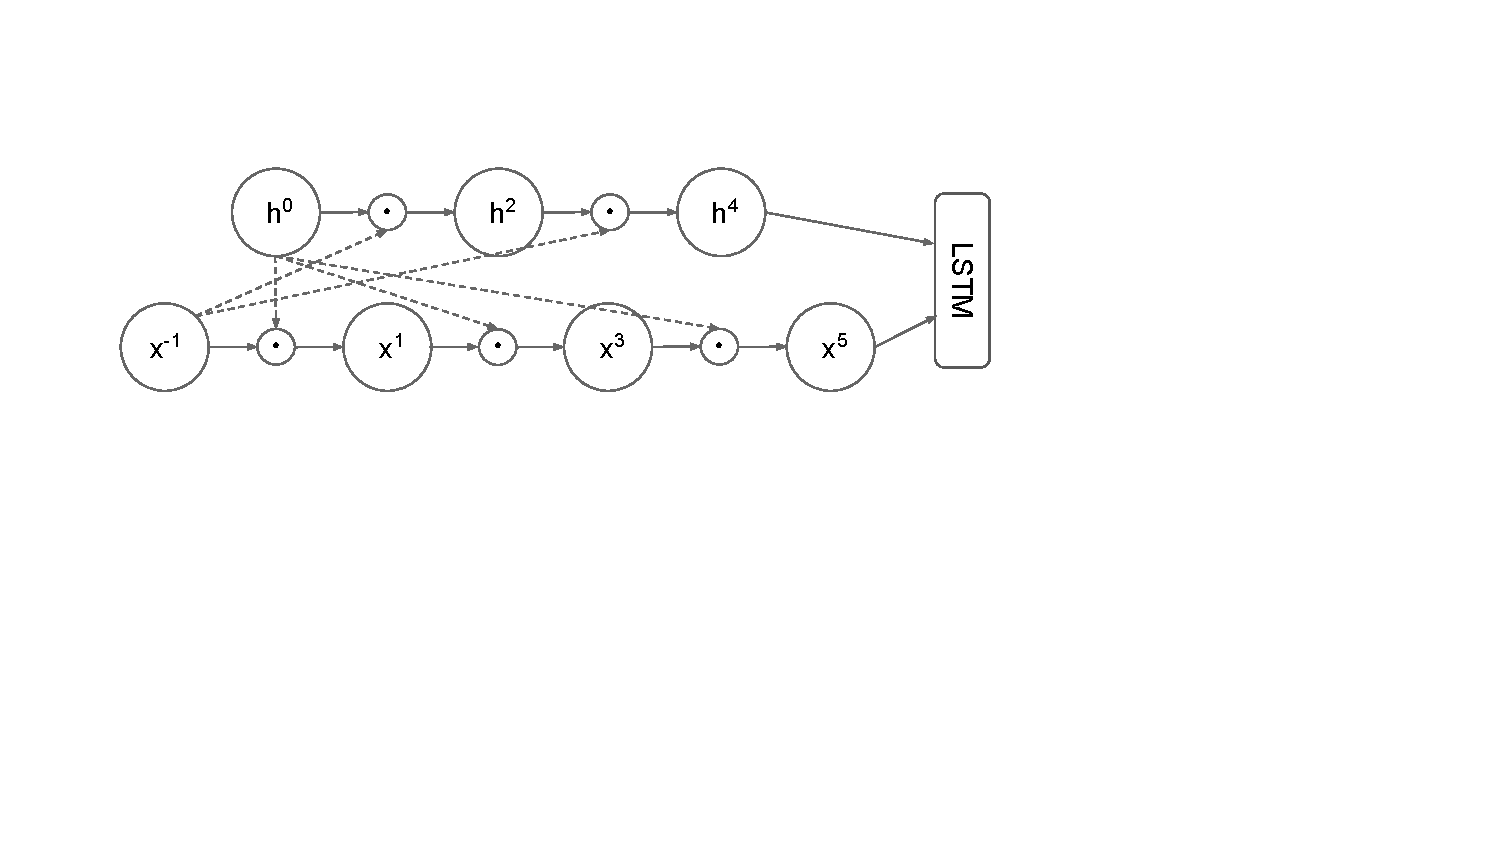
\includegraphics[scale=0.7,trim={1.8cm 7.5cm 8.3cm 2.5cm},clip]
                  {mogrifier/figure/mogrifier-no-zigzag.pdf}
  \caption[No-zigzag Mogrifier for the ablation study.]{No-zigzag Mogrifier for the ablation study, whose gating is always based on the original inputs.}
  \label{fig:mogrifier-no-zigzag}
\end{figure}
%
That is, in \eqref{eq:mogrify} the updates are changed to these no-zigzag variants:
\begin{align*}
  \vx^i &= 2\sigma\bigl(\mQ^{i}\vhprev\bigr) \odot \vx^{i-2} &
  \text{for odd i} \in [1..r],\\
  \vhprev^i &= 2\sigma\bigl(\mR^{i}\vx\bigr) \odot \vhprev^{i-2}
  & \text{for even i} \in [1..r].
\end{align*}
In our experiments, the no-zigzag variant underperformed the baseline
Mogrifier by a small but significant margin, and was on par with the
$r=2$ model in \Cref{fig:ppl-vs-rounds} suggesting that the
Mogrifier's iterative refinement scheme does more than simply widen
the range of possible gating values of $\vx$ and $\vhprev$ to $(0,
2^{\lceil r/2 \rceil})$ and $(0, 2^{\lfloor r/2 \rfloor})$,
respectively.

\begin{figure}
\begin{minipage}{0.5\linewidth}
  \begin{tikzpicture}
    \begin{axis}[width=1.05\linewidth, height=3.8cm,
        x label style={at={(axis description cs:0.5,-0.15)},anchor=north},
        y label style={at={(axis description cs:-0.11,.5)},rotate=0,
                       anchor=south},
        xlabel=$r$ rounds,
        ylabel=PPL,
        cycle list name=acycle]
	\addplot+ coordinates {
	  (0, 57.5) (1, 56.4) (2, 55.5)
          (3, 54.82) (4, 54.1) (5, 54.3) (6, 54.6)
	};
    \end{axis}
  \end{tikzpicture}
\captionof{figure}{Perplexity vs the number of rounds $r$ in the \ptb ablation
  study.}
\label{fig:ppl-vs-rounds}
\end{minipage}
\hfill
\begin{minipage}{0.46\linewidth}
\setlength\tabcolsep{36pt}
\begin{tabularx}{\textwidth}{@{}lr@{}}
  \midrule
  Mogrifier      & \nlltoppl{3.99163}  \\
  Full rank $Q^i,P^i$ & \nlltoppl{3.99947} \\
  No zigzag      & \nlltoppl{4.00647} \\
  LSTM           & \nlltoppl{4.051} \\
  mLSTM          & \nlltoppl{4.05750} \\
  \midrule
\end{tabularx}
\vspace{0.6\baselineskip}
\captionof{table}{PTB ablation study
  validation perplexities with 24M parameters.}
\label{tab:ablation}
\end{minipage}
\end{figure}

\subsection{Comparison to the mLSTM}
\label{seq:comparison-to-the-mlstm}

The Multiplicative LSTM \citep{DBLP:journals/corr/KrauseLMR16}, or
mLSTM for short, is closest to our model in the literature.
%
Formulating it as
\begin{gather*}
\mLSTM\bigl(\vx, \vcprev, \vhprev\bigr) = \LSTM\bigl(\vx, \vcprev, \vhprev^m\bigr)\\
\vhprev^m = \bigl(\mW^{mx} \vx\bigr) \odot \bigl(\mW^{mh} \vhprev\bigr),
\end{gather*}
%
the differences are readily apparent.
%
First, the mLSTM allows for multiplicative interaction between $\vx$
and $\vhprev$, but it only overrides $\vhprev$, while in the Mogrifier
the interaction is two-way, which --~as the ablation study showed~--
is important.
%
Second, the mLSTM can change not only the magnitude but also the sign
of values in $\vhprev$, something with which we experimented in the
Mogrifier, but could not get to work.
%
Furthermore, in the definition of $\vhprev^m$, the unsquashed
linearities and their elementwise product make the mLSTM more
sensitive to initialization and unstable during optimization.

On the \enwik dataset, we greatly improved on the published results of
the mLSTM \citep{DBLP:journals/corr/KrauseLMR16}.
%
In fact, even our LSTM baseline outperformed the mLSTM by 0.03 bpc.
%
We also conducted experiments on \ptb based on our reimplementation of
the mLSTM following the same methodology as the ablation study and
found that the mLSTM did not improve on the LSTM (see
\Cref{tab:ablation}).

\cite{DBLP:journals/corr/KrauseLMR16} posit and verify the recovery
hypothesis that says that having just suffered a large loss, the loss
on the next time step will be smaller on average for the mLSTM than
for the LSTM.
%
This was found not to be the case for the Mogrifier.
%
Neither did we observe a significant change in the gap between the
LSTM and the Mogrifier in the tied and untied embeddings settings,
which would be expected if recovery was affected by $\vx$ and
$\vhprev$ being in different domains.

\subsection{The Reverse Copy Task}

Our original motivation for the Mogrifier was to allow the context to
amplify salient and attenuate nuisance features in the input
embeddings.
%
We conduct a simple experiment to support this point of view.
%
Consider the reverse copy task where the network reads an input
sequence of tokens and a marker token after which it has to repeat the
input in reverse order.
%
In this simple sequence-to-sequence learning
\citep{sutskever2014sequence} setup, the reversal is intended to avoid
the minimal time lag problem \citep{hochreiter1997lstm}, which is not
our focus here.

The experimental setup is as follows.
%
For the training set, we generate \num{500000} examples by uniformly
sampling a given number of tokens from a vocabulary of size
\num{1000}.
%
The validation and test sets are constructed similarly, and contain
\num{10000} examples.
%
The model consists of an independent, unidirectional encoder and a
decoder, whose total number of parameters is \num{10} million.
%
The decoder is initialized from the last state of the encoder.
%
Since overfitting is not an issue here, no dropout is necessary, and
we only tune the learning rate, the l2 penalty, and the embedding size for
the LSTM.
%
For the Mogrifier, the number of rounds $r$ and the rank $k$ of the
low-rank approximation are also tuned.

\begin{figure}[!t]
  \begin{subfigure}{0.49\linewidth}
  \begin{tikzpicture}
    \begin{axis}[width=1.1 \linewidth, height=4.5cm,
        legend pos = north west,
        legend style={font=\footnotesize},
        x label style={at={(axis description cs:0.5,-0.15)},anchor=north},
        y label style={at={(axis description cs:-0.1,.5)},rotate=0,
                       anchor=south},
        xlabel=sequence length,
        ylabel=XE,
        cycle list name=acycle]
	\addplot+ coordinates {
		(50, 0.00020) (100, 0.05715) (150, 0.62399) (200, 1.80348)
	};
	\addplot+ coordinates {
		(50, 0.00038) (100, 0.07821) (150, 0.27998) (200, 1.39342)
	};
    \legend{$LSTM$,$Mogrifier$}
    \end{axis}
  \end{tikzpicture}
  \caption{10M parameters with vocabulary size 1k.}
  \label{fig:copy-10m-results}
  \end{subfigure}
  \hfill
  \begin{subfigure}{0.47\linewidth}
  \begin{tikzpicture}
    \begin{axis}[width=1.1\linewidth, height=4.5cm,
        legend pos = north west,
        legend style={font=\footnotesize},
        x label style={at={(axis description cs:0.5,-0.15)},anchor=north},
        y label style={at={(axis description cs:-0.1,.5)},rotate=0,
                       anchor=south},
        xlabel=sequence length,
        ylabel=XE,
        cycle list name=acycle]
	\addplot+ coordinates {
		(50, 0.14) (100, 0.25) (150, 1.49) (200, 3.99)
	};
	\addplot+ coordinates {
		(50, 0.03) (100, 0.13) (150, 0.29) (200, 1.03)
	};
    \legend{$LSTM$,$Mogrifier$}
    \end{axis}
  \end{tikzpicture}
  \caption{24M parameters with vocabulary size 10k.}
  \label{fig:copy-24m-results}
  \end{subfigure}
  \caption[Cross-entropy vs sequence length in the reverse copy
    task.]{Cross-entropy vs sequence length in the reverse copy
    task with i.i.d.\ tokens. Lower is better. The Mogrifier is better
    than the LSTM even in this synthetic task with no resemblance to
    natural language.}
\end{figure}

We compare the case where both the encoder and decoder are LSTMs to
where both are Mogrifiers.
%
\Cref{fig:copy-10m-results} shows that, for sequences of length
50 and 100, both models can solve the task perfectly.
%
At higher lengths though, the Mogrifier has a considerable advantage.
%
Examining the best hyperparameter settings found, the embedding/hidden
sizes for the LSTM and Mogrifier are 498/787 vs 41/1054 at 150 steps,
and 493/790 vs 181/961 at 200 steps.
%
Clearly, the Mogrifier was able to work with a much smaller embedding
size than the LSTM, which is in line with our expectations for a model
with a more flexible interaction between the input and recurrent
state.
%
We also conducted experiments with a larger model and vocabulary size,
and found the effect even more pronounced (see
\Cref{fig:copy-24m-results}).

\subsection{What the Mogrifier is Not}

The results on the reverse copy task support our hypothesis that input
embeddings are enriched by the Mogrifier architecture, but that cannot
be the full explanation as the results of the ablation study indicate.
%
In the following, we consider a number of hypotheses about where the
advantage of the Mogrifier lies and the experiments that provide
evidence \emph{against} them.
\begin{itemize}
\renewcommand\labelitemi{\scriptsize\Lightning}
\item \emph{Hypothesis: the benefit is in scaling $\vx$ and
  $\vhprev$.} We verified that data dependency is a crucial feature by
  adding a learnable scaling factor to the LSTM inputs. We observed no
  improvement. Also, at extremely low-rank (less than 5) settings
  where the amount of information in its gating is small, the
  Mogrifier loses its advantage.
\item \emph{Hypothesis: the benefit is in making optimization easier.}
  We performed experiments with different optimizers (SGD, RMSProp),
  with intra-layer batch normalization and layer normalization on the
  LSTM gates. While we cannot rule out an effect on optimization
  difficulty, in all of these experiments the gap between the LSTM and
  the Mogrifier was the same.
\item \emph{Hypothesis: exact tying of embeddings is too constraining,
  the benefit is in making this relationship less strict.} Experiments
  conducted with untied embeddings and character-based models
  demonstrate improvements of similar magnitude.
\item \emph{Hypothesis: the benefit is in the low-rank factorization
  of $\mQ^{i}, \mR^{i}$ implicitly imposing structure on the LSTM
  weight matrices.} We observed that the full-rank Mogrifier also
  performed better than the plain LSTM. We conducted additional
  experiments where the LSTM's gate matrices were factorized and
  observed no improvement.
\item \emph{Hypothesis: the benefit comes from better performance on
  rare words.} The observed advantage on character-based modelling is
  harder to explain based on frequency. Also, in the reverse copy
  experiments, a large number of tokens were sampled uniformly, so
  there were no rare words to speak of.
\item \emph{Hypothesis: the benefit is specific to the English
  language.} The improvements observed on the Finnish dataset and the
  reverse copy experiments, which did not feature natural language at
  all, directly contradict this hypothesis.
\item \emph{Hypothesis: the benefit is in handling long-range
  dependencies better.} Experiments in the episodic setting (i.e.
  sentence-level language modelling) exhibited the same gap as the
  non-episodic ones.
\item \emph{Hypothesis: the scaling up of inputs saturates the
  downstream LSTM gates.} The idea here is that saturated gates may
  make states more stable over time. We observed the opposite: the
  means of the standard LSTM gates in the Mogrifier were very close
  between the two models, but their variance was smaller in the
  Mogrifier.
\end{itemize}

\section{Conclusions}

\mglconclusion
Many advances in natural language processing have been based upon more
expressive models for how inputs interact with the context in which
they occur.
%
Recurrent networks, which have enjoyed a modicum of success, still
lack the generalization and systematicity ultimately required for
modelling language.
%
In this work, we proposed an extension to the venerable Long Short-Term
Memory in the form of mutual gating of the current input and the
previous output.
%
This mechanism affords the modelling of a richer space of interactions
between inputs and their context.
%
Equivalently, our model can be viewed as making the transition
function given by the LSTM context-dependent.
%
Experiments demonstrate markedly improved generalization on language
modelling in the range of 3--4 perplexity points on Penn Treebank and
\wikitexttwo, and 0.01--0.05 bpc on four character-based datasets.
%
With the Mogrifier LSTM, we establish a new state of the art on all
datasets with the exception of \enwik, where we close a large gap
between the LSTM and Transformer models.

Our original motivation for this work was that the context-free
representation of input tokens may be a bottleneck in language models,
and by conditioning the input embedding on the recurrent state some
benefit was indeed derived.
%
While it may be part of the explanation, this interpretation clearly
does not account for the improvements brought by conditioning the
recurrent state on the input and especially the benefits of mogrification on
character-level datasets.
%
Positioning our work on the Multiplicative RNN line of research offers
a more compelling perspective.

To give more credence to this interpretation, in the analysis we
highlighted a number of possible alternative explanations and ruled
them all out to varying degrees.
%
In particular, the connection to the mLSTM was found to be weaker than
expected as the Mogrifier does not exhibit improved recovery (see
\Cref{seq:comparison-to-the-mlstm}), and on \ptb the mLSTM
works only as well as the LSTM.
%
At the same time, the evidence against easier optimization is weak,
and the Mogrifier establishing some kind of sharing between otherwise
independent LSTM weight matrices is a distinct possibility.

Finally, note that as shown by \Cref{fig:mogrifier} and
\eqref{eq:mogrify}, the Mogrifier is a series of preprocessing
steps composed with the LSTM function, but other architectures, such
as Mogrifier GRU or Mogrifier Elman Network are possible.
%
We also leave investigations into other forms of parameterization of
context-dependent transitions for future work.

\mglsep

\chapter*{Appendices}

\begin{subappendices}

\section{Hyperparameter Tuning Ranges}
\label{sec:hyperparameter-tuning-ranges}

In all experiments, we tuned hyperparameters using Google Vizier
\citep{golovin2017google}.
%
The tuning ranges are listed in
\Cref{tab:hyperparameter-tuning-ranges}.
%
Obviously, \emph{mogrifier\_rounds} and \emph{mogrifier\_rank} are
tuned only for the Mogrifier.
%
If $input\_embedding\_ratio \geqslant 1$, then the input/output
embedding sizes and the hidden sizes are set to equal and the linear
projection from the cell output into the output embeddings space is
omitted.
%
Similarly, $mogrifier\_rank \leqslant 0$ is taken to mean full rank
$\mQ^{*}$, $\mR^{*}$ without factorization.
%
Since \enwik is a much larger dataset, we do not tune
\emph{input\_embedding\_ratio} and specify tighter tuning ranges for
dropout based on preliminary experiments (see
\Cref{tab:hyperparameter-tuning-ranges-enwik}).

Dynamic evaluation hyperparameters were tuned according to
\Cref{tab:hyperparameter-tuning-ranges-dyneval}.
%
The highest possible value for \emph{max\_time\_steps}, the BPTT
window size, was 20 for word, and 50 for character-level tasks.
%
The batch size for estimating the mean squared gradients over the
training data was set to 1024, gradient clipping was turned off, and
the l2 penalty was set to zero.

\begin{table}[tp]
  \caption{Hyperparameter tuning ranges for all tasks except
    \enwik.}
  \label{tab:hyperparameter-tuning-ranges}

  \centering
  \begin{tabular}{@{}lrrrr@{}}
    & Low & High & Spacing \\
    \midrule
    learning\_rate & 0.001 & 0.004 & log \\
    input\_embedding\_ratio & 0.0 & 2.0 & \\
    l2\_penalty & 5e-6 & 1e-3 & log \\
    input\_dropout & 0.0 & 0.9 & \\
    inter\_layer\_dropout & 0.0 & 0.95 & \\
    state\_dropout & 0.0 & 0.8 \\
    output\_dropout & 0.0 & 0.95 \\
    mogrifier\_rounds ($r$) & 0 & 6 \\
    mogrifier\_rank ($k$) & -20 & 100 \\
    \midrule
  \end{tabular}
\end{table}

\begin{table}[tp]
  \caption{Hyperparameter tuning ranges for \enwik.}
  \label{tab:hyperparameter-tuning-ranges-enwik}

  \centering
  \begin{tabular}{@{}lrrrr@{}}
    & Low & High & Spacing \\
    \midrule
    learning\_rate & 0.001 & 0.004 & log \\
    l2\_penalty & 5e-6 & 1e-3 & log \\
    input\_dropout & 0.0 & 0.2 & \\
    inter\_layer\_dropout & 0.0 & 0.2 & \\
    state\_dropout & 0.0 & 0.25 \\
    output\_dropout & 0.0 & 0.25 \\
    mogrifier\_rounds ($r$) & 0 & 6 \\
    mogrifier\_rank ($k$) & -20 & 100 \\
    \midrule
  \end{tabular}
\end{table}

\begin{table}[tp]
  \caption{Hyperparameter tuning ranges for dynamic evaluation.}
  \label{tab:hyperparameter-tuning-ranges-dyneval}

  \centering
  \begin{tabular}{@{}lrrrr@{}}
    & Low & High & Spacing \\
    \midrule
    max\_time\_steps & 1 & 20/50 & \\
    dyneval\_learning\_rate & 1e-6 & 1e-3 & log \\
    dyneval\_decay\_rate & 1e-6 & 1e-2 & log \\
    dyneval\_epsilon & 1e-8 & 1e-2 & log \\
    \midrule
  \end{tabular}
\end{table}

\section{Hyperparameter Sensitivity}
\label{sec:hyperparameter-sensitivity}

The parallel coordinate plots in \Cref{fig:lstm-sensitivity} and
\ref{fig:fm-sensitivity} give a rough idea about hyperparameter
sensitivity.
%
The red lines correspond to hyperparameter combinations closest to the
best solution found.
%
To find the closest combinations, we restricted the range for each
hyperparameter separately to about 15\% of its entire tuning range.
%
For both the LSTM and the Mogrifier, the results are at most 1.2
perplexity points off the best result, so our results are somewhat
insensitive to jitter in the hyperparameters.
%
Still, in this setup, grid search would require orders of magnitude
more trials to find comparable solutions.

On the other hand, the tuner does take advantage of the stochasticity
of training, and repeated runs with the same parameters may give
slightly worse results.
%
To gauge the extent of this effect, on \ptb we estimated the standard
deviation in reruns of the LSTM with the best hyperparameters to be
about 0.2 perplexity points, but the mean was about 0.7 perplexity
points off the result produced with the weights saved in best tuning
run.

\begin{figure}[tp]\centering
  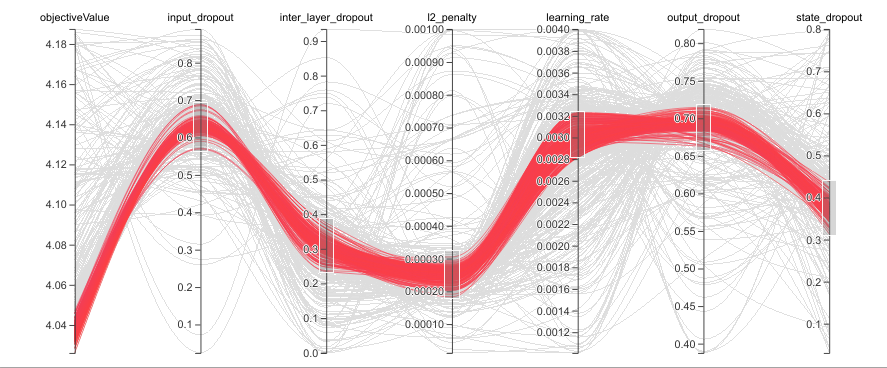
\includegraphics[width=0.98\textwidth,trim={0cm 0.1cm 0.0cm 0cm},clip]
                  {mogrifier/figure/ptb-24m-lstm-d2-sensitivity.png}
  \caption[LSTM hyperparameter sensitivity on PTB.]{Average
    per-word validation cross-entropies for hyperparameter
    combinations in the neighbourhood of the best solution for a
    2-layer LSTM with 24M weights on the Penn Treebank dataset.}
  \label{fig:lstm-sensitivity}
\end{figure}

\begin{figure}[tp]\centering
  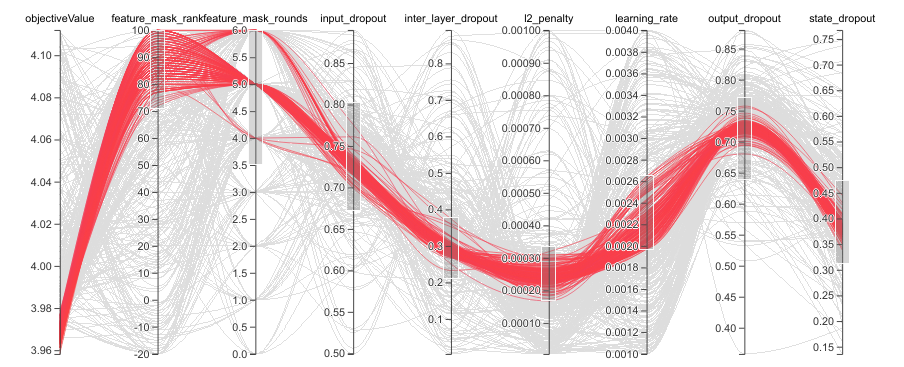
\includegraphics[width=0.98\textwidth,trim={0cm 0.1cm 0.0cm 0cm},clip]
                  {mogrifier/figure/ptb-24m-fm-d2-sensitivity.png}
  \caption[Mogrifier hyperparameter sensitivity on PTB.]{Average
    per-word validation cross-entropies for hyperparameter
    combinations in the neighbourhood of the best solution for a
    2-layer Mogrifier LSTM with 24M weights on the Penn Treebank
    dataset. \emph{feature\_mask\_rank} and
    \emph{feature\_mask\_rounds} are aliases for
    \emph{mogrifier\_rank} and \emph{mogrifier\_rounds}}.
  \label{fig:fm-sensitivity}
\end{figure}

\end{subappendices}



\chapter{Optimization Oomph}
\label{sec:optimization-oomph}

\mglepigraph{0.3}{It's not much of a tail, but I'm sort of attached to it.}{A.A. Milne}
\mgllettrine{findent=-0.2em,nindent=0.4em}{M}{ogrification}
proved surprisingly powerful, but it comes with a performance penalty.
With thorough hyperparemeter tuning (a prerequisite of reliable model evaluation), this penalty and the already high base cost of the LSTM must be paid hundreds of times.
Scaling to larger datasets makes this process even more resource intensive.

More generally, when training a single model is expensive, there are fewer resources left for exploring the design and hyperparameter space, which compromises our ability to develop with speed and evaluate with accuracy.
The exploration is difficult if the space is large and wrinkled, thus the number of hyperparameters and the sensitivity of the results to them is of high practical importance (see \Cref{sec:hyperparameter-tuning-ranges} and \Cref{sec:hyperparameter-sensitivity}).
One particularly important hyperparameter is the learning rate.
Since it often varies during training, the learning rate is not a single but a bunch of hyperparameters that define its schedule.
Tuning these hyperparameters well is time-consuming yet essential.
An alternative to scheduling the learning rate is averaging iterates of a stochastic optimizer.
This technique was already used to train the Mogrifier, and it worked well but not without drawbacks that would get into the way of scaling.
In the following, we develop an algorithm that approximates the optimal iterate average and which can be used with any stochastic optimizer.
This will allow us to scale our models and methodology (including the costly hyperparameter tuning) to larger datasets in \Cref{sec:refining-recurrences}.

\section{Background}

For the series of iterates produced by Stochastic Gradient Descent (SGD) \citep{robbins1985stochastic} to converge to a local minimum point of the training loss, the learning rate must be annealed to zero.
Polyak averaging \citep{polyak1992acceleration,ruppert1988efficient} improves on SGD and achieves a statistically optimal convergence rate by averaging all iterates to produce the final solution.
Tail or suffix averaging \citep{jain2018parallelizing,rakhlin2011making} takes this further and improves the non-asymptotic behaviour by dropping a number of leading iterates from the average, speeding up the decay of the effect of the initial state while allowing the learning rate to stay constant.
Both of these properties are advantageous in practice, where a finite number of optimization steps are taken, and because large learning rates may bias optimization towards flatter and wider minima, which improves generalization \citep{hochreiter1997flat,keskar2016large}.
Focussing on large learning rates, flat minima, and generalization, \citet{izmailov2018averaging} propose Stochastic Weight Averaging (SWA), which takes the same form as Tail Averaging but is motivated from an ensembling point of view.

Tail Averaging starts after a given number of optimization steps.
Setting this hyperparameter to minimize the training loss already poses some difficulties, which only become more pronounced and numerous in the context of generalization, our primary focus in this work.
\begin{itemize}
\item Triggering averaging too early is inefficient as the average must grow long to forget early weights.
\item Triggering averaging too late is inefficient as it does not use valuable information.
\item Tuning dependent hyperparameters becomes harder.
\item Early stopping is unreliable due to learning curves having a sudden drop at the onset of averaging.
\end{itemize}

Motivated by these problems, we propose the Two-Tailed Averaging algorithm with the following features:
\begin{itemize}
\item \emph{Anytime}: An estimate of the optimal tail is available at all optimization steps.
\item \emph{Adaptive}: It has no hyperparameters.
The number of weights averaged (the \emph{length} of the tail) is determined adaptively based on the evolution of generalization performance.
\item \emph{Optimal once in a while}: The tail length achieves near optimality regularly.
\end{itemize}

The algorithm is very easy to implement.
Its principal cost is the storage for a second running average, and it also performs more evaluations of generalization performance (e.g.\ the validation loss).
The main idea, sketched in \Cref{fig:schematic}, is to maintain two running averages of optimization iterates: a \emph{short} and a \emph{long} one, with the long average being our estimate of the optimal weights.

\begin{figure}[t]
\centering
\begin{tikzpicture}[xscale=1.8,yscale=0.7]
  \draw [{|[width=1mm]}-Circle,thick](-0.045,-0.077) -- (1,1) node[midway,above] {S=L};
  \draw [densely dotted, thick](0.955,0.795) -- (0.955,0.02);
  \draw [-{Circle[open]},thick](1,1) -- (2,2) node[midway,above] {L};
  \draw [densely dotted, thick](1.955,1.795) -- (1.955,0.02);
  \draw [{|[width=1mm]}-Circle,thick](0.955,-0.077) -- (2,1) node[midway,above] {S};
  \draw [-{Circle[open]},thick](2,1) -- (4,3) node[midway,above] {L};
  \draw [densely dotted, thick](3.955,2.795) -- (3.955,0.02);
  \draw [{|[width=1mm]}-Circle,thick](1.955,-0.077) -- (4,2) node[midway,above] {S};
  \draw [-{Circle[open]},thick](4,2) -- (7,5) node[midway,above] {L};
  \draw [densely dotted, thick](6.955,4.795) -- (6.955,0.02);
  \draw [{|[width=1mm]}-Circle,thick](3.955,-0.077) -- (7,3) node[midway,above] {S};
\end{tikzpicture}
\caption[Example evolution of the two running averages of weights over optimization steps.]{Example evolution of the two running averages of weights over optimization steps.
Line segments indicate running averages whose length (the number of optimization iterates averaged) is represented on the y axis.
The two averages start out the same, but after the first evaluation, there is always one short (S) and one long (L) average, where the long one has more iterates averaged and a better loss.
When the loss with the short one is not worse than with the long average, the long one is reset, and the short average becomes the long one.
These switch points are marked by dotted lines.
In any interval labelled with L, there is at least one point where the length of the long average is near optimal.}
\label{fig:schematic}
\end{figure}


\section{Related Works}

\subsection{Averaging in Pure Optimization}

Polyak averaging as originally proposed \citep{ruppert1988efficient,polyak1992acceleration} computes the equally weighted average
\begin{equation*}
\bar{\theta}_t = \frac{1}{t+1}\sum_{i=0}^{t}\theta_i
\end{equation*}
of all iterates $\theta_i$ from the optimizer up to the current time step $t$.
The convergence rate of $\bar{\theta}_t$ was analyzed in the convex case with an appropriately decaying learning rate.
Beyond this strictest interpretation, Polyak (or Polyak--Ruppert) averaging may refer to using $\bar{\theta}_t$ without the convexity assumption, without a decaying learning rate, or with another optimizer such as Adam \citep{kingma2014adam}.

In practice, where finite budget considerations override the asymptotic optimality guarantees offered by theory, Polyak averaging may refer to an exponential moving average (EMA) of the form
\begin{equation}
\label{eq:ema}
\begin{aligned}
\bar{\theta}_0 &= \theta_0,\\
\bar{\theta}_t &= (1-\beta_t)\theta_t + \beta_t\bar{\theta}_{t-1} & (t \geq 1),
\end{aligned}
\end{equation}
where $\beta_t < 1$ may be a constant near $1$ or it may be scheduled as in \citet{martens2020new}.
The idea here is to improve the rate of decay of the effect of the initial error by downweighting early iterates.

Tail Averaging (TA) \citep{jain2018parallelizing}, also known as Suffix Averaging \citep{rakhlin2011making}, considers a finite optimization budget of $n$ steps with a constant learning rate.
At the cost of introducing a hyperparameter $s$ to control the start of averaging, it improves the rate of decay of the effect of the initial error while obtaining near-minimax rates on the variance.
Tail Averaging is defined as
\begin{equation}
\label{eq:tail-averaging}
\begin{aligned}
\bar{\theta}_t &= \theta_t & \qquad (t < s),\\
\bar{\theta}_t &= \frac{1}{t-s+1} \sum_{i=s}^t \theta_i & \qquad (t \geq s).
\end{aligned}
\end{equation}
Alternatively, the number of iterates to average may change in proportion to the current time step:
\begin{equation*}
\begin{aligned}
\bar{\theta}_t &= \frac{1}{\ceil{ct}} \sum_{i=t+1 - \ceil{ct}}^t \theta_i & \qquad (t \geq s),
\end{aligned}
\end{equation*}
where $c \in (0,1)$ is a hyperparameter.
\citet{roux2019anytime} discusses how to approximate averages of this form without excessive storage needs but do not consider how to automatically adjust the length.
\footnote{Moreover, they frame the problem as finding a weighting of iterates to minimize the variance of their average while favouring more recent iterates as much as possible to minimize staleness, but the variance is estimated by implicitly assuming that iterates are i.i.d., precluding any notion of staleness.}

All in all, we have discussed a few representative averaging methods intended for pure optimization but often repurposed for improving generalization by tuning their hyperparameters.
Although there are interesting developments in this area \citep{shamir2013stochastic,lacoste2012simpler}, we now move on to the main focus of this work, averaging for improving generalization.

\subsection{Averaging for Generalization}

In work parallel to Tail Averaging, \citet{izmailov2018averaging} propose Stochastic Weight Averaging (SWA), an additional stage of optimization with a constant or cyclical learning rate, which computes an equally weighted average of iterates.
SWA can be motivated heuristically in the following way:
with the high learning rate, it seeks out wider and flatter basins in the training loss surface to improve generalization, but the high learning rate also prevents it from reaching the bottom of the basin, so the weights bounce around it, thus taking their average should land closer to the minimum point.
The SWA algorithm is almost identical to Tail Averaging (except for a possibly cyclical learning rate and a periodic subsampling of iterates), but it is motivated from the angle of ensembling and generalization not of optimization.

If our goal is to improve generalization, the decision of when to start averaging the weights should depend on generalization performance.
Indeed, \cite{merity2017regularizing} propose an algorithm much like SWA, where averaging is triggered when the validation loss does not improve for a fixed number of optimization steps, which trades one hyperparameter for another and is sensitive to noise in the evaluation of the generalization loss.
In other related work, \citet{guo2022stochastic} investigate the repeated application of SWA.
Their method is not informed by the validation loss and requires the schedule of multiple SWA stages to be specified.
Finally, taking the exponential moving average of iterates is also sensitive to its hyperparameter, the decay rate.

In summary, existing averaging methods for generalization that behave well in practice all have one or more hyperparameters to govern the weighting of early iterates.
Tuning these hyperparameters can be costly, particularly in the presence of other hyperparameters and when training runs take a long time.
Furthermore, even with their hyperparameters, these methods are not flexible enough to estimate the optimal average at multiple optimization steps in general.
We address these issues in the present work.
The rest of this chapter is structured as follows.
In \Cref{sec:tta-problem-statement}, we formally define the problem to solve.
In \Cref{sec:tta-algorithm}, we provide a description of the algorithm, whose properties are analyzed in \Cref{sec:tta-analysis}.
We verify our analysis experimentally in \Cref{sec:tta-experiments} and discuss the validity of our assumptions in \Cref{sec:tta-failed-assumptions}.


\section{Problem Statement}
\label{sec:tta-problem-statement}

Let $\Theta$ be the parameter (or weight) space, $\theta_t \in \Theta$ $(t \in \natnumzero)$ a sequence of iterates produced by stochastic optimization with $\theta_0$ being the initial value, and $f \colon \Theta \to \Rb$ the generalization loss function.
We may choose the generalization loss to simply be the validation loss, or it may measure performance on a down-stream task.

We assume the generalization loss is evaluated periodically, every $E \in \natnum$ optimization steps, and it is at these points $n \in [0, E, 2E, 3E, \dots]$ where we would like to know how many of the most recent iterates to average to minimize it.
Here and in the following, $t$ and $n$ (with or without subscripts) are assumed to be from $\natnumzero$ and $[0, E, 2E, 3E, \dots]$, respectively, and \emph{loss} always refers to $f$.

Denoting the average of most recent $\delta$ iterates up to time step $t$ with $\avg(t, \delta) = \frac{1}{\delta} \sum_{i=t+1-\delta}^{t} \theta_i$, we define the optimal averaging length as
\begin{align*}
\OL(t) = \argmin_{\delta \in [1..t]} f(\avg(t, \delta)).
\end{align*}
Our task is to approximate $\OL(n)$ and $\avg(n, \OL(n))$ at all evaluation steps $n$ during optimization.

The trivial algorithm to find $\OL(n)$, which saves all $\theta_i$ and performs a search over $\delta \in [1..n]$ to minimize $f(\avg(n, \delta))$, has prohibitive storage and evaluation cost, proportional to $n$.
Even assuming that $f$ improves monotonically in $\delta$ up to its optimum, the cost is still proportional to $\OL(n)$.
Our proposed algorithm approximates $\OL(n)$ and $\avg(n, \OL(n))$ with a constant cost.


\section{The Algorithm}
\label{sec:tta-algorithm}

\begin{algorithm}[t]
  \caption[The core Two-Tailed Averaging algorithm, without extensions.]{The core Two-Tailed Averaging algorithm, without extensions.
It has 2 running averages, a short one $\theta^S$ and a long one $\theta^L$ with $S \leq L$ number of optimization iterates averaged.
If the loss with $\theta^S$ becomes lower or equal to the loss with $\theta^L$, then we empty the long average, which becomes the short one.}
  \label{alg:two-tailed-averaging-core}
  \begin{algorithmic}[1]
    \Require{generalization loss function $f$,
      opt. iterates $\theta_t$, evaluation period $E$}
    \Let{$S,\theta^S, L, \theta^L$} {$0, \mathbf{0}, 0, \mathbf{0}$}
    \Comment{The first evaluation will cause a switch.}
    \State
    \Procedure{$add\_weights$}{$\theta$}
      \Let{$S, \theta^S$}{$S+1,\theta^S + (\theta-\theta^S)/(S+1)$}
      \Comment{Add $\theta$ to the short average}
      \Let{$L, \theta^L$}{$L+1,\theta^L + (\theta-\theta^L)/(L+1)$}
      \Comment{Add $\theta$ to the long average}
    \EndProcedure
    \State
    \Procedure{$switch$}{}
      \Comment{Reset the long average}
      \Let{$S, L,\theta^L$}{$0,S,\theta^S$}
      \Comment{Must switch short and long to maintain $S \leq L$}
    \EndProcedure
    \State
    \Function{$evaluate\_and\_adapt$}{$\theta, f$}
      \Let{$F^S,F^L$}{$f(\theta^S),f(\theta^L)$}
      \If{$F^S \leq F^L$}
        \Comment{Is the short average better?}
        \Let{$F^L$}{$F^S$}
        \State $switch()$
        \label{algo:line:switch}
      \EndIf
      \State \Return{$F^L,\theta^L,L$}
    \EndFunction
    \State
    \For{$t \gets 1, 2, \dots$}
      \Comment{Training loop}
      \State $add\_weights(\theta_t)$
      \Comment{$\theta_t$ comes from the ongoing optimization}
      \label{algo:line:beforeswitch}
      \If{$t \bmod E = 0$}
        \Comment{Evaluate $f$ every $E$ iterates}
        \Let{$f_{\bar{\theta}}, \bar{\theta}, len$}{$evaluate\_and\_adapt(\theta_t, f)$}
        \State{$report(t, f_{\bar{\theta}}, \bar{\theta}, len)$}
      \EndIf
    \EndFor
  \end{algorithmic}
\end{algorithm}

\Cref{alg:two-tailed-averaging-core} specifies the core of Two-Tailed Averaging (\tta{}) in pseudocode, which works as follows.
The training loop iterates over weights $\theta_t$ produced by a stochastic optimizer, incorporating them into the short and long running averages $\theta^S$, $\theta^L$ with lengths $S$ and $L$.
Then, every $E$ steps, the loss is evaluated with the short average $\theta^S$ and with the long average $\theta^L$, giving $F^S$ and $F^L$.
If $F^S$ is at least as good as $F^L$, then we switch: the long average is reset,
and since that makes it the shorter of the two averages, we must switch their labels.
In other words, on a switch, the long average continues from the current short average and the short average is restarted (see \Cref{fig:schematic}).
For time step $t$, the estimate of the optimal averaging length is $L$, and $\theta^L$ is the corresponding average.

\begin{algorithm}[t]
  \caption[Extensions to Two-Tailed Averaging.]{Extensions to Two-Tailed Averaging.
This is the version recommended for use in practice.
The parts unchanged from \Cref{alg:two-tailed-averaging-core} are greyed out.
There are two extensions.
First, each average is reset if it is stagnating (i.e.\ it has not improved for a few evaluations).
This reset heuristic makes the algorithm quicker to adapt when \Cref{monotone-opt} is violated (see \Cref{sec:tta-failed-assumptions}).
Second, we defer to non-averaged weights very early in training.}
  \label{alg:two-tailed-averaging-with-extensions}
  \begin{algorithmic}[1]
    \color{gray!80}
    \Function{$evaluate\_and\_adapt$}{$\theta, f$}
      \Let{\textcolor{black}{$F^1,$}$F^S,F^L$}
          {\textcolor{black}{$f(\theta),$}$f(\theta^S),f(\theta^L)$}
      \If{$F^S \leq F^L$ \textcolor{black}{or $F^L$ is stagnating}}
        \Let{$F^L$}{$F^S$}
        \State $switch()$
      \color{black}
      \ElsIf{$F^S$ is stagnating}
        \Let{$S$}{$0$}
      \EndIf
      \If{$L > 1$ and $F^1 \leq F^L$}
        \Comment{Use the non-averaged weights if better}
        \If{$L=E$}
          \Comment{If they have always been better so far,}
          \Let{$S,L$}{$0,0$}
          \Comment{\dots then reinitialize}
        \EndIf
        \State \Return{$F^1,\theta,1$}
      \EndIf
      \color{gray!80}
      \State \Return{$F^L,\theta^L,L$}
    \EndFunction
  \end{algorithmic}
\end{algorithm}

In \Cref{alg:two-tailed-averaging-with-extensions}, we present two heuristic extensions to the core algorithm.
First, the long and short averages are reset if they have not improved for a few evaluations.
This reset heuristic is intended to handle cases where the averages become too long, perhaps due to optimization escaping from one basin of attraction to a better one or due to the loss surface changing in a non-stationary environment.
Second, we defer to the non-averaged weights very early in training, where $f(\theta_t)$ is still improving rapidly enough that averaging the minimum $E$ iterates is worse than not averaging at all.

This algorithm is online as it only accesses the current weights.
We analyze its other properties in the next section.

\section{Analysis of the Algorithm}
\label{sec:tta-analysis}

Our analysis hinges on simplifying assumptions, which follow from, for example, a monotonically decreasing loss and averaging producing diminishing returns as the length increases.
% We have found these assumptions to hold to a good degree in practice
They represent idealized circumstances; we discuss their validity and failures in \Cref{sec:tta-failed-assumptions}.

\begin{assumption}\label{easy-opt}
For all $n$, as a function of $\delta \in [0, E, 2E, \dots, \OL_E(n)]$, $f(\avg(n,\delta))$ is monotonically decreasing, where $\OL_E(n)=\floor{\OL(n)/E}E$.
That is, for any given evaluation step $n$, averaging more iterates from the past monotonically improves $f$ until about the optimum length.
\end{assumption}

\begin{assumption}\label{easy-opt2}
For all $n$ and $n_+$, such that $n_+ \geq \OL^E(n)$, $f(\avg(n,\OL^E(n))) \leq f(\avg(n,n_+))$, where $\OL^E(n)=\ceil{\OL(n)/E}E$.
That is, averaging slightly more than optimal is better than averaging a lot more.
\end{assumption}

\begin{assumption}\label{slow-opt}
$\forall n \colon \exists n_s \colon \OL(n+n_s) - \OL(n) < n_s$, that is, the optimal average forgets over a sufficiently long interval.
\end{assumption}

\begin{assumption}\label{monotone-opt}
%$\forall n, \delta \in [E, 2E, \dots] \colon \big(f(\avg(n,\delta)) \geq f(\avg(n+E, \delta+E)) \Rightarrow \OL(n) \leq \OL(n+E)\big)$, that is, the optimal number of weights to average is monotonically increasing from one evaluation to the next, and if not, then all averages extended by the iterates from the period will worsen.
$\OL(n) \leq \OL(n+E)$, that is, the optimal number of weights to average is monotonically increasing from one evaluation to the next.
\end{assumption}

Let $S(t)$, $\theta^S(t)$, $L(t)$, and $\theta^L(t)$ stand for the values of variables $S$, $\theta^S$, $L$, and $\theta^L$ in \Cref{alg:two-tailed-averaging-core}, respectively, after $t$ times through the loop.
Similarly, let $S'\!(t)$, $\theta^{S'\!\!}(t)$, $L'\!(t)$, and $\theta^{L'\!\!}(t)$ stand for the values of the same variables at the same iteration but after \Cref{algo:line:beforeswitch} in \Cref{alg:two-tailed-averaging-core} (i.e.\ before the possible switch of the short and long averages).
Furthermore, we introduce the shorthands $f^X(t) = f(\avg(t,X(t)))$ for $X \in \{S,S',L,L',\OL\}$ with $f^X(t) = +\infty$ if $X(t)=0$.

\begin{definition}[Switch point]
We say that $n$ is a switch point if at $t=n$ the \emph{switch} procedure is called at \Cref{algo:line:switch} in \Cref{alg:two-tailed-averaging-core}.
We denote the most recent switch point before iteration $t$ with $\SP(t)$, where $\SP(t) < t$.
If there is no such switch point, then $\SP(t)=-1$.
\end{definition}

\Cref{monotone-opt} states that the optimal averaging length monotonically increases, so to simplify the analysis, without loss of generality, we assume throughout that the raw loss $F^1$ has already been eclipsed by $F^L$ at the first evaluation.
We also assume that the reset heuristic cannot trigger.
In effect, we ignore the extensions in \Cref{alg:two-tailed-averaging-with-extensions} and analyze the core logic in \Cref{alg:two-tailed-averaging-core}.

\begin{proposition}[Basic properties]
\label{prop:basics}
$\forall t \geq E\colon$ and $\forall n \geq E \colon$
\begin{enumerate}[(i)]
\item $E \divides S(n)$, $E \divides L(n)$\label{prop:multiples}
\item $S(n) \leq L(n) \leq n$\label{prop:slessthanl}
\item $f^S(n) > f^L(n)$\label{prop:shortworse}
\item $L(t) = S(t) + S'\!(\SP(t))$ \,if\, $\SP(t) \neq -1$ \,else\, $L(t) = S(t)$\label{prop:lassumofs}
\end{enumerate}
\end{proposition}

\Cref{prop:multiples} states that the averaging lengths are multiples of the evaluation period (because $n \in [0, E, 2E, 3E, \dots]$); \ref{prop:slessthanl} follows from that the lengths increase by 1 at every iteration except at switches, where $S$ is reset to $0$; \ref{prop:shortworse} is because we switch if it is not true; and \ref{prop:lassumofs} expresses that all long averages except the first are continuations of the previous short average.

\begin{figure}[t]
\centering
\begin{tikzpicture}
\begin{axis}[xmin=0,xmax=6,samples=60,grid=major,ymin=-2.3,ymax=-0.8,
    xlabel=$\delta/E$, ylabel=$loss$, ymajorticks=false,
    height=0.5*\textwidth,
    width=0.58*\textwidth,
    legend pos=outer north east,
    legend style={nodes={scale=0.9, transform shape}}
    ]
\addplot [color=red!30!white,domain=0:10,style=thick]
    {-4+4/(1+0.5*x)+0.35*x};
\addlegendentry{$f(\avg(n,\delta))$}
\addplot [color=magenta!65!white,domain=0:10,style=thick]
    {-4+4/(1+0.5*x)+0.30*x-0.25};
\addlegendentry{$f(\avg(n+E,\delta))$}
\addplot [color=violet!100!white,domain=0:10,style=thick]
    {-4+4/(1+0.5*x)+0.25*x-0.5};
\addlegendentry{$f(\avg(n+2E,\delta))$}

\addplot[only marks, color=black, mark=asterisk, mark options={scale=1.2}]
  coordinates {(2.78,-1.353)}
  node[below,pos=1] {$\OL(n)$};
\addlegendentry{Optimal averaging length $\OL(.)$}
\addplot[color=black, mark=asterisk, mark options={scale=1.2}, forget plot]
  coordinates {(3.15,-1.75)}
  node[below,pos=1] {$\OL(n+E)$};
\addplot[color=black, mark=asterisk, mark options={scale=1.2}, forget plot]
  coordinates {(3.65,-2.17)}
  node[below,pos=1] {$\OL(n+2E)$};

\addplot[only marks, color=teal, mark=square*]
  coordinates {(1.0,-0.98)}
  node[above,pos=1] {$S'\!(n)$};
\addlegendentry{Length of the short average $S'\!(.)$}
\addplot[color=teal, mark=square*, forget plot]
  coordinates {(2.0,-1.65)}
  node[above,pos=1] {$S'\!(n+E)$};
\addplot[color=teal, mark=square*, forget plot]
  coordinates {(3.0,-2.15)}
  node[above,pos=1] {$S'\!(n+2E)$};

\addplot[only marks, color=blue, mark=pentagon*, mark options={scale=1.2}]
  coordinates {(3,-1.35)}
  node[above,pos=1] {$L'\!(n)$};
\addlegendentry{Length of the long average $L'\!(.)$}
\addplot[color=blue,domain=2.59:3, thick, dashed, forget plot] {-1.35};
\addplot[color=blue, mark=pentagon*, mark options={scale=1.2}, forget plot]
  coordinates {(4.0,-1.716)}
  node[above,pos=1] {$L'\!(n+E)$};
\addplot[color=blue,domain=2.47:4,thick, dashed, forget plot] {-1.716};
\addplot[color=blue, mark=pentagon*, mark options={scale=1.2}]
  coordinates {(5.0,-2.105)}
  node[above,pos=1] {$L'\!(n+2E)$};
\addplot[color=blue,domain=2.54:5,thick, dashed, forget plot] {-2.105};

\end{axis}
\end{tikzpicture}
\caption[Idealized illustration of switching.]{Idealized illustration of switching.
The three curves show the loss as a function of averaging length at three subsequent evaluations (at optimization steps $n$, $n+E$, and $n+2E$).
The raw loss keeps improving, hence later evaluations have lower loss curves. The optimal averaging length increases, $\OL(n) \leq \OL(n+E) \leq \OL(n+2E)$, as per \Cref{monotone-opt}.
At $t=n+2E$, where the loss of the short average dips below the loss of the long average, the long average is reset, and the short average becomes the long average, so we have $S(n+2E)=0$ and $L(n+2E)=S'\!(n+2E)$.}
\label{fig:switching}
\end{figure}

\begin{proposition}[Bounds for the averaging lengths]
\label{prop:bounds}
The lengths of the short and long averages are bounded as $S(n) < \OL(n)$ and $L(n) < 2\OL(n) + E$.
\end{proposition}

\begin{proof}
We prove $S(n) < \OL(n)$ by contradiction.
Suppose $\OL(n_0) \leq S(n_0)$ for some $n_0$.
As $\OL(n)$ is monotonically increasing and $S(n)$ increases by $E$, there exists $n\leq n_0$ such that $\OL^E(n)=S(n)$.
Since $S(n) \leq L(n)$ (by \ref{prop:slessthanl} of \Cref{prop:basics}), from \Cref{easy-opt2} and $\OL^E(n)=S(n) \leq L(n)$, we have that $f^S(n) \leq f^L(n)$, which contradicts \ref{prop:shortworse} of \Cref{prop:basics}.

Next, we prove $L(n) < 2\OL(n)+E$.
From \ref{prop:lassumofs} of \Cref{prop:basics}, we have that at the beginning, when there has not yet been a switch, $L(t) = S(t)$, else $L(t) = S(t) + S'\!(\SP(t))$ for all $t$.
In the first case, $L(n) = S(n) < \OL(n) < 2\OL(n)+E$, and we are done.

In the second, usual case, $L(n) = S(n) + S'\!(\SP(n))$.
That is, the length of the current long average is the sum of the lengths of the current and the previously finished short average.
Since $S(n) < \OL(n)$ and $S'\!(\SP(n)) = S(\SP(n)-E) + E$, so $L(n) < \OL(n) + S(\SP(n)-E) + E$, from which $L(n) < \OL(n) + \OL(\SP(n)-E) + E$.
Finally, from the monotonicity of $O$ in \Cref{monotone-opt}, $\OL(\SP(n)-E) \leq \OL(n)$, we get $L(n) < 2\OL(n) + E$.
\end{proof}

\begin{proposition}[Infinite number of switch points]
\label{prop:infinite-switch-points}
Switch points keep coming, that is, $\forall n \colon \exists n_s \geq n \colon \SP(n_s) \neq -1$.
\end{proposition}
\begin{proof}
Because $S(n) < \OL(n)$ and $S(n)$ increases by $E$ between switch points, it must catch $\OL(n)$ at some step $n_s$ because $\OL(n)$ grows more slowly by \Cref{slow-opt}.
At the point where $S(n_s) = \OL^E(n_s)$, $f^S(n_s) \leq f^L(n_s)$ by \Cref{easy-opt2}, thus there must be a switch.
\end{proof}

\begin{proposition}[Once-in-a-while optimality]
\label{prop:once-in-a-while-optimality}
Between any two subsequent switch points $n_1$ and $n_2$, the long average is nearly optimal at least once.
Formally, $\exists n \in  [n_1, n_2-E] \colon L(n) = \OL^E(n) \lor L(n) = \OL_E(n)$.
\end{proposition}
\begin{proof}
Since $S(n) < \OL(n)$ and $E \divides S(n)$ for all $n$, so $S'\!(n_1) \leq \OL^E(n_1)$.
Then it is either that $S'\!(n_1) = \OL^E(n_1)$ or $S'\!(n_1) < \OL(n_1)$.
Since at switch points $L(n)=S'\!(n)$, in the former case, we conclude the proof with $L(n_1) = \OL^E(n_1)$.
Considering the latter case, $L(n_1) = S'\!(n_1) < \OL(n_1)$, so $L(n_1) \leq \OL_E(n_1)$.
Also, switches happen when $f^{S'\!\!}(n) \leq f^{L'\!\!}(n)$, but as per \Cref{easy-opt} this can happen only if $\OL(n) < L'\!(n)$.
Thus for $n_2$ to be a switch point, it must be that $\OL(n_2) < L'\!(n_2) = L(n_2-E) + E$, hence $\OL_E(n_2) \leq L(n_2-E)$.
Combining it with $L(n_1) \leq \OL_E(n_1)$, we get $L(n_1) \leq \OL_E(n_1) \leq \OL_E(n_2) \leq L(n_2-E)$.
Therefore, since $L(n)$ and $\OL_E(n)$ are monotonically increasing over $[n_1,n_2-E]$, both take values that are multiples of $E$, and $L$ overtakes $\OL_E$ while not skipping any such value, there must be a point $n$ where $L$ is equal to $\OL_E$.
\end{proof}

In short, we have shown that the long average is at most twice as long as optimal, there are infinitely many switch points, and between any two switch points the long average gets as close to the optimal length as possible given the periodic evaluation scheme.
Our results are in terms of lengths of averages, and relating the actual loss with the long average $f^L$ to the loss with the optimal length $f^{\OL}$ would be desirable.
Here, we informally point out that, all things being equal, the worse $f^L$ gets relative to $f^{\OL}$, the quicker $f^S$ is to catch up, making long periods of highly suboptimal solution less likely.
Formalizing this notion requires making further assumptions about the loss-vs-averaging-length function (of the kind plotted in \Cref{fig:switching}) and would make analysis considerably more cumbersome.

\subsection{When Assumptions Fail}
\label{sec:tta-failed-assumptions}

To augment the theoretical analysis, which is based on idealized assumptions, we make the following observations.
The strongest assumption by far is \Cref{easy-opt}.
It says that increasing the averaging length monotonically improves $f$ until the optimum.
Since stochastic optimization produces noisy iterates, this does not hold exactly in practice.
However, the length of the shortest average is one evaluation period, and its variance is inversely proportional to $E$.
Thus, the likelihood of noise posing a problem can be very small.
In terms of the loss, the algorithm is fairly robust to when the assumption holds only approximately because small deviations of $f(\avg(n,\delta))$ from monotonicity can change switch times only when $f^S$ and $f^L$ are close.

\Cref{easy-opt2} says that averaging slightly more iterates than optimal (i.e.\ rounded up to the evaluation period) is better than averaging a lot more.
This is a weak assumption due to subsequent iterates being highly correlated.
If it is violated sporadically, the algorithm can fail to detect when the short average becomes longer than optimal, which delays the switch.

\Cref{slow-opt} failing means that the optimal average incorporates all new iterates without ever dropping old ones.
In this case, the short average, which is always shorter than optimal, will be a constant number of iterates behind and its loss will converge to the loss of the optimal average.
If the long average is shorter than optimal, then the same argument applies to it.
If the long average is longer than optimal, then eventually a switch will happen.
In either case, the loss of the long average converges to that of the optimal average.

Regarding \Cref{monotone-opt}, $\OL(n) \leq \OL(n+E)$ can fail if the improvement of the raw loss accelerates, but that is a rather uncommon and temporary occurrence.
It may also fail if the raw loss has started to worsen due to overfitting or optimization has escaped from one basin to the next and the average is slowly climbing the ridge separating them or when the loss landscape changes during learning in a non-stationary environment.
With the exception of accelerating improvement, these cases are likely to be caught by the reset heuristic, wherein the long average is reset if its loss does not improve for a few evaluations (see \Cref{alg:two-tailed-averaging-with-extensions}).

The reset heuristic can trigger when it should not, i.e.\ when \Cref{monotone-opt} holds.
Such a spurious reset makes the estimate of the long average worse either directly or indirectly by delaying the next switch.
Either way, without further violations of this assumption, the algorithm recovers by the next switch.
Note that \tta{} cannot in general correct overfitting, although the reset heuristic may help in the unlikely case that overfitting proves to be transitory.

All in all, we can expect the algorithm to display some degree of robustness to minor violations of the assumptions.
In practice, we recommend choosing a reasonably large $E$ to reduce the noise originating from the stochasticity of optimization.

\subsection{A Note on Pure Optimization}
\label{sec:tta-pure-optimization}

Applying \tta{} to pure optimization is unlikely to bring about practical benefits because of the evaluation cost.
For example, if $f$ computes the loss over the entire training set and evaluation is performed every epoch, then the cost of optimization is effectively doubled.
Furthermore, as we have pointed out above, \Cref{easy-opt} does not hold exactly with stochastic optimization: the short average can get lucky and become better than the long one (causing a switch) but then quickly succumb to variance and become worse as new iterates are added to it.
Thus, the averaged weights of \Cref{alg:two-tailed-averaging-core,alg:two-tailed-averaging-with-extensions} do not converge in the strict sense, although this point is somewhat moot because in empirical risk minimization --~due to the mismatch between the true and the training losses~-- convergence in the training loss is almost never desirable when optimizing for generalization.

Nevertheless, it is instructive to consider how the algorithm behaves when $f$ is the training loss as the limit of the common case where $f$ is the validation loss, both the training and the validation sets consist of i.i.d. samples from the same distribution, and their sizes tend to infinity.
Focussing on the setting where convergence results are available for Polyak and Tail Averaging, we show in the following that \tta{} converges in probability to the optimum in ordinary least squares regression.

\begin{definition}[$N$th switch point]
For all $N \in \Nb$, we define three random variables:
\begin{itemize}
\item $Q_N \in [E, 2E, \dots]$ is the time step corresponding to the $N$th switch point.
\item $F_N = f(\theta^{S'}(Q_N))$ is the loss with the $N$th short average just before it becomes the long average.
\item $S_N = S'(Q_N)$ is the final length of the $N$th short average.
\end{itemize}
\end{definition}

From now on, we use $N$ to index switch points or to refer to short averages that end at that switch point.

\begin{proposition}
\label{prop:f-n-decreasing}
If the generalization loss function $f$ is convex, then $(F_N)_{N \in \Nb}$ is monotonically decreasing.
\end{proposition}
\begin{proof}
The long-averaged weights are a convex combination of the weights of the current and the previous short averages:
\begin{gather*}
\theta^{L'\!\!}(n) = \alpha \theta^{S'\!\!}(n) + (1-\alpha)\theta^{S'\!\!}(\SP(n))\\
\alpha = \frac{S'\!(n)}{S'\!(n) + S'\!(\SP(n))} \in (0,1).
\end{gather*}
Switching happens when $f(\theta^{S'}(n)) \leq f(\theta^{L'}(n))$.
Expanding $\theta^{L'\!\!}(n)$ and using that $f$ is convex, we get
\begin{align*}
f(\theta^{S'\!\!}(n))
&\leq f(\theta^{L'\!\!}(n)) \\
&= f(\alpha \theta^{S'\!\!}(n) + (1-\alpha)\theta^{S'\!\!}(\SP(n))) \\
&\leq \alpha f(\theta^{S'\!\!}(n)) + (1-\alpha)f(\theta^{S'\!\!}(\SP(n))),
\end{align*}
from which, $(1-\alpha)f(\theta^{S'\!\!}(n)) \leq (1-\alpha)f(\theta^{S'\!\!}(\SP(n)))$.
Using $\alpha < 1$, we get $f(\theta^{S'\!\!}(n)) \leq f(\theta^{S'\!\!}(\SP(n)))$.
This is true at all switch points, hence $F_{N+1} \leq F_N$ for all $N$.
\end{proof}

Note that in non-convex settings, the above monotonicity property could be enforced also by changing the switching condition to $f(\theta^{S'\!\!}(n)) \leq \min(f(\theta^{L'\!\!}(n)),\allowbreak f(\theta^{S'\!\!}(\SP(n)))$.
However, this would make the algorithm less able to adapt to violations of \Cref{monotone-opt}.

\begin{proposition}
\label{prop:l-to-infinity}
Assume that the loss function is bounded from below, the $(F_N)_{N \in \Nb}$ sequence monotonically decreases, and that $(\theta_t)_{t \in \natnumzero}$ approaches a stationary distribution with a density.
Then, $L(t) \pto \infty$.
\end{proposition}

\begin{proof}
First, we prove $S_N \pto \infty$ by contradiction.
Assume that $S_N \centernot{\pto} \infty$.
\begin{enumerate}[(i)]
\item \label{convergence-proof-step:indirection}
\emph{For some $l_0 \in \Nb$ and $\epsilon_0 > 0$, there are infinitely many $N^+ \in \Nb$ such that $P(S_{N^+} = l_0) > \epsilon_0$.}\\
\emph{Proof.}
By the definition of convergence in probability, $S_n \pto \infty$ is equivalent to $\forall l \in \Nb \colon \lim_{N \to \infty} P(S_N \leq l) = 0$.
Suppose that is false, hence $\exists l \in \Nb, \epsilon > 0 \colon \forall N \in \Nb \colon \exists N^+ > N \colon P(S_{N^+} \leq l) > \epsilon$.
Then, we have an infinite number of short averages $N^+$ that are at most length $l$ with at least $\epsilon$ probability: $P(S_{N^+} \leq l) > \epsilon$.
Since $l$ is finite, for all such $N^+$, there exists $l_{N^+} \in \Nb$ such that $P(S_{N^+}=l_{N^+})>\epsilon/l$.
Hence, there must be at least one $l_0 \leq l$ and $\epsilon_0 > 0$ such that $P(S_{N^+} = l_0) > \epsilon_0$ for infinitely many $N^+$.

\item \label{convergence-proof-step:loss-convergence}
\emph{The final losses of the short averages converge in probability: $F_N \pto F^*$.}\\
\emph{Proof.}
From the assumption that the loss function is bounded from below and that all realizations of the $F_N$ sequence decrease monotonically, all realizations must converge, which implies almost sure convergence hence convergence in probability.

\item \label{convergence-proof-step:contradiction}
\emph{Let $F^{l_0+}_N$ denote what the loss of $N$th short average at length $l_0$ would be if the algorithm were modified to perform no switching for this short average only.
Then, $P(F^* \leq F^{l_0+}_N \leq F_{N-1}) \to 0$.}\\
\emph{Proof.}
We have assumed that iterates converge to a stationary distribution with a density.
Note that this rules out convergence in the strict sense, which would require a zero-variance stationary distribution.
For any random variable $X$ with a density, $lim_{\delta \to 0} P(a \leq X \leq a+\delta) = 0$ for all $a \in \Rb$.
By \ref{convergence-proof-step:loss-convergence}, $F_N \pto F^*$, so for all $\epsilon > 0$, $P(F_N-F^* < \epsilon)$ is close to $1$ for all large enough $N$.
With $F_{N-1}-F^*$, the size of the interval into which $F^{l_0+}_N$ must fit, thus bounded uniformly in probability, we get $P(F^* \leq F^{l_0+}_N \leq F_{N-1}) \to 0$.
\end{enumerate}

We assumed that $S_N \centernot{\pto} \infty$ and in \ref{convergence-proof-step:indirection} showed that $P(S_{N^+} = l_0) > \epsilon_0$ for some $l_0 \in \Nb$, $\epsilon_0 > 0$ and infinitely many $N^+$.
Since $S_N = l_0$ implies $F_N = F^{l_0+}_N$ for any $N$, we have that $P(F_{N^+} = F^{l_0+}_{N^+}) > \epsilon_0$.
However, due to the monotonicity assumption, $F^* \leq F_N \leq F_{N-1}$ for all $N$, hence $P(F^* \leq F^{l_0+}_{N^+} \leq F_{N^+-1}) > \epsilon_0$, which contradicts $P(F^* \leq F^{l_0+}_N \leq F_{N-1}) \to 0$ from \ref{convergence-proof-step:contradiction}.

Finally, every long average except the first is a continuation of the previous short average, that is, for all $t \geq E$, $L(t) \geq S'(\SP(t))$ and $S'(\SP(t)) = S_N$ for some $N$.
Therefore, $S_N \pto \infty$ implies that $L(t) \pto \infty$.
\end{proof}

\begin{proposition}
Consider applying SGD with a constant learning rate to an ordinary least squares problem with unique minimum point $\theta^\star$.
Then, for a sufficiently low learning rate, $\theta^L(t) \pto \theta^\star$.
\end{proposition}

\begin{proof}
The loss function is convex, so $F_N$ is monotonically decreasing by \Cref{prop:f-n-decreasing}.
It is also bounded from below, and it satisfies Assumptions 2.1-2.3 of \citet{yu2020analysisv2}, hence --~by Proposition 2 therein~-- SGD iterates admit a unique stationary distribution for an appropriately bounded learning rate.
Thus, appealing to \Cref{prop:l-to-infinity}, we have that $L(t) \pto \infty$.
In the ordinary least squares regression setting, \citet{jain2018parallelizing} prove that Tail Averaging converges to the optimum with an appropriately bounded learning rate.
Hence, by choosing a learning rate that satisfies both bounds and leveraging the fact that $\theta^L(t)$ is a tail average, we get $\theta^L(t) \pto \theta^\star$.
\end{proof}

Paralleling strict convergence results for Polyak and Tail Averaging, we have proved that \tta{} converges in probability to the optimum in the ordinary least squares regression setting when $f$ is the training loss.
We stress again that \tta{} is not intended for pure optimization, and this result is to serve as a characterization of behaviour in the infinite data case.

With pure optimization very much a secondary consideration, we provide only weak, anecdotal support for the rate of convergence: the length of the long average tended to increase exponentially in all experiments described in \Cref{sec:tta-experiments} and also on simple synthetic data.
Intuitively, this is to be expected when $f$ is locally convex because at stationarity, every time a short average finishes at length $l$, it halves the probability mass available for subsequent short averages to finish at that length: $P(F^l_{N+1} \leq F_N \mid S_{N+1} \geq l,\ S_N = l) \to 0.5 P(F^l_N \leq F_{N-1} \mid S_N \geq l)$.
This halving effect is strongest at the same length, but in diminished form, it extends to longer averages due to the similarity of their distributions.


\section{Experiments}
\label{sec:tta-experiments}

\begin{figure}[t]
  \centering
  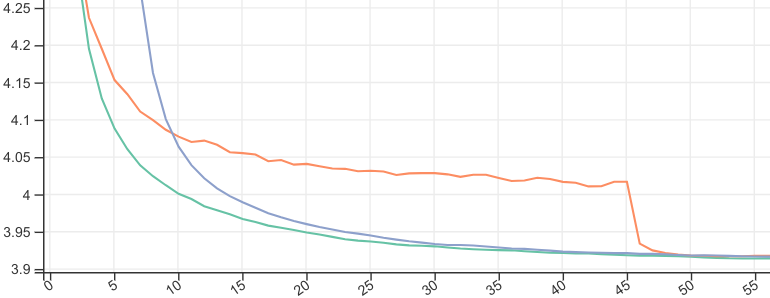
\includegraphics[width=0.9\textwidth]{two-tailed/figure/oswa-vs.png}
  \caption[Validation losses with Two-Tailed Averaging and baselines.]{Validation loss with Two-Tailed Averaging (\tta{}, green), Tail Averaging (TA, orange), and an exponential moving average (EMA, blue) of weights on language modelling on Penn Treebank.
For both TA and EMA, their hyperparameters (the start time and the decay rate) were tuned to minimize the final loss, so it is not a surprise that all three have similar optima.
\tta{} has no hyperparameters and produces much better early solutions.
These two factors make tuning easier and early stopping much more reliable.
Additionally, the noise in the raw loss is effectively smoothed out.
Note that while the \tta{} loss decreases monotonically, gentler and steeper slopes are manifest before and after switch points, respectively.}
  \label{fig:swa-vs-oooswa}
\end{figure}

\begin{figure}[t]
  \centering
  \begin{tikzpicture}
    \node [] at (0,0){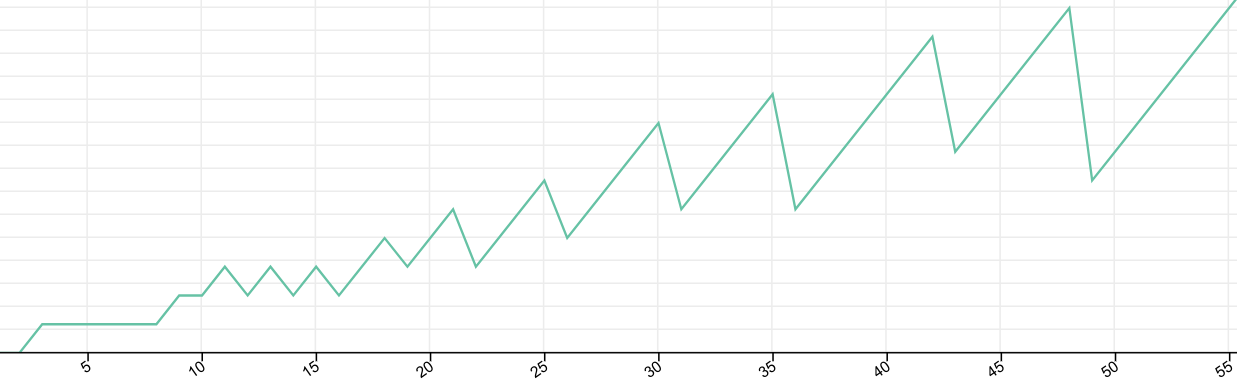
\includegraphics[width=0.9\textwidth]{two-tailed/figure/length.png}};
    \draw [{|[width=1mm]}-Circle,thick](-0.6,-1.66) -- (0.70,-0.105) node[midway,above] {S};
    \draw [-{Circle[open]},thick](0.63,-0.198) -- (1.85,1.33) node[midway,above] {L};
  \end{tikzpicture}
  \caption[Length of the long average ($L$) vs number of evaluations of \tta{}.]{Length of the long average ($L$) vs number of evaluations of \tta{} in \Cref{fig:swa-vs-oooswa}.
Note how the heights of both peaks and valleys increase almost monotonically.
Also, the correspondence between this figure and the schematic in \Cref{fig:schematic} is illustrated on one of the $S$ and $L$ intervals.}
  \label{fig:length}
\end{figure}

Tail Averaging or Stochastic Weight Averaging have been shown previously to be beneficial not only in theory and on simulated data \citep{jain2018parallelizing} but also in language modelling \citep{merity2017regularizing,melis2019mogrifier} and image classification \citep{izmailov2018averaging} experiments.
Hence, in this work we restrict our attention to experiments in a single domain to corroborate the analysis in \Cref{sec:tta-analysis}.
Our goals are to \emph{i)} verify that \tta{} is on par with well-tuned TA and EMA, \emph{ii)} explore the effect of basing the switching logic on the training loss instead of the validation loss, \emph{iii)} demonstrate robustness to the choice of evaluation period, \emph{iv)} and check how well the assumptions made in \Cref{sec:tta-analysis} hold in practice.

In particular, we trained a recurrent language model with several hyperparameters on Penn Treebank \citep{mikolov2010recurrent} using the Rectified Adam optimizer \citep{liu2019variance}, evaluating every 1000 optimization steps.
The hyperparameters were tuned separately for \tta{}, TA \cref{eq:tail-averaging}, and EMA \cref{eq:ema}.
\Cref{fig:swa-vs-oooswa} shows that the final validation losses with all methods are very close, but early losses with \tta{} are much better.
This is expected because TA and EMA are not flexible enough to produce optimal averaging lengths at multiple points along the learning curve despite having an extra hyperparameter.
Conversely, \tta{} has at least one nearly optimal solution between any two subsequent peaks (i.e.\ switch points) in \Cref{fig:length} despite having no hyperparameters.

We also tried the version of the algorithm where the switching logic was based on comparison of the training losses of the short and long averages instead of the validation losses, but the true validation losses were reported.
On this particular language modelling task, the best validation loss with the modified algorithm worsened moderately (3.93 vs 3.92) and was well below the raw validation loss (4.02).
Results on the test set exhibited the same gap.
Since the modified \tta{} was minimizing the training loss, the smoothness of the reported validation losses observed in \Cref{fig:swa-vs-oooswa} were lost in the process.
Similar results were obtained by scheduling a learning rate drop without averaging.

To explore the effect of the evaluation period $E$, we tuned models with four times larger and four times smaller $E$ than in our previously discussed experiments.
As expected, the best final results were very close to each other, with shorter periods having an advantage early in training as the raw loss $F^1$ was more quickly eclipsed by $F^L$.

In addition, we found that the assumptions made in \Cref{sec:tta-analysis} held rather well in practice: the resulting loss $F^L$ in \Cref{fig:swa-vs-oooswa} and the averaging lengths tended to change monotonically (see heights of peaks and valleys in \Cref{fig:length}), making our length-based theoretical results more closely linked to the actual loss.
When that was not the case, we found that the raw loss $F^1$ had started to worsen due to overfitting or, much more rarely, optimization had entered a new basin, violating \Cref{monotone-opt}.
\Cref{fig:overfitting} and \Cref{fig:new-basin} demonstrate the reset heuristic being triggered in these cases.
Finally, TA and \tta{} having almost identical final validation losses weakly supports our assumptions, although a conclusive demonstration would need to plot the results obtained with TA tuned separately for each evaluation.

\begin{figure}[t]
  \centering
  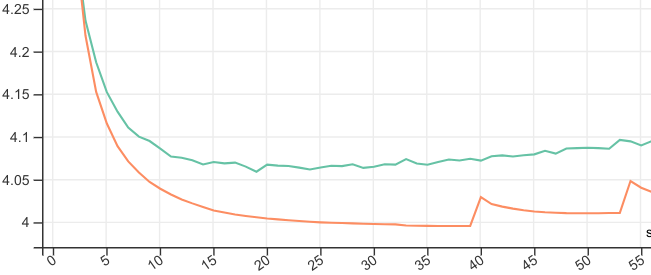
\includegraphics[width=0.9\textwidth]{two-tailed/figure/overfitting.png}
  \caption[Raw and \tta{} validation loss with overfitting.]{Raw (green) and \tta{} (orange) validation loss with overfitting.
The averaged loss bottoms out due to overfitting.
Thus when the averages are reset (twice), the validation loss does not recover.
Although the losses reported after the reset are suboptimal, it does not really matter as a better loss was reported already.}
  \label{fig:overfitting}
\end{figure}

\begin{figure}[t]
  \begin{subfigure}{0.52\textwidth}
    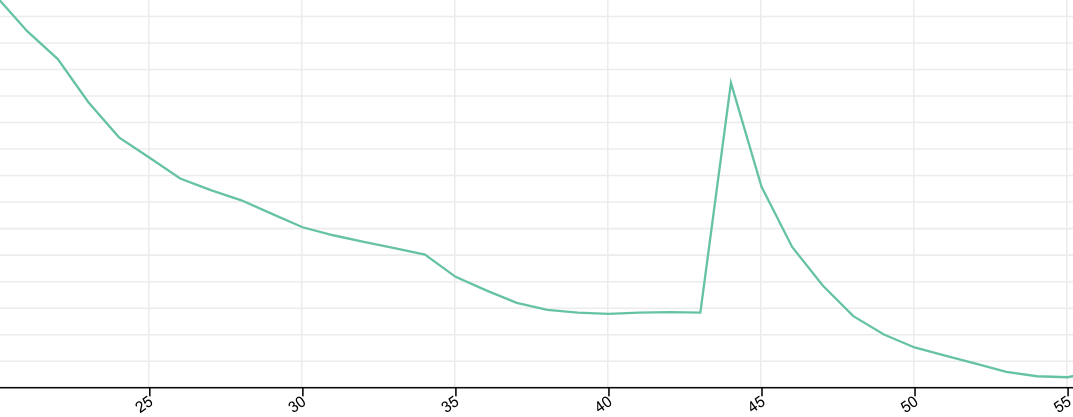
\includegraphics[width=\linewidth,height=2.75cm,clip]{two-tailed/figure/new-basin.png}
    \caption{Validation loss with the long average ($F^L$).}
  \end{subfigure}
  \hfill
  \begin{subfigure}{0.45\textwidth}
    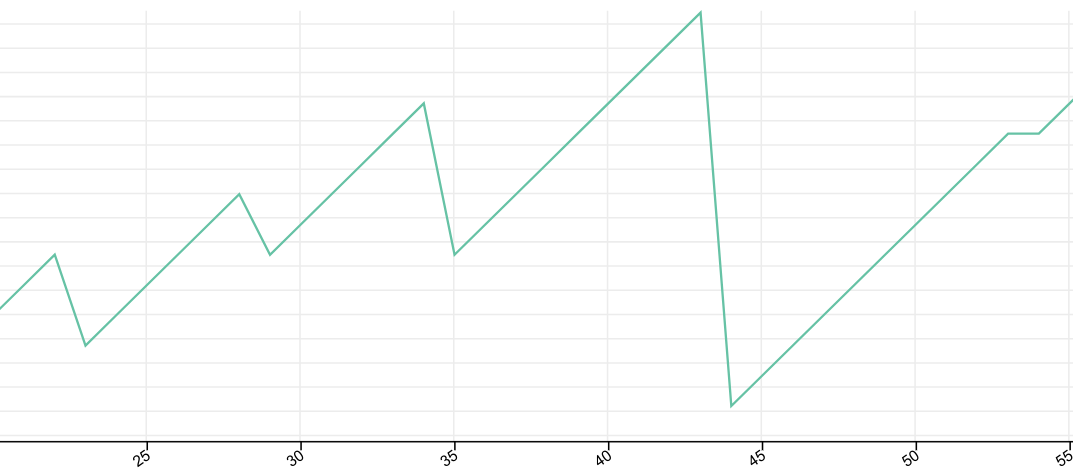
\includegraphics[width=\linewidth,height=2.75cm,clip]
                    {two-tailed/figure/new-basin-samples.png}
    \caption{Length of the long average ($L$).}
  \end{subfigure}
  \caption[Example of optimization entering a new basin.]{Example of optimization entering a new basin.
At $t=40E$ the validation loss bottoms out and starts to slightly worsen.
This is detected at $t=43E$, and both averages are reset.
With the averages now way too short, the loss spikes but then recovers.}
  \label{fig:new-basin}
\end{figure}

\section{Conclusions}

\mglconclusion
Tail averaging improves on Polyak averaging's non-asymptotic behaviour by excluding a number of leading iterates of stochastic optimization from its calculations.
In practice, with a finite number of optimization steps and a learning rate that cannot be annealed to zero, Tail Averaging can get much closer to a local minimum point of the training loss than either the individual iterates or the Polyak average.
However, the number of leading iterates to ignore is an important hyperparameter, and starting averaging too early or too late leads to inefficient use of resources or suboptimal solutions.
Our work focussed on improving generalization, which makes setting this hyperparameter even more difficult, especially in the presence of other hyperparameters and overfitting.
Furthermore, before averaging starts, the loss is only weakly informative of the final performance, which makes early stopping unreliable.
To alleviate these problems, we propose an anytime variant of Tail Averaging intended for improving generalization not pure optimization that has no hyperparameters and approximates the optimal tail at all optimization steps.
Our algorithm is based on two running averages with adaptive lengths bounded in terms of the optimal tail length, one of which achieves approximate optimality with some regularity.

In summary, we presented a variant of Tail Averaging and Stochastic Weight Averaging based on two running averages.
Compared to them, Two-Tailed Averaging requires additional storage for the second running average and relies on periodic evaluation of generalization performance.
In return, \tta{} removes a hyperparameter and provides an estimate of the optimal tail at all optimization steps.
This makes hyperparameter tuning easier and early evaluation more representative of final performance, allowing it to support early and anytime stopping better.
Owing to its simplicity, low implementation cost and adaptivity, \tta{} is a practical and widely applicable method for improving generalization.

Looking beyond the scope of this work, exploring the relationship between iterate averaging and learning rate schedules is a promising direction as existing \citep{merity2017regularizing} and our own limited experimental results indicate that dropping the learning rate and Tail Averaging perform comparably.
The properties of our algorithm are particularly compelling for continual learning: by allowing the learning rate to remain high and being able to adapt the averaging length to changing circumstances, \tta{} lets the model maintain high plasticity while reaping the benefits of averaging.

In addition, averaging weights can be viewed as a cheap approximation to averaging predictions when the averaged weights reside in a region with a suitable geometry.
The combination of averaging weights within such regions and averaging predictions over regions (each with its own weight average) could potentially achieve a better loss than weight averaging alone at much lower storage and evaluation cost than pure prediction averaging.
We leave these avenues for future work to explore.

\mglsep



\chapter{Refining Recurrences}
\label{sec:refining-recurrences}

\mglepigraph{0.79}{The proverbial German phenomenon of the “verb-at-the-end”, about which droll tales of absentminded professors who would begin a sentence, ramble on for an entire lecture, and then finish up by rattling off a string of verbs by which their audience, for whom the stack had long since lost its coherence, would be totally nonplussed, are told, is an excellent example of linguistic recursion.}{Douglas Hofstadter}
\mgllettrine{findent=-1.0em,nindent=0.8em,slope=0.8em}{R}{eliable model}
comparison is crucial for continued innovation in language modelling.
With so much attention on Transformers \citep{vaswani2017attention}, the development of purely recurrent models has ebbed away.
It might be tempting to claim that purely recurrent models are fundamentally worse models of language than attention-based ones, but they seem to have an edge on small datasets, while on larger datasets their lack of scalability on current hardware \citep{DBLP:journals/corr/abs-2009-06489} also plays an important role in their evaluation.
Due to being unfashionable and slow, their fitness might be underestimated especially on all but the smallest datasets with the exception of S4 \citep{gu2021efficiently}, a highly parallelizable, long-range model.
The purpose of this work is simply to apply more resources to advancing and evaluating recurrent models --~despite, and to compensate for, their computational inefficiency~-- to better represent their performance in future model comparisons.

Starting from the Mogrifier LSTM \citep{melis2019mogrifier}, a state-of-the-art recurrent language model, we introduce several small changes, which involve not only the design of the recurrent cell but the overall architecture, the training objective, and optimization.
On all datasets, these changes combine to a significant, and in some cases large, effect.


\section{Rewired LSTM}

We propose a novel recurrent cell, a slightly tweaked version of the LSTM \citep{hochreiter1997lstm}, as presented in \eqref{eq:lstm}.
To recap, with $m$ and $n$ being the sizes of the input and the cell state, let the $\LSTM \colon \mathbb{R}^n\times\mathbb{R}^n \times \mathbb{R}^m \to \mathbb{R}^n \times \mathbb{R}^n$ be a function that computes the updated state $\vc$ and output $\vh$ from the previous state $\vcprev$, output $\vhprev$ and the current input $\vx$.
Concretely, $\LSTM(\vcprev, \vhprev, \vx) = (\vc, \vh)$, where
{\setlength{\jot}{0.5em}
\begin{align*}
  \vi &= \sigma\bigl(\mW^{ix} \vx + \mW^{ih} \vhprev + \vb^i\bigr)\\
  \vj &= \tanh(\mW^{jx}\vx + \mW^{jh} \vhprev + \vb^j) \\
  \vf &= \sigma(\mW^{fx} \textcolor{mglblue}{\vx} + \mW^{fh} \vhprev + \vb^f) \\
  \vc &= \vf \odot \vcprev + \textcolor{mglgreen}{\vi} \odot \vj \\
  \vo &= \sigma(\textcolor{mglred}{\mW^{ox} \vx + \mW^{oh} \vhprev} + \vb^o) \\
  \vh &= \vo \odot \tanh(\vc).
\end{align*}}%
In the above, $\sigma$ is the logistic sigmoid function, $\odot$ is the elementwise product, $\mW^{**}$ and $\vb^{*}$ are weight matrices and biases.
As in \Cref{fig:lstm}, the parts altered by the RLSTM (see \Cref{fig:rlstm}) are colour coded.

To accommodate the performance characteristics of parallel hardware, the activations of $\vi$, $\vj$, $\vf$, $\vo$ are in practice often computed by tiling the eight $\mW^{**}$ into one large matrix and multiplying it with the concatenated input and recurrent state $[\vx, \vhprev]$.

\begin{figure}[!t]\centering
\begin{tikzpicture}[
    % GLOBAL CFG
    font=\sf \scriptsize,
    >=LaTeX,
    % Styles
    cell/.style={% For the main box
        rectangle,
        rounded corners=5mm,
        draw,
        very thick,
        },
    operator/.style={%For operators like +  and  x
        circle,
        draw,
        inner sep=-0.5pt,
        minimum height =.2cm,
        },
    function/.style={%For functions
        ellipse,
        draw,
        inner sep=1pt
        },
    ct/.style={% For external inputs and outputs
        circle,
        draw,
        line width = .75pt,
        minimum width=0.75cm,
        inner sep=1pt,
        },
    gt/.style={% For internal inputs
        rectangle,
        draw,
        minimum width=4mm,
        minimum height=3mm,
        inner sep=1pt
        },
    mylabel/.style={% something new that I have learned
        font=\scriptsize\sffamily
        },
    ArrowC1/.style={% Arrows with rounded corners
        rounded corners=.20cm,
        thick,
        },
    ArrowC2/.style={% Arrows with big rounded corners
        rounded corners=.5cm,
        thick,
        },
    ]

%Start drawing the thing...
    % Draw the cell:
    \node [cell, minimum height =4.5cm, minimum width=7cm] at (-0.50,0.25){} ;

    % Draw inputs named ibox#
    \node [gt] (ibox1) at (-2.5,0.75) {$\sigma$};
    \node [gt] (ibox2) at (-1.5,-0.75) {$\sigma$};
    \node [gt, minimum width=0.75cm] (ibox3) at (-0.5,-0.75) {tanh};
    \node [gt] (ibox4) at (0.5,-0.75) {$\sigma$};

   % Draw opérators   named mux# , add# and func#
    \node [operator] (mux1) at (-2.5,2.0) {\dotinnode};
    \node [operator] (add1) at (-0.5,2.0) {$+$};
    \node [operator] (mux2) at (-0.5,1.25) {\dotinnode};
    \node [operator] (mux3) at (1.5,0) {\dotinnode};
    \node [function] (func1) at (1.5,0.75) {tanh};

    % Draw External inputs? named as basis c,h,x
    \node[ct, label={[mylabel,align=center]Prev.\\State}] (c) at (-5.0,2.0) {$\vcprev$};
    \node[ct, label={[mylabel,align=center]Prev.\\Output}] (h) at (-5.0,-1.5) {$\vhprev$};
    \node[ct, label={[mylabel]left:Input}] (x) at (-3.25,-3) {$\vx$};

    % Draw External outputs? named as basis c2,h2,x2
    \node[ct, label={[mylabel]State}] (c2) at (4,2.0) {$\vc$};
    \node[ct, label={[mylabel]Output}] (h2) at (4,-1.5) {$\vh$};
    \node[ct, label={[mylabel]left:Output}] (x2) at (2.5,3.5) {$\vh$};

% Start connecting all.
    %Intersections and displacements are used.
    % Drawing arrows
    \draw [ArrowC2] (h) -- ++(2,0);
    \draw [ArrowC2,mglred] (h)++(2,0) -| (ibox4);
    \draw [ArrowC1] (c) -- (mux1) -- (add1) -- (c2);

    % Inputs
    \draw [ArrowC1,mglblue] (x) -- (x |- h)-| (ibox3);
    \draw [ArrowC1] (h -| ibox1)++(-1.5,0) -| (ibox1);
    \draw [ArrowC1] (h -| ibox2)++(-1.5,0) -| (ibox2);
    \draw [ArrowC1] (h -| ibox3)++(-1.5,0) -| (ibox3);

    % Internal
    \draw [->, ArrowC2] (ibox1) -- (mux1) node[pos=0.4,left] {$f$};
    \draw [->, ArrowC2,mglgreen] (ibox2) |- (mux2) node[pos=0.1, left, text=black] {$i$};
    \draw [->, ArrowC1] (ibox3) -- (mux2) node[pos=0.2, left] {$j$};
    \draw [->, ArrowC2] (ibox4) |- (mux3) node[midway] {$o$};

    \draw [->, ArrowC1] (mux2) -- (add1);
    \draw [->, ArrowC1] (add1 -| func1)++(-0.5,0) -| (func1);
    \draw [->, ArrowC2] (func1) -- (mux3);

    %Outputs
    \draw [-, ArrowC2] (mux3) |- (h2);
    \draw (c2 -| x2) ++(0,-0.1) coordinate (i1);
    \draw [-, ArrowC2] (h2 -| x2)++(-0.5,0) -| (i1);
    \draw [-, ArrowC2] (i1)++(0,0.2) -- (x2);

\end{tikzpicture}
\caption{Schematic of the LSTM cell in the style of \url{https://colah.github.io/posts/2015-08-Understanding-LSTMs/}.
All gates are computed from $\vhprev$ and $\vx$.
Differences from the RLSTM cell are colour coded to ease comparison to \Cref{fig:rlstm}.}
\label{fig:lstm}
\end{figure}

\begin{figure}[!t]\centering
\begin{tikzpicture}[
    % GLOBAL CFG
    font=\sf \scriptsize,
    >=LaTeX,
    % Styles
    cell/.style={% For the main box
        rectangle,
        rounded corners=5mm,
        draw,
        very thick,
        },
    operator/.style={%For operators like +  and  x
        circle,
        draw,
        inner sep=-0.5pt,
        minimum height =.2cm,
        },
    function/.style={%For functions
        ellipse,
        draw,
        inner sep=1pt
        },
    ct/.style={% For external inputs and outputs
        circle,
        draw,
        line width = .75pt,
        minimum width=0.75cm,
        inner sep=1pt,
        },
    gt/.style={% For internal inputs
        rectangle,
        draw,
        minimum width=4mm,
        minimum height=3mm,
        inner sep=1pt
        },
    mylabel/.style={% something new that I have learned
        font=\scriptsize\sffamily
        },
    ArrowC1/.style={% Arrows with rounded corners
        rounded corners=.20cm,
        thick,
        },
    ArrowC2/.style={% Arrows with big rounded corners
        rounded corners=.5cm,
        thick,
        },
    ]

%Start drawing the thing...
    % Draw the cell:
    \node [cell, minimum height =4.5cm, minimum width=7cm] at (-0.50,0.25){} ;

    % Draw inputs named ibox#
    \node [gt] (ibox1) at (-2.5,0.75) {$\sigma$};
    \node [gt] (ibox2) at (-1.5,-0.75) {$\sigma$};
    \node [gt, minimum width=0.75cm] (ibox3) at (-0.5,-0.75) {tanh};
    \node [gt] (ibox4) at (0.5,0.75) {$\sigma$};

   % Draw opérators   named mux# , add# and func#
    \node [function,mglgreen] (cap) at (-1.5,1.25) {min};
    \node [operator] (capped) at (-0.5,1.25) {\dotinnode};
    \node [operator] (mux1) at (-2.5,2.0) {\dotinnode};
    \node [operator] (add1) at (-0.5,2.0) {$+$};
    \node [operator,mglblue] (mux2) at (-1.0,0) {\dotinnode};
    \node [operator] (mux3) at (1.5,0) {\dotinnode};
    \node [function] (func1) at (1.5,0.75) {tanh};

    % Draw External inputs? named as basis c,h,x
    \node[ct, label={[mylabel,align=center]Prev.\\State}] (c) at (-5.0,2.0) {$\vcprev$};
    \node[ct, label={[mylabel,align=center]Prev.\\Output}] (h) at (-5.0,-1.5) {$\vhprev$};
    \node[ct, label={[mylabel]left:Input}] (x) at (-2.25,-3) {$\vx$};

    % Draw External outputs? named as basis c2,h2,x2
    \node[ct, label={[mylabel]State}] (c2) at (4,2.0) {$\vc$};
    \node[ct, label={[mylabel]Output}] (h2) at (4,-1.5) {$\vh$};
    \node[ct, label={[mylabel]left:Output}] (x2) at (2.5,3.5) {$\vh$};

% Start connecting all.
    %Intersections and displacements are used.
    % Drawing arrows
    \draw [ArrowC1,mglred] (add1) -| (ibox4);
    \draw [ArrowC1] (c) -- (mux1) -- (add1) -- (c2);

    % Inputs
    \draw [ArrowC1,mglblue] (x) -- (x |- h)-| (ibox2);
    \draw [ArrowC1] (h) -| (ibox1);
    \draw [ArrowC1] (h -| ibox2)++(-1.5,0) -| (ibox2);
    \draw [ArrowC2] (h -| ibox3)++(-1.5,0) -| (ibox3);

    % Internal
    \draw [->, ArrowC2] (ibox1) -- (mux1) node[pos=0.4,left] {$f$};
    \draw [->, ArrowC2] (ibox4) |- (mux3) node[midway] {$o$};
    \draw [->, ArrowC1,mglgreen] (ibox1) |- (cap) node[midway, above right] {$1\!-\!f$};

    \draw [-, ArrowC1,mglgreen] (ibox2) |- (-1.5,0.075);
    \draw [->, ArrowC1,mglgreen] (-1.5,0.375)++(0,0.1) -- (cap);

    \draw [->, ArrowC1,mglgreen] (cap) -- (capped);
    \draw [->, ArrowC1] (ibox3) -- (capped);
    \draw [->, ArrowC2] (capped) -- (add1);
    \draw [-, ArrowC1,mglblue] (mux2) |- (-1.5,0.375) -| (ibox1);
    \draw [->, ArrowC1] (add1 -| func1)++(-0.5,0) -| (func1);
    \draw [->, ArrowC2] (func1) -- (mux3);
    \draw [->, ArrowC1,mglblue] (ibox2) |- (mux2) node[pos=0.2, left, text=black] {$i$};
    \draw [->, ArrowC1,mglblue] (ibox3) |- (mux2) node[pos=0.2, left, text=black] {$j$};

    %Outputs
    \draw [-, ArrowC2] (mux3) |- (h2);
    \draw (c2 -| x2) ++(0,-0.1) coordinate (i1);
    \draw [-, ArrowC2] (h2 -| x2)++(-0.5,0) -| (i1);
    \draw [-, ArrowC2] (i1)++(0,0.2) -- (x2);

\end{tikzpicture}
\caption{Schematic of the RLSTM cell.
1. The forget gate \textcolor{mglblue}{$\vf$} is computed from \textcolor{mglblue}{$\vi\odot \vj$}, 2. \textcolor{mglgreen}{$\vi$} is capped at \textcolor{mglgreen}{$1-\vf$}, 3. \textcolor{mglred}{$\vo$} is computed from \textcolor{mglred}{$\vc$}.
There is an apparent loss of parallelization opportunities due to the increased depth of the computation graph.}
\label{fig:rlstm}
\end{figure}

Intuitively, in $\vc = \vf \odot \vcprev + \vi \odot \vj$ the forget gate $\vf$ and the proposed update $\vi \odot \vj$ depend on each other, and computing them in parallel from the same inputs may be partially redundant.
On the flipside, the parametrization of the proposed update as a product is more expressive than that of the forget gate, so the overall cell update may lose some of the extra expressivity.
Hence, it makes sense to compute the forget gate from the proposed update instead.
Note that this reduces the opportunities for parallelization and makes cell updates slower.

Further disregarding efficiency on today's hardware, to reduce parameter count and to encourage storing more information in the cell state $\mathbf{c}$, we compute $\vo$ from $\mathbf{c}$, dropping a potential bypass connection from $\vx$ to $\vh$.
Finally, to make exploding gradients less likely, we cap $\vi$ at $\mathbf{1-f}$ to ensure $|c_u| \leqslant 1$ for all memory units $u$.
The update of our Rewired LSTM (RLSTM) cell takes the form
{\setlength{\jot}{0.5em}
\begin{align*}
  \vi &= \sigma\bigl(\mW^{ix} \vx + \mW^{ih} \vhprev + \vb^i\bigr) \\
  \vj &= \tanh\bigl(\mW^{jx}\vx + \mW^{jh} \vhprev + \vb^j\bigr) \\
  \vf &= \sigma\bigl(\mW^{fu} \textcolor{mglblue}{\vi\odot \vj} + \mW^{fh} \vhprev + \vb^f\bigr) \\
  \vc &= \vf \odot \vcprev + \textcolor{mglgreen}{\min(\vi, 1-\vf)} \odot \vj \\
  \vo &= \sigma\bigl(\textcolor{mglred}{\mW^{oc} \vc} + \vb^o\bigr) \\
  \vh &= \vo \odot \tanh\bigl(\vc\bigr),
\end{align*}}%
where the changes from the LSTM are coloured.
Based on this altered computation, we define the $\RLSTM$ function similarly to the $\LSTM$ above.

\section{Architecture}
\label{sec:architecture}

The way recurrent cells are combined can also be improved.
Here, we opt to use residual connections, where previous works have used stacked LSTMs \citep{merity2017regularizing} or skip connections \citep{melis2019mogrifier}, which feed directly into the final output.
Along with this change, we apply dropout \citep{hinton2012improving} to the cell output before it is added to the residual branch.

%% To describe the overall architecture more formally, let us denote the mogrification operation \citep{melis2019mogrifier} with the following $\mathbb{R}^n\times\mathbb{R}^m \to \mathbb{R}^n \times \mathbb{R}^m$ function:
%% \begin{align*}
%%   \mogrify(\vh,\vx) &= \vh^{2\floor{r/2}}, \vx^{2\floor{(r+1)/2}-1} \\
%%   \vx^{-1}, \vh^0 &= \vx, \vh \\
%%   \vx^i &= 2\sigma\bigl(\mQ^{i}\vh^{i-1}\bigr) \odot \vx^{i-2}, &
%%   \text{for odd i} \in [1..r]\\
%%   \vh^i &= 2\sigma\bigl(\mR^{i}\vx^{i-1}\bigr) \odot \vh^{i-2},
%%   & \text{for even i} \in [1..r]
%% \end{align*}
%% where the number of rounds $r$ is a hyperparameter, and $\mQ^{i} \in \mathbb{R}^{m\times n}, \mR^{i} \in \mathbb{R}^{n\times m}$ are (possibly low-rank factorized) weight matrices.

To describe the overall architecture more formally, with time steps $t \in [1, 2, \dots]$ and layers $l \in [1..L]$, from the vector of token indices $\vw$  in a fixed vocabulary, the probability distribution of the next token $p(.\tmid \vw_{<t},\mM_t)$ is computed as
{\setlength{\jot}{0.6em}
\begin{align*}
\vc^l_0, \vh^l_0 &= \mathbf{0}, \mathbf{0}\\
% Kerning is funny, probably due to lining figures. Add some negative kerns.
\hat{\vx}^0_t\! &= \onehot\bigl(\vw_t\bigr) \mE^{\textrm{in}} \odot \mM^\textrm{in}_t\\
\hat{\vx}^l_t &= \vh^l_t \odot \mM^{\textrm{cell},l}_t & (l > 1) \\
\hat{\vh}^l_t &= \vh^l_t \odot \mM^{\textrm{state},l}\\
\vc^1_t\!, \vh^1_t\! &= \textrm{[R]LSTM}\Bigl(\vc^0_{t-1}, \mogrify\Bigl(\hat{\vh}^1_{t-1}, \hat{\vx}^0_t\Bigr)\Bigr) \\
\vc^l_t, \vh^l_t &= \textrm{[R]LSTM}\Bigl(\vc^l_{t-1}, \mogrify\Bigl(\hat{\vh}^l_{t-1}, \sum\nolimits_{i=1}^{l-1} \hat{\vx}^i_t\Bigr)\Bigr) \\
p(.\tmid \vw_{<t},\mM_t) &= \softmax\Bigl(\Bigl(\sum\nolimits_{l=1}^L \hat{\vx}^l_t\Bigr) \odot \mM^{\textrm{out}}_t \mE^{\textrm{out}} + \vb^{\textrm{out}}\Bigr),
\end{align*}}%
where we assume that $m=n$ to allow for a residual architecture without projections and use the \emph{mogrify} function as defined in \eqref{eq:mogrify}.
$\mE^{\textrm{in}}$ and $\mE^{\textrm{out}}$ are the input and output embedding matrices.
For word-based language modelling, we set $\mE^{\textrm{out}}$ to the transpose of $\mE^{\textrm{in}}$ \citep{DBLP:journals/corr/ZophL16,DBLP:journals/corr/PressW16}.
$\mM_t$ is the set of individual input, cell, state and output dropout mask matrices $\mM^{\textrm{in}}_t$, $\mM^{\textrm{cell},l}_t$, $\mM^{\textrm{state},l}$ and $\mM^{\textrm{out}}_t$.
Note that for state dropout, we use the variational dropout of \citet{gal2016theoretically}, thus $\mM^{\textrm{state},l}$ does not depend on $t$.
In addition, when an RLSTM is used instead of an LSTM cell, we also apply the state dropout mask to $\vc$ in the calculation of $\vo = \sigma(\mW^{oc} (\vc \odot \mM^{\textrm{state},l}) + \vb^o)$.% of the corresponding layers.


\section{Objective}

In the objective, we average model predictions over multiple dropout samples:
\begin{align*}
\ln p\condp[\big]{\vw_t}{\vw_{<t}} = \ln\biggl(\frac{1}{D} \sum_{d=1}^D p\condp[\Big]{\vw_t}{\vw_{<t},\mM^d_t}\biggr),
\end{align*}
where $D$ is the number of samples taken.
As pointed out by \citet{noh2017regularizing}, when dropout is interpreted as optimizing a variational lower bound on the log likelihood \citep{gal2016theoretically}, this procedure is an instantiation of Importance Weighted Autoencoders \citep{burda2015importance}, which provide a bound tighter than the single-sample ELBO.

\section{Optimization}

To increase the stability of optimization and allow slightly higher learning rates, we use Rectified Adam \citep{liu2019variance}.
If training diverges, we reset the weights and the optimization state to the previous best checkpoint and multiply the learning rate by 0.9.

\citet{merity2017regularizing} switch to averaging weights at a late stage of optimization when the validation loss has not decreased for a while.
A similar procedure, called Stochastic Weight Averaging (SWA), was also proposed \citep{izmailov2018averaging}, and corresponding theory was developed in \citet{jain2018parallelizing} under the name of Tail Averaging.
Here, we employ Two-Tailed Averaging \citep{https://doi.org/10.48550/arxiv.2209.12581}, which has no hyperparameters and provides a good approximation to the optimal weight average at every step of optimization.
Two-Tailed Averaging (\tta{}) thus requires no tuning and is a much better fit with early stopping, which is what we do on \enwik and \texteight \citep{hutter2012human}.
While easier to work with, \tta{} does not improve the final results over well-tuned Tail Averaging, which is also used by our baseline, the Mogrifier LSTM.

LSTM and RLSTM forget gates are initialized with Chrono init \citep{tallec2018can} as $\vb^f \sim \ln(\mathcal{U}(1, T_\text{max}-1))$, where $T_\text{max}$ is a tuned hyperparameter.
Finally, we just train models longer where it is beneficial.

\section{Dynamic Evaluation}

\citet{hinton1987using} proposed fast weights, wherein parameters have a slow- and a fast-changing component.
Much later, \citet{ba2016using} showed a form of attention to be an instantiation of fast weights.
Similarly, some forms of meta learning, e.g.\ few-shot adaptation with gradient updates, can be interpreted as fast weights.
To mimic this setting and gain a particularly general fast weights implementation, it would be desirable to allow the model weights to depend on the context as in $p(x_i\tmid \theta(x_{<i}),x_{<i})$, where the fast weights $\theta(x_{<i})$ are computed with gradient-based updates to the slow weights $\theta_0$.
However, due to the practical difficulties involved in training batches with per-example inner gradient updates, we eschew fast weights at training time but not when performing evaluation, thus we end up with what is called dynamic evaluation \citep{krause2017dynamic}.
Here, we present dynamic evaluation results as a proxy for the gradient-based fast weights model.

As argued heuristically above, attention may be interpreted as a particular way of adapting the weights to the context (outer product memory), like the Mogrifier, which has an even more restricted form of update (scaling columns of weight matrices).
Thus, it is not surprising that \citet{melis2019mogrifier} found that Transformers are better at adapting without changing their weights, leaving less in-context signal for dynamic evaluation to pick up.

\section{Experimental Setup}

We follow the experimental setup of our baseline \citep{melis2019mogrifier}.
In the following, we list only the most pertinent choices in our experimental setup; everything else is the same as in the baseline.
Note that the baseline's and our LSTM implementation already includes the capped input gate ($\min(1-\vf,\vi)$) of the RLSTM.
For the black-box hyperparameter tuner \citep{golovin2017google}, due to the switch to a residual architecture, the baseline's \emph{inter\_layer\_dropout} hyperparameter is replaced with \emph{cell\_output\_dropout} (see $\mM^{\textrm{cell},l}$ in \Cref{sec:architecture}).
In addition, the top of the Chrono init range $T_{\textit{max}}$ is a new hyperparameter from the $[e^2,e^5]$ range.

For word-level language modelling on Penn Treebank \citep{marcus1993building} with preprocessing by \citep{mikolov2010recurrent}, we trained 2-layer models for about 400 epochs with 8 dropout samples.
Batch size was 128, and we trained with a BPTT \citep{werbos1990backpropagation} window size of 70.
Experiments on \wikitexttwo \citep{DBLP:journals/corr/MerityXBS16} were conducted similarly, with the exception of training for 250 epochs and using 4 dropout samples.

For character-based language modelling on Penn Treebank, we trained 2-layer models for 100 epochs with 4 dropout samples, batch size 128, and a BPTT window size of 200.
On \enwik and \texteight \citep{hutter2012human}, we trained 6-layer models for 200 epochs, whereas the baseline model had 4 layers and was trained for only 29 epochs.
Batch size was 128, and the BPTT window size was set to 256.
Increasing the window size had no discernible effect in agreement with the findings of \citet{khandelwal2018sharp}.
Due to the long time required to train these models, the best hyperparameters were selected from a random pool of 60 candidates.
Since preliminary experiments indicated that the benefit of using multiple dropout samples was less than 0.01 bpc, we refrained from using more than one dropout sample to save time.

Model evaluation was performed with the standard, deterministic dropout; we refrained from using the more expensive Monte Carlo averaging \citep{gal2016theoretically}.
The optimal softmax temperature was selected at evaluation time to maximize the validation log-likelihood \citep{melis2018pushing}.
Finally, we report results with and without dynamic evaluation \citep{krause2017dynamic}.


\section{Results}

Due to the aforementioned loss of parallelization opportunities, we found that the RLSTM was about 10\%--30\% slower than the LSTM on NVIDIA p100 GPUs.
Still, the RLSTM retained a significant advantage over the LSTM even when trained for the same wall clock time.

\begin{table}
  \setlength{\abovecaptionskip}{0.2\baselineskip}
  \caption[Word-level perplexities of near state-of-the-art models.]{Word-level perplexities of near state-of-the-art models.
Names for models with our new results are in bold.
On \wikitexttwo, the baseline employed Mixture of Softmaxes \citep{yang2017improved}, but we found no benefit to that when used in conjunction with multiple dropout samples.}
  \label{tab:cb-word-results}

  \centering
  \small
  \begin{tabular}{@{}llrlrlr@{}}
    & & & \multicolumn{2}{c}{No Dyneval} & \multicolumn{2}{c}{Dyneval} \\
    \cmidrule(lr){4-5} \cmidrule(l){6-7}
    & & & Val. & Test & Val. & Test \\
    \midrule
    \parbox[t]{5mm}{\multirow{4}{*}{\rotatebox[origin=c]{90}{PTB}}}
    & Transformer-XL \citep{dai2019transformer} & 24M
        & 56.7 & 54.5 & & \\
    & Mogrifier LSTM \citep{melis2019mogrifier} & 24M
        & \nlltoppl{3.95346} & \nlltoppl{3.93124}
        & \nlltoppl{3.80963} & \nlltoppl{3.80708} \\
    & \textbf{Mogrifier LSTM} & 24M
        & \nlltoppl{3.91065} & \nlltoppl{3.88170}
        & \nlltoppl{3.77302} & \nlltoppl{3.76763} \\
    & \textbf{Mogrifier RLSTM} & 24M
        & \nlltoppl{3.88915} & \nlltopplbold{3.86939}
        & \nlltoppl{3.75818} & \nlltopplbold{3.75805} \\
    \midrule
    \parbox[t]{5mm}{\multirow{3}{*}{\rotatebox[origin=c]{90}{WT$2$}}}
    & Mogrifier LSTM MoS$2$ & 35M
        & \nlltoppl{4.07235} & \nlltoppl{4.03665}
        & \nlltoppl{3.70429} & \nlltoppl{3.66475} \\
    & \textbf{Mogrifier LSTM} & 35M
        & \nlltoppl{4.05079} & \nlltoppl{4.02249}
        & \nlltoppl{3.68904} & \nlltoppl{3.65259} \\
    & \textbf{Mogrifier RLSTM} & 35M
        & \nlltoppl{4.03738} & \nlltopplbold{4.00680}
        & \nlltoppl{3.67189} & \nlltopplbold{3.63711} \\
    \midrule
  \end{tabular}
\end{table}

On word-level language modelling (see \Cref{tab:cb-word-results}), only training for half the epochs, our Mogrifier LSTM outperformed the same model in \citet{melis2019mogrifier}, the baseline.
This was mostly due to the quicker convergence with multiple dropout samples and, to a small degree, to the initialization of the forget gate.
Note that on 2-layer models, which we used on this task, residual connections are identical to skip connections, which are employed by the baseline.
On top of these improvements, the RLSTM outperformed the LSTM by a small margin, and we established a new state of the art on both datasets with and without dynamic evaluation.

\begin{table}
  \setlength{\abovecaptionskip}{0.2\baselineskip}
  \caption[Bits per character on character-based datasets of near state-of-the-art models.]{Bits per character on character-based datasets of near state-of-the-art models.
Names for models with our new results are in bold.
The best test results with and without dynamic evaluation for a given dataset and model size are in bold unless there is a smaller model with a better result.}
  \label{tab:cb-character-results}

  \centering
  \small
  \begin{tabular}{@{}llrllll@{}}
    & & & \multicolumn{2}{c}{No Dyneval} & \multicolumn{2}{c}{Dyneval} \\
    \cmidrule(lr){4-5} \cmidrule(lr){6-7}
    & & & Val. & \multicolumn{1}{r}{Test} & Val. & \multicolumn{1}{r}{Test} \\
    \midrule
    \parbox[t]{5mm}{\multirow{3}{*}{\rotatebox[origin=c]{90}{PTB}}}
    & Mogrifier LSTM \citep{melis2019mogrifier} & 24M
        & \nlltobpc{0.79616} & \nlltobpc{0.78415}
        & \nlltobpc{0.76119} & \nlltobpc{0.75439} \\
    & \textbf{Mogrifier LSTM} & 24M
        & \nlltobpc{0.78156} & \nlltobpc{0.76895}
        & \nlltobpc{0.75215} & \nlltobpc{0.74422} \\
    & \textbf{Mogrifier RLSTM} & 24M
        & \nlltobpc{0.77313} & \nlltobpcbold{0.75999}
        & \nlltobpc{0.74369} & \nlltobpcbold{0.73561} \\

    \midrule
    \parbox[t]{5mm}{\multirow{12}{*}{\rotatebox[origin=c]{90}{\enwik}}}
    & Transformer-XL (d24) \citep{dai2019transformer} & 277M
        & & 0.993 & & 0.940 \\
    & Longformer \citep{beltagy2020longformer} & 277M
        & & \textbf{0.97} & & \\
    \cmidrule(l){2-7}
    & Transformer-XL (d18) \citep{dai2019transformer} & 88M
        & & 1.03 & & \\
    & Longformer \citep{beltagy2020longformer} & 102M
        & & \textbf{0.99} & & \\
    & Mogrifier LSTM \citep{melis2019mogrifier} & 96M
        & \nlltobpc{0.76935} & \nlltobpc{0.77792}
        & \nlltobpc{0.69911} & \nlltobpc{0.68516} \\
    & \textbf{Mogrifier LSTM} & 96M
        & \nlltobpc{0.73297} & \nlltobpc{0.74346}
        & \nlltobpc{0.66784} & \nlltobpc{0.65592} \\
    & \textbf{Mogrifier RLSTM} & 96M
        & \nlltobpc{0.71288} & \nlltobpc{0.72236}
        & \nlltobpc{0.65992} & \nlltobpcbold{0.64803} \\
    \cmidrule(l){2-7}
    & Transformer-XL (d12) \citep{dai2019transformer} & 41M
        & & 1.06 & & 1.01 \\
    & Longformer \citep{beltagy2020longformer} & 41M
        & 1.02 & \textbf{1.00} & & \\
    & Mogrifier LSTM \citep{melis2019mogrifier}& 48M
        & \nlltobpc{0.78663} & \nlltobpc{0.79413}
        & \nlltobpc{0.71751} & \nlltobpc{0.70177} \\
    & \textbf{Mogrifier LSTM} & 48M
        & \nlltobpc{0.75051} & \nlltobpc{0.75813}
        & \nlltobpc{0.68495} & \nlltobpc{0.67213} \\
    & \textbf{Mogrifier RLSTM} & 48M
        & \nlltobpc{0.73502} & \nlltobpc{0.74228}
        & \nlltobpc{0.68362} & \nlltobpcbold{0.67110} \\

    \midrule
    \parbox[t]{5mm}{\multirow{6}{*}{\rotatebox[origin=c]{90}{\texteight}}}
    & Transformer-XL (d24) \citep{dai2019transformer} & 277M
        & & \textbf{1.08} & & \textbf{1.038} \\
    \cmidrule(l){2-7}
    & \textbf{Mogrifier LSTM} & 96M
        & \nlltobpc{0.71598} & \nlltobpc{0.76681}
        & \nlltobpc{0.67725} &  \nlltobpc{0.72559} \\
    & \textbf{Mogrifier RLSTM} & 96M
        & \nlltobpc{0.70855} & \nlltobpc{0.75983}
        & \nlltobpc{0.67595} & \nlltobpc{0.72363} \\
    \cmidrule(l){2-7}
    & Longformer \citep{beltagy2020longformer} & 41M
        & 1.04 & \textbf{1.10} & & \\
    & \textbf{Mogrifier LSTM} & 48M
        & \nlltobpc{0.73670} & \nlltobpc{0.79002}
        & \nlltobpc{0.69642} & \nlltobpc{0.74544} \\
    & \textbf{Mogrifier RLSTM} & 48M
        & \nlltobpc{0.72362} & \nlltobpc{0.77562}
        & \nlltobpc{0.69199} & \nlltobpc{0.74048} \\
    \midrule
  \end{tabular}
\end{table}

\Cref{tab:cb-character-results} shows our results on character-based language modelling.
On Penn Treebank, again only training for half the epochs, we significantly boosted the results of the state-of-the-art baseline model by using multiple dropout samples and to a smaller degree by tuning the forget gate initialization.
Our results were then further improved by switching to the RLSTM.

Our results on \enwik and \texteight were boosted greatly.
However, some corners were cut due the high computational cost, thus the results can likely be improved further e.g.\ with proper tuning (instead of random sampling), by training even longer, and by using multiple dropout samples.
We heuristically estimate a 0.015--0.03 bpc suboptimality due to these factors only.

Taking advantage of Two-Tailed Averaging's (\tta{}) online estimates and the fact that hyperparameters were selected randomly, we can estimate the contribution of training longer (200 vs 29 epochs).
For example, in the 48M parameter setting on \enwik, we observed that training longer lowered the validation bpc by about 0.035, leaving another 0.016 bpc for the contributions of residual connections and the forget gate initialization.
Finally, the RLSTM outperformed the LSTM by 0.022 bpc.
Similar relative contributions were observed in all other settings on \enwik and \texteight.

Some of the changes we made increased primarily the stability of training and the efficiency of hyperparameter tuning without discernible effect on the final results.
Using Rectified Adam and restarting from a previous checkpoint on divergence greatly reduced the number of failed runs, and \tta{} made tuning easier by removing a hyperparameter while opening the door for early stopping due to its online nature.

We found that in the early stages using $D$ dropout samples allowed optimization to make more progress per step but less than the progress with a single sample and $D$ times the number of steps.
On datasets that are on the smaller side and where dropout rates are high, in the late stages of optimization, the multi-sample objective proved better in terms of validation perplexity.
However, that was not the case on \enwik and \texteight, possibly due to being bottlenecked by other issues such as the length of optimization.

\section{Conclusions}

\mglconclusion
Just because some recurrent models suffer from being hard to optimize and inefficient on today's hardware, they are not necessarily bad models of language.
We demonstrated this by the extent to which these models can still be improved by a combination of a slightly better recurrent cell, architecture, objective, as well as optimization.
In the process, we established a new state of the art for language modelling on small datasets and on \enwik with dynamic evaluation.

We strengthened purely recurrent models' language modelling results on a varied collection of datasets using various techniques and a slightly novel recurrent cell.
These new baselines better represent the models' ability but do not necessarily allow for a fair comparison to previous results.
In particular, while we cited and listed results of the best transformer-based models, we did not evaluate them ourselves using the same methodology.
This is especially obvious where previous works did not report dynamic evaluation results.
The comparisons we made to recurrent models were also rather targeted: we focussed solely on the state-of-the-art purely recurrent model, the Mogrifier LSTM, and ignored both the less performant models and those combined with attention \citep{merity2019single,DBLP:journals/corr/abs-2102-12459}.
Nevertheless, the combination of our strong results and little novelty highlight the extent to which minor details and computational efficiency on current hardware affect model comparisons.

With that in mind, the primary contribution of this chapter is to apply more resources to designing and evaluating recurrent models and to provide stronger baselines for model comparisons.
Second, the set of improvements to models of the recurrent cell, overall architecture, training objective, and optimization that we employed or proposed might inform future practice and research.
In addition, the fact that two quite different architectures (recurrent and attention-based) appear to perform similarly in terms of perplexity suggests that bigger changes are necessary to develop data-efficient language models.

\mglsep



\chapter{Lax Latents}
\label{sec:lax-latents}

\mglepigraph{0.35}{All our words from loose using have lost their edge.}{Ernest Hemingway}
\mgllettrine{lhang=0.33,findent=0.2em,nindent=-0.5em,slope=-0.5em}{W}{e observed}
that recurrent and attention-based models perform similarly on small datasets, where differences in model bias should be more readily apparent than at large scale.
As discussed in \Cref{sec:concerning-language}, there are good reasons to believe that much more data-efficient models exist.
These factors prompted us to take bolder steps towards equipping our models with a stronger bias.
While model biases can be altered in several ways (e.g.\ by changing regularization, the optimizer or the data), here we consider adding latent variables and explicitly structuring our models with conditional independence assumptions.
Our hope is that these two tools provide a rich design space to explore with very direct effects on model biases.
However, as we will see, training latent variable models at scale is challenging, and the common workhorse, the variational autoencoder, has a tendency to produce degenerate solutions.
So before we can explore the design space, we must improve the tool.

Taking a broader view, our decision to focus on latent variable models rests upon their promise in learning about the underlying generative process, discovering structure in the data, principled representation learning, improved generalization and controllable generation; all made possible by judicious choice of model structure, such as the prior, the likelihood, and any conditional independence assumptions.

Variational autoencoders (VAEs, \citealp{kingma2013auto,rezende2014stochastic}) provide a general framework for statistical inference in latent variable models of the form $p_\theta(x,z)=p_\theta(x\tmid z)p(z)$, where $x$ is the observable data, $z$ is a set of latent variables, and the objective is to learn the parameters $\theta$ so that the resulting marginal distribution $p_\theta(x)$ well approximates the empirical data distribution $p_D(x)$.
The generality of VAEs comes at a price though, as their training objective introduces a new learnt component, the variational posterior $q_\phi(z\tmid x)$, to approximate the true posterior $p_\theta(z\tmid x)$.
As we will see, the VAE objective pulls $q_\phi(z\tmid x)$ towards the prior and also the two posteriors together, which biases the inference towards oversimplified posteriors relative to what fitting the model $p_\theta(x,z)$ to the data would itself require.
When having to match the data distribution does not strongly constrain the model posterior --~as is the case when the decoder $p_\theta(x\tmid z)$ is highly flexible (e.g. a neural network)~-- the biases of the inference method are fully on display and have been observed 
%in the tendency of the variational posterior to underestimate the variance of the true posterior \citep{maddison2017filtering}%% \footnote{Strictly speaking, $q_\phi$ does not \emph{estimate} the variance of $p_\theta$, but we follow this established terminology to express that the distribution $q_\phi(z\tmid x)$ has lower variance than that of $p_\theta(z\tmid x)$.}
%and
in the underuse of latent variables, whose extreme case, where the latents are ignored entirely, is known as posterior collapse \citep{zhao2019infovae} and is the main focus of this chapter.
The issue of posterior collapse is especially acute with auto-regressive decoders, which are capable of modelling the data without using the latents at all \citep{yang2017improved}.
\Citet{bowman2015generating} attributed this to a `difficult learning problem', and dozens of attempts to remedy it followed \citep{alemi2017fixing,dieng2017variational,van2017neural,kim2018semi} to help VAEs fulfil their promise in representation learning.

We aim to understand and remedy posterior collapse in VAEs with the long-term goal of facilitating research into latent variable models.
While acknowledging that their ultimate evaluation is necessarily in terms of performance on down-stream tasks or as density models, we demonstrate that suboptimal inference can present a severe tradeoff between latent variable usage and data fit.
This inefficiency of inference renders the posterior unfit for its purpose as a representation of the data.
Therefore, instead of measuring the performance of the learned models on down-stream tasks, we evaluate this tradeoff in terms of their rate-distortion behaviour \citep{alemi2017fixing}, by measuring the rate as the mutual information between the observables $x$ and the latents $z$, and distortion based on the negative log-likelihood assigned by the model to the data.

Several interacting factors (outlined in \Cref{sec:posterior-collapse}) play a role in posterior collapse, but the two most pertinent to this work are the looseness of the lower bound and underspecification.
\emph{The looseness of the variational lower bound} (such as the ELBO objective) biases solutions found by VAEs away from the theoretical optimum.
Hence, designing tighter lower bounds has been a mainstay of research on variational inference \citep{rezende2015variational,kingma2016improved,tomczak2018vae}, and one approach is to take multiple samples from a variational posterior distribution $q_\phi(z\tmid x)$ to form an approximation of the marginal likelihood $p_\theta(x)$.\footnote{Throughout, we do not explicitly distinguish between densities and probability mass functions unless it is necessary; these are naturally dictated by the type (continuous/discrete) of the underlying variables.}
In these so-called Monte Carlo objectives \citep{mnih2016variational}, such as IWAE \citep{burda2015importance}, $q_\phi(z\tmid x)$ does not represent the true posterior $p_\theta(z\tmid x)$ explicitly, but it can be interpreted as a factor in a more elaborate, implicit approximate posterior \citep{cremer2017reinterpreting}.
In this context, it is thus more correct to refer to $q_\phi(z\tmid x)$ as the proposal distribution.

The second factor we consider is \emph{underspecification}.
We use underspecification in the sense that models that are optimal in terms of marginal likelihood can differ greatly in their posteriors \citep{huszar2017representation}, thus the optimization aiming to fit the data by maximizing the likelihood is underspecified.
This issue is most apparent in that, for VAEs with powerful function classes expressing the likelihoods, posterior collapse can be an optimal solution in terms of data fit because the usual evidence lower bound (ELBO) objective is neutral with respect to the mutual information between the latents and the data.
However, as \citet{huszar2017representation} argues and as we show in \Cref{sec:cia-an-pc}, the marginal likelihood objective leaves the posterior underspecified, so underspecification is a shortcoming of the ELBO in only as much as it does not correct for it.
Many proposed methods aim to address underspecification by constraining the mutual information between the observable and the latent variables \citep{higgins2016beta,phuong2018mutual,zhao2019infovae} relying on the availability of a good posterior approximation.
As discussed next, with Monte Carlo objectives we do not have access to a good posterior approximation, and this must be addressed if we hope constrain mutual information to reduce underspecification.

When the proposal $q_\phi(z\tmid x)$ is close to $p_\theta(z\tmid x)$, we can approximate the mutual information $I_p(X,Z) = \E_{p_\theta(x)}\KL\Div{p_\theta(z\tmid x)}{p(z)}$
%\todoa{The appearance of $X$ and $Z$ is bothering, as they are not connected to $x$ and $z$.}
(where $\KL$ denotes the Kullback--Leibler divergence) with $\E_{p_\theta(x)}\KL\Div{q_\phi(z\tmid x)}{p(z)}$, which features the proposal $q_\phi$.
Unfortunately, with Monte Carlo objectives we cannot expect the proposal to approximate the posterior well \citep{mnih2016variational}, and $\KL\Div{q_\phi(z\tmid x)}{p(z)}$ (called the \emph{representational KL}) is a highly biased estimate of $\KL\Div{p_\theta(z\tmid x)}{p(z)}$ (the \emph{true KL} from now on).

\emph{Our main contribution} is a novel method to constrain the mutual information between the observable and the latent variables in the context of multi-sample Monte Carlo objectives, bringing research on loose bounds and underspecification together.
More specifically, we introduce an optimization objective that features two terms, one coming from the variational lower bound and another from the mutual information, where both terms are based on multiple samples taken from the proposal distribution $q_\phi$.
Compared to the single-sample case, we get the benefit of the tighter lower bounds Monte Carlo objectives offer without having to give up control of the mutual information.
At the same time, our multi-sample estimators for the mutual information are much more efficient than in the single-sample case and can better tolerate low-quality posterior approximations.
Our mutual information term is computed from the recycled samples of the Monte Carlo estimator of the marginal likelihood, hence the method has negligible computational overhead.
Combined with best-of-breed gradient estimators, such as DReG \citep{tucker2018doubly} and VIMCO \citep{mnih2016variational} for a multi-sample objective, we train models with continuous and discrete latents at much improved rate-distortion.

The rest of the chapter is structured as follows.
\begin{itemize}
\item \Cref{sec:posterior-collapse} provides an overview of the known causes of posterior collapse, which are all shortcomings of the inference method except for underspecification.
\item In \Cref{sec:cia-an-pc}, we characterize underspecification as the lack of sufficient conditional independence assumptions, which may be partially offset by constraining mutual information.
\item \Cref{sec:mi-objective} proposes reusing samples from Monte Carlo objectives to better estimate the mutual information, which is the main contribution.
\item \Cref{sec:connection-to-the-representational-kl} and \Cref{sec:connection-to-the-beta-vae} show that the representational KL, which underlies many mutual information estimates, corresponds to the single-sample case of our estimators, and the single-sample objectives built on them are equivalent to the \betavae objective of \citet{higgins2016beta}.
\item \Cref{sec:micmco-experiments} experimentally verifies the effectiveness of the proposed methods on synthetic and language modelling tasks, emphasizing evaluation in terms of the data fit vs latent usage tradeoff.
\end{itemize}

\section{Variational Autoencoders and Posterior Collapse}
\label{sec:posterior-collapse}

This section introduces variational autoencoders and describes the known causes of posterior collapse.
Contrary to what the name variational autoencoder may suggest, a VAE is not a model itself but an inference\footnote{We use \emph{inference} in the statistical sense, commonly referred to as \emph{training} or \emph{learning} in the machine learning literature.} mechanism for models of the form $p_\theta(x,z)=p_\theta(x\tmid z)p(z)$ where $\{p_\theta(x\tmid z)\}$ is a parametric family of conditional distributions \citep{kingma2013auto}.
VAE training constructs an approximate maximum likelihood estimate of the model parameters $\theta$ with the aim of maximizing the probability over the empirical data distribution: $\argmax_{\theta} \E_{x \sim p_D(x)}[ \ln p_\theta(x)]$.
Since $\ln p_\theta(x)$ has no analytic form in general, VAEs posit a variational family of distributions $\mathcal{Q} = \{q_\phi(z\tmid x)\}$ parameterized by $\phi$ to approximate the true posterior $p_\theta(z\tmid x)$ and construct a lower bound on the marginal likelihood $p_\theta(x)$, also called the evidence:
\begin{align}
\label{eq:elbo-posterior-contrastive}
\ln p_\theta(x) \geqslant \elbo(x, \theta, \phi)
&= \ln p_\theta(x) - \KL\Div[\big]{q_\phi(z\tmid x)}{p_\theta(z\tmid x)} \\
\label{eq:elbo-prior-contrastive}
&= \E_{z \sim q_\phi(z\tmid x)} [\ln p_\theta(x\tmid z)] - \KL\Div[\big]{q_\phi(z\tmid x)}{p(z)}.
\end{align}

As evident in its \emph{posterior-contrastive} form, the ELBO \eqref{eq:elbo-posterior-contrastive} is a lower bound on $\ln p_\theta(x)$ due to the non-negativity of the KL divergence \citep{kullback1951information}.
In its \emph{prior-contrastive} form \eqref{eq:elbo-prior-contrastive}, both the expectation and the KL divergence terms can be estimated by taking a single sample from $q$, which forms the basis of its optimization.
Alternatively, the KL may be computable analytically.
Gradient-based optimization with VAEs is performed jointly over parameters $\theta$ of the model and $\phi$ of the approximate posterior as
\begin{align*}
\argmax_{\theta,\phi} \E_{x \sim p_D(x)} \elbo(x, \theta, \phi).
\end{align*}
In practice, the expectation in \eqref{eq:elbo-prior-contrastive} is approximated with a single sample from $q_\phi(z\tmid x)$ and the expectation over $p_D(x)$ with a minibatch, which goes by the name of doubly stochastic variational inference \citep{titsias2014doubly}.
For a broader context, we refer the reader to \citet{zhang2018advances}, who provide a comprehensive overview of developments in variational inference \citep{jordan1999introduction}.
From this point on, wherever possible we drop the subscripts in $p_\theta$ and $q_\phi$ to declutter the notation.

The possibility of posterior collapse (also referred to as over-pruning, \citealt{yeung2017tackling}, or information preference, \citealt{zhao2019infovae}) is most evident in the prior-contrastive ELBO \eqref{eq:elbo-prior-contrastive}.
If the likelihood $p(x\tmid z)$ is able to model the distribution of $x$ without the latents $z$, then the reconstruction term $\E_{q(z\tmid x)} \ln p(x\tmid z)$ is just $\ln p(x)$ independently of $q(z\tmid x)$.
Since $q$ does not affect the reconstruction term, we can just set it to the prior $p(z)$, which is often in $\mathcal{Q}$, so that the KL penalty is zero.
In this case, $q(z\tmid x) = p(z\tmid x)$ is also satisfied, but unfortunately the two posteriors have now collapsed to match the prior $p(z)$, which renders the latent variables useless.

\begin{figure}
  \begin{minipage}{\linewidth}
    \hspace*{1.5cm} 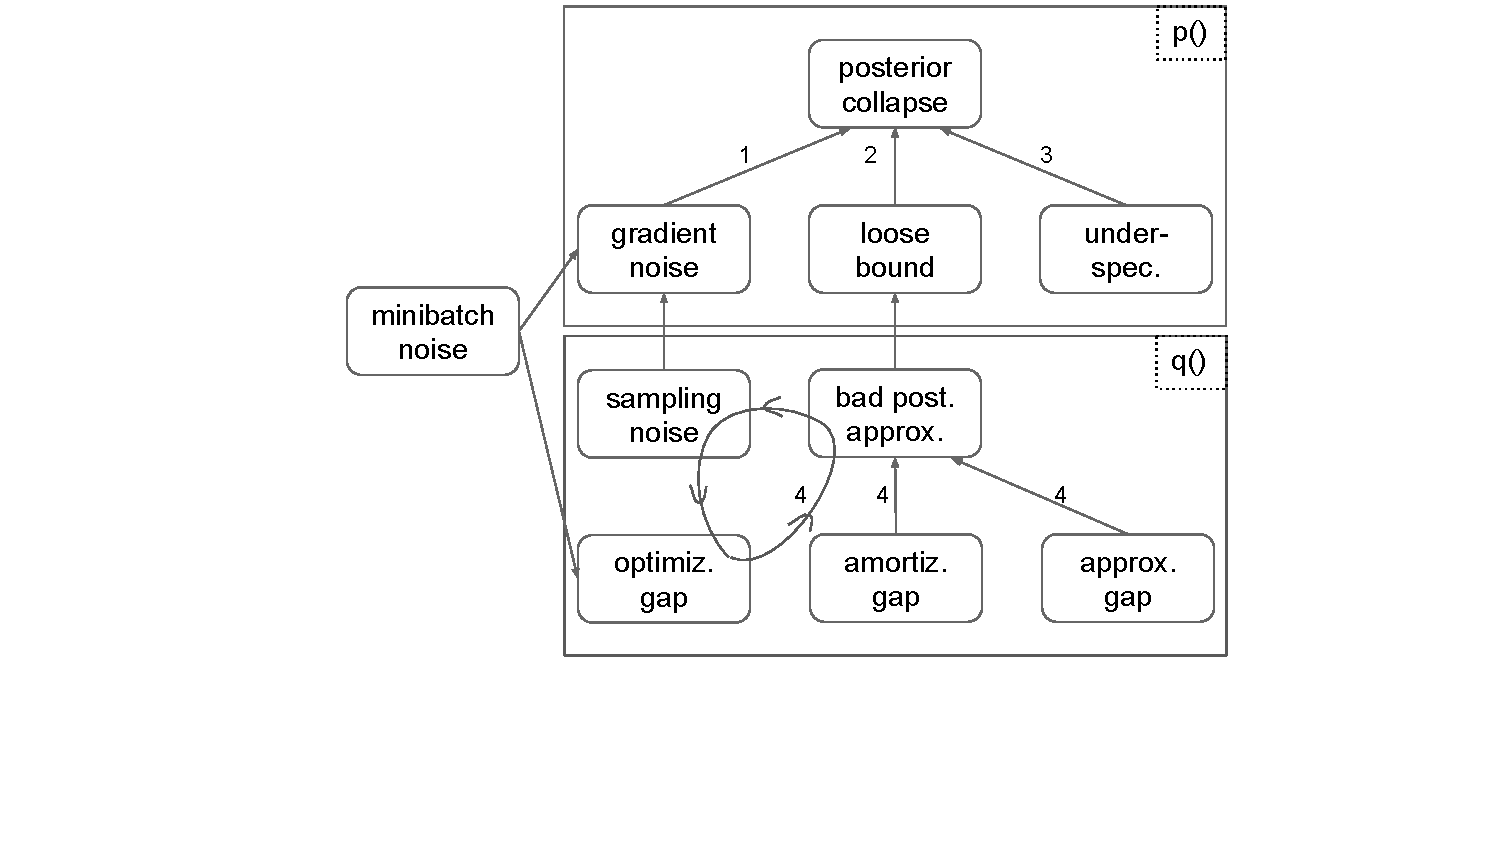
\includegraphics[scale=0.55,trim={4.5cm 3.2cm 2.5cm
        0.0cm},clip]{micmco/figure/posterior-collapse.pdf}
    \captionof{figure}[Causes of posterior collapse in VAEs.]{
      Causes of posterior collapse in VAEs. 1.~High variance gradient
      estimates and SGD's preference for flat minima exerts pressure
      to reduce variance by ignoring the latents. 2.~A loose lower
      bound underestimates the benefits of the latents.
      3.~Underspecification can allow posterior collapse to be the
      theoretical optimum. 4.~Posterior collapse reduces or eliminates
      all of the gaps and the sampling noise.}
    \label{fig:posterior-collapse}
  \end{minipage}
\end{figure}

The issues in what we observe as posterior collapse (or its milder form, the underuse of latents) span a number of causes.
\Cref{fig:posterior-collapse} summarizes the main known contributors to posterior collapse and their interactions.
At a glance, the immediate causes are high-variance gradient estimates, a loose lower bound, and underspecification.
\begin{itemize}
\item \textbf{Gradient noise}:
Optimization can be adversely affected by high-variance gradient estimators \citep{roeder2017sticking,tucker2018doubly} and minibatch noise in stochastic gradient descent \citep{titsias2014doubly}.
Unlike minibatch noise, sampling noise --~the variance induced by the latents~-- can be eliminated by ignoring the latents.
Because the looseness of the lower bound is proportional to the sampling variance \citep{maddison2017filtering}, coupled with SGD's preference for flat minima \citep{hochreiter1995simplifying}, this biases optimization towards posterior collapse.
\item \textbf{Loose lower bound}:
As its posterior-contrastive form \eqref{eq:elbo-posterior-contrastive} suggests, the ELBO is tight if $q(z\tmid x)$ matches $p(z\tmid x)$, and the worse the approximation, the looser the ELBO.
However, perfect posterior approximation might be hard or impossible to achieve, depending on the following factors \citep{cremer2017reinterpreting}.
\begin{itemize}
\item[\textbf{-}] The \textbf{approximation gap} is the distance of the true posterior from the variational family $\mathcal{Q}$ if $p(z\tmid x) \not\in \mathcal{Q}$ \citep{DBLP:conf/nips/ShuBZKE18,razavi2018preventing}.
\item[\textbf{-}] The \textbf{amortization gap} is the gap caused by the encoder's inability to represent the optimal $q_{\phi^\star}(z\tmid x)$ (which is $p_\theta(z\tmid x)$) for all $x$ with the same $\phi$ \citep{kim2018semi,DBLP:conf/nips/ShuBZKE18}.
\item[\textbf{-}] The \textbf{optimization gap} is caused the suboptimality of $q_\phi(z\tmid x)$ found by the optimizer relative to $q_{\phi^\star}(z\tmid x)$ \citep{he2018lagging}.
\end{itemize}
Notably, there is a negative feedback loop: optimization difficulties cause bad posterior approximation, which increases the variance induced by sampling the latents, which makes optimization harder.
\item \textbf{Underspecification}: As argued by \citet{alemi2017fixing}, the ELBO is neutral with respect to the mutual information, and even perfect optimization can land anywhere on the rate-distortion curve (the expected likelihood of the data as a function of the mutual information of the data and the latents).
More generally, the optimization task for generative models of the form $p(x,z)= p(x\tmid z)p(z)$ is often underspecified \citep{huszar2017representation}, which we explore in \Cref{sec:cia-an-pc}.
\end{itemize}

Unfortunately, posterior collapse reduces or eliminates all of the gaps and also the sampling noise, which makes the bound tight.
For VAEs to use their latent variables reliably and optimally, all of the above issues must be addressed.
The direction we take here delegates the problem of dealing with the looseness of the bound to a Monte Carlo estimator of the marginal likelihood, such as IWAE, and that of reducing gradient noise to a corresponding gradient estimator, such as DReG or VIMCO.
Importantly, in addition to providing tighter bounds, Monte Carlo estimators employ multiple samples from $q(z\tmid x)$, which benefits our efforts to tackle the issue of underspecification by designing better estimators of the mutual information.

\section{Related Works}

With several interacting issues to disentangle, the body of work on posterior collapse has grown large and disparate.
Many works aim to make the prior or the posterior more flexible to tighten the lower bound \citep{rezende2015variational,kingma2016improved,tomczak2018vae}.
At the same time, \citet{DBLP:conf/nips/ShuBZKE18} argue that while it is tempting to think that the variational family $\mathcal{Q}$ and $q_{\phi}(z\tmid x)$ should be as large and as flexible possible, a more restrictive choice can prove useful in performing posterior regularization.
\Citet{kim2018semi} propose reducing the amortization gap by only initializing the value of the latent variables according to the encoder, then optimizing their values separately for each example as in non-amortized variational inference \citep{jordan1999introduction}.
\Citet{he2018lagging} focus on improving the approximation quality of $q_\phi(z\tmid x)$ by taking several optimization steps on $\phi$ for each update of $\theta$ in $p_{\theta}$.
\Citet{yang2017improved} replace an auto-regressive decoder with dilated convolutions to restrict the available context and to thus enforce the use of the latents.
\Citet{van2017neural} introduce categorically distributed latents with a fixed KL cost and replace the prior with the aggregate posterior, which eliminates any pressure to ignore the latents.

Instead of completely eliminating the pressure to ignore the latents, controlling the KL term in \eqref{eq:elbo-prior-contrastive} by reducing its cost also received lots of attention.
Downweighting or annealing it during training is common \citep{bowman2015generating,higgins2016beta,sonderby2016ladder,NEURIPS2019_9bdb8b1f,NEURIPS2018_65b0df23}.
\Citet{kingma2016improved} flat spot the KL term so that small KL values are not penalized.
\Citet{razavi2018preventing} achieve a similar effect by choosing the variational family and the approximate posterior such that there is always an approximation gap.

Several works \citep{alemi2017fixing,zhao2019infovae,mccarthy2019improved,rezaabad2020learning,serdega2020vmi} recognize the issue of underspecification and propose to constrain the mutual information.
All work with single sample VAEs and the representational KL.
In contrast, we propose combining multi-sample Monte Carlo objectives with  estimates based on the true KL.
As we will see, this results in our mutual information estimates being less tied to the quality of $q(z\tmid x)$, while containing the single-sample, representational KL scenario as a degenerate case.

\section{CIA and Posterior Collapse}
\label{sec:cia-an-pc}

In this section, we explore \emph{why} our models are underspecified to better understand whether constraining the mutual information is a good solution.
More specifically, we ask under what conditional independence assumptions (CIA\footnote{Due to CIA being a collective noun in other contexts, we let its singular form stand also for its plural.}) can posterior collapse be an optimal solution for \emph{any} model to abstract away from finite capacities and optimization difficulties.
The next proposition shows that the answer is in fact trivial: the independence assumptions can be satisfied with a model where the latent and the observable variables are independent and the model matches the data distribution perfectly if and only if the independence assumptions are compatible with the marginal distribution of the data.

In particular, we consider Bayesian networks, given as 
\begin{align*}
p(x,z)=p(z) \prod_{i=1}^n p\condp[\big]{x_i}{\mathrm{pa}(i),\indcia},
\end{align*}
where $\mathrm{pa}(i)$ denotes the set of parent nodes of $x_i$, i.e.\ those on which it directly depends, and the first $k$ $x_i$ directly depend also on $z$.

\begin{proposition}
Let $\{x_i\}$, $i \in [1,n]$, be a partitioning of $x$, and $\mathrm{pa}(i) \subseteq \{x_i\}$.
For any prior $p(z)$, there exists a distribution\footnote{Here we consider the set of all distributions and not only the parameterized family $\{p_\theta\}$.}
$p(x,z)$ satisfying, for all $x$ and $z$,
\begin{enumerate}[(i)]
\item $p(x,z)=p(x)p(z)$ \hspace{0.1em} (posterior collapse);
\item $p(x)=p_D(x)$ \hspace{0.1em} (perfectly modelling the data);
\item $p(x,z)= p(z) \prod_{i=1}^n p\condp[\big]{x_i}{\mathrm{pa}(i),\indcia}$ for some $k \leqslant n$ \hspace{0.1em} (CIA)
\end{enumerate}
if and only if $p_D(x)=\prod_{i=1}^n p_D(x_i\tmid \mathrm{pa}(i))$ \hspace{0.1em} (the data distribution is compatible with the CIA of (iii)).
\end{proposition}
\begin{proof}
If $p_D(x)=\prod_{i=1}^n p_D(x_i\tmid \mathrm{pa}(i))$, then it is easy to check that $p(x,z)=p_D(x)\allowbreak{}p(z)$ satisfies the conditions (i)--(iii) with $k=0$.
To prove the other direction, assume (i)--(iii) hold.
Then (i) and (iii) imply that $p(x)=\prod_{i=1}^n p\condp[\big]{x_i}{\mathrm{pa}(i),\indcia}$ for all $z$.
Also, from (i) it follows that $\bigl(\textrm{pa}(i), x_i\bigr) \indep z$, and hence for all $z$, $p\condp{x_i}{\mathrm{pa}(i),z} = p\condp{x_i,\mathrm{pa}(i)}{z}/p\condp{\mathrm{pa}(i)}{z}=p(x_i\tmid \mathrm{pa}(i))$, giving $p(x)=\prod_{i=1}^n p(x_i\tmid \mathrm{pa}(i))$.
Finally, from (ii) we have that the two joints, $p_D(x)$ and $p(x)$ are the same, therefore their marginals and conditionals are the same too, which implies $p_D(x) = \prod_{i=1}^n\allowbreak p_D(x_i\tmid \mathrm{pa}(i))$.
\end{proof}

The proposition says that just by specifying CIA for otherwise dependent parts of the data, any model that suffers posterior collapse (in the sense that $x$ and $z$ are independent) will be suboptimal in terms of the model evidence $p(x)$.
This gives a degree of assurance that given such a structure, a well-optimized model with high enough capacity will not suffer posterior collapse.
Latent variable image models, which model pixels or patches conditionally independently given the latents fall into this category, which explains while posterior collapse is not so prevalent in that case.

Conversely, in theory and in the absence of CIA, there is a trivial latent variable model $p(x,z)=p_D(x)p(z)$ that is optimal in terms of the marginal likelihood $p(x)$ but does not use the latents.
The prototypical example for this case is auto-regressive likelihoods, such as RNN language models.

To summarize, \emph{CIA must be made} to guarantee that latents are used given powerful enough models and inference methods.
On the other hand, lacking the necessary CIA, we can still bias solutions by changing the objective.
One such change to compensate for the lack of model structure is adding a constraint on mutual information.

\section{Mutual Information Augmented Objectives}
\label{sec:mi-objective}

Mutual information is often used as a measure of latent variable usage in trained models or as part of the training objective to control latent usage and reduce underspecification.
First, as a measure of latent usage, it is a diagnostic of the inference method.
In this role, it is but a proxy for the generalization ability of the model or for the performance on down-stream tasks.
Second, as a constraint during training, it can be seen as compensating for the lack of structure in the model.
However, its role is not essential in either of these: evaluating representations without the down-stream tasks is fraught with peril, and equipping the model with structure sounds a rather more appealing direction to pursue.
Still, finding a good model structure is easier said than done, and in practice mutual information is useful both as a diagnostic for inference and as a tool for model specification.
Thus, we augment the marginal likelihood objective with a mutual information term and maximize
\begin{align}
\label{eq:mi-obj}
\E_{p_D(x)}\ln p(x) + \lambda I_p(X,Z),
\end{align}
where $p_D(x)$ is the data distribution and $\lambda \in \Rb, \lambda
\geqslant 0$.
Throughout, we assume that $I_p(X,Z)$ is bounded, which is satisfied by any model for which the optimization of $p(x)$ is well-posed and hence its $p(x\tmid z)$ is bounded for all $z$.
Also note that for any given $I_p(X,Z)$, the model achieves its global maximum when $p(x)=p_D(x)$, and we can reasonably expect models that suffer from posterior collapse to effectively balance data fit and mutual information.

Motivated by the identity $I_p(X,Z)=\E_{p(x)} \KL\Div{p(z\tmid x)}{p(z)}$, the mutual information term can be estimated by the average KL divergence.
While this true KL is hard to compute in general due to the intractable posterior, the availability of the variational posterior offers the compelling alternative of estimating $I_p(X,Z)$ with
\begin{align*}
I^{q,p}_{p_D}(X,Z) \coloneqq \E_{p_D(x)} \KL\Div[\big]{q(z\tmid x)}{p(z)}.
\end{align*}
Note the shortcut of sampling from $p_D(x)$ instead of $p(x)$.
If we plan to use the representations obtained from the variational posterior $q(z\tmid x)$ on some task, then $I^{q,p}_{p_D}$ is a natural quantity to track \citep{zhao2019infovae,rezaabad2020learning}.
However, in this work, our primary concern lies not with artifacts of variational inference but with the model $p(x,z)$ and its ability to capture information in the latents.
Moreover, employing $I^{q,p}_{p_D}$ as a proxy objective is problematic because it overestimates $I_p$ as $q$ tends to underestimate the variance of the true posterior.\footnote{For VAEs, this follows from the properties of the KL divergence, while for Monte Carlo objectives in general, it follows from how the looseness of the lower bound relates to the variance of the estimator \citep{maddison2017filtering}.}
Even worse, with $I^{q,p}_{p_D}$ the quality of $q(z\tmid x)$ would influence our conclusions about latent variable usage.
Monte Carlo objectives, whose $q(z\tmid x)$ in itself is no longer a direct approximation to $p(z\tmid x)$ \citep{mnih2016variational}, exacerbate the problem with latent usage estimation.
Experimentally, we found that, for models trained with Monte Carlo objectives, $I^{q,p}_{p_D}$ can wildly under- or overestimate $I_p$.
Thus, to form a better estimate of $I_p$, we replace $q(z\tmid x)$ with $p(z\tmid x)$ in $I^{q,p}_{p_D}$:
\begin{align}
\label{eq:cross-mi}
I_{p_D}^p(X,Z) \coloneqq \E_{p_D(x)} \KL\Div[\big]{p(z\tmid x)}{p(z)}.
\end{align}
This `cross' mutual information $I_{p_D}^p$ is the average true KL over the data distribution $p_D$.
Averaging over $p_D(x)$ instead of $p(x)$ is common practice as it allows the mutual information to be estimated based on the current minibatch without sampling from the model in the typical doubly stochastic optimization setting \citep{titsias2014doubly}.
The price for efficiency is a possible generalization problem: the average KL may be different over $p_D(x)$ and $p(x)$.
Generalization may eventually become a pressing issue, but as our experiments in \Cref{sec:micmco-experiments} will demonstrate, we first have to deal with underfitting.
In addition to being expedient, as we will show in \Cref{sec:connection-to-the-representational-kl} and \Cref{sec:connection-to-the-beta-vae}, this choice makes the single-sample case of our estimators correspond to the representational KL and the \betavae{} \citep{higgins2016beta}.

%%\mgl{Show that $\lambda>0$ implies maximial latent usage?}

\begin{definition}[Mutual information augmented objective]
The mutual information augmented objective, which is a  combination of the usual marginal likelihood objective and $I_{p_D}^p$, is defined as
\begin{align}
\label{eq:cross-mi-obj}
\mathcal{O}(\lambda) = \E_{p_D(x)} \ln p(x) + \lambda I_{p_D}^p(X,Z).
\end{align}
Furthermore, the pointwise version of the objective is defined as
\begin{equation}
\label{eq:cross-mi-obj-x}
\mathcal{O}(\lambda,x) = \ln p(x) + \lambda \KL\Div[\big]{p(z\tmid x)}{p(z)},
\end{equation}
which in turn satisfies $\mathcal{O}(\lambda) = \E_{p_D(x)} \mathcal{O}(\lambda,x)$.
\end{definition}

In the following, we propose estimators of $\mathcal{O}(\lambda,x)$ and the true KL within it to estimate $\mathcal{O}(\lambda)$ and the mutual information in a manner suitable for the doubly stochastic optimization setting.

\subsection{The KL Objective}

To find the maximum of $\mathcal{O}(\lambda)$ in $\theta$, both of its terms must be estimated well.
We delegate the task of estimating the marginal log-likelihood $\ln p(x)$ to a `base' Monte Carlo estimator of the form $\hat{S}^K(x,z_{1:K}) = \ln\left( \tfrac{1}{K} \sum_{i=1}^K f(x, z_i)\right)$, where $z_{1:K}=(z_1, \ldots, z_K)$ are independent samples from the proposal distribution $q(z\tmid x)$, and $f$ is some function of the observable and latent variables \citep{mnih2016variational}.
Ideally, $\hat{S}^K$ is chosen to have low bias and low variance, allowing optimization to strike a better balance with mutual information.
For our first contribution, the KL objective, we rewrite the true KL in a form more amenable to importance sampling:
\begin{align*}
\KL\Div[\big]{p(z\tmid x)}{p(z)}
&= \E_{p(z\tmid x)} \ln \frac{p(z\tmid x)}{p(z)}\\
&= \E_{p(z\tmid x)} \bigl[ \ln p(x\tmid z) \bigr] - \ln p(x)
\end{align*}
\begin{align*}
&= \E_{q(z\tmid x)} \biggl[ \frac{p(z\tmid x)}{q(z\tmid x)} \ln p(x\tmid z) \biggr] - \ln p(x)\\
&= \frac{1}{p(x)} \E_{q(z\tmid x)} \biggl[ \frac{p(x,z)}{q(z\tmid x)} \ln p(x\tmid z) \biggr]
   - \ln p(x).
\end{align*}
Plugging this into the definition of $\mathcal{O}(\lambda,x)$ in \eqref{eq:cross-mi-obj-x} and grouping the $\ln p(x)$ terms, we get
\begin{align*}
\mathcal{O}(\lambda,x)
%% &= \ln p(x) + \lambda \KL\Div[\big]{p(z\tmid x)}{p(z)} \\
%% &= \ln p(x) +
%%    \lambda \biggl( \frac{1}{p(x)} \E_{q(z\tmid x)} \biggl[ \frac{p(x,z)}{q(z\tmid x)}
%%                                                    \ln p(x\tmid z) \biggr]
%%                   - \ln p(x) \biggr) \\
&= (1-\lambda)\ln p(x) +
   \lambda \frac{1}{p(x)} \E_{q(z\tmid x)} \frac{p(x,z)}{q(z\tmid x)} \ln p(x\tmid z).
\end{align*}
In this form of the mutual information augmented objective, the first term, $(1-\lambda)\ln p(x)$, can be estimated with the base Monte Carlo estimator $\hat{S}^K$, so we only have the task of dealing the second term
\begin{align*}
\numberthis\label{eq:kl-plus-is}
\frac{1}{p(x)} \E_{q(z\tmid x)} \frac{p(x,z)}{q(z\tmid x)} \ln p(x\tmid z).
\end{align*}
Here, $p(x)$ could be estimated with the simple $K$-sample importance sampling estimator
\begin{align}
\label{eq:p-hat-k}
\hat{p}^K(x, z_{1:K}) \coloneqq \frac{1}{K} \sum_{i=1}^K \frac{p(x,z_i)}{q(z_i\tmid x)}.
\end{align}
However, combining $\hat{p}^K$ with an importance sampling estimate of the expectation in \eqref{eq:kl-plus-is} using different samples begot very high variance in preliminary experiments.
Instead, we approximate \eqref{eq:kl-plus-is} with the self-normalized importance sampling estimator
\begin{align*}
%\KL\Div[\big]{p(z\tmid x)}{p(z)} + \ln p(x)
%&= \frac{1}{p(x)} \E_{q(z\tmid x)} \frac{p(x,z)}{q(z\tmid x)} \ln p(x\tmid z) \\
\numberthis\label{eq:kl-estimator}
%&\approx
\hat{U}^K(x,z_{1:K})
 \coloneqq \hat{p}^K(x, z_{1:K})^{-1}
           \frac{1}{K} \sum_{i=1}^K \frac{p(x,z_i)}{q(z_i\tmid x)} \ln p(x\tmid z_i),
\end{align*}
which uses the same samples for estimating $1/p(x)$ and the expectation.
This leads to our first estimator for $\mathcal{O}(\lambda,x)$.

\begin{definition}[KL objective]
Let $\hat{S}^K$ be any $K$-sample Monte Carlo estimator of $\ln p(x)$.
Then the augmented objective $\mathcal{O}(\lambda,x)$ can be estimated by
the KL objective
\begin{align}
\label{eq:kl-obj}
\mathcal{O}_{\KL}(\hat{S}, K, \lambda,x)
&= \E_{z_{1:K}\sim q(z\tmid x)} \hat{O}_{\KL}(\hat{S}, K, \lambda, x, z_{1:K}),\\
\intertext{where}
\label{eq:kl-obj-estimator}
\mathcal{\hat{O}}_{\KL}(\hat{S}, K, \lambda, x, z_{1:K})
&= (1-\lambda)\hat{S}^K(x,z_{1:K}) + \lambda \hat{U}^K(x,z_{1:K}).
\end{align}
\end{definition}

Note that $\mathcal{\hat{O}}_{\KL}(\hat{S}^K, K, \lambda, x, z_{1:K})$ uses the same samples $z_{1:K} \sim q(z\tmid x)$ to estimate both terms of the augmented objective \eqref{eq:cross-mi-obj-x}.
Grouping the terms differently, we can separate out the estimate of the KL:
\begin{align}
\label{eq:kl-obj-estimator-alt}
\mathcal{\hat{O}}_{\KL}(\hat{S}, K, \lambda, x, z_{1:K})
&= \underbrace{\hat{S}^K(x,z_{1:K})}_{\approx \ln p(x)} +
   \lambda \underbrace{\bigl( \hat{U}^K(x,z_{1:K}) - \hat{S}^K(x,z_{1:K}) \bigr)}_{\approx \KL\Div{p(z\tmid x)}{p(z)}}.
\end{align}
We assume throughout that the estimators $\hat{S}^K(x,z_{1:K})$ and $\hat{U}^K(x,z_{1:K})$ have finite variance.
The estimators $\mathcal{\hat{O}}_{\KL}(\hat{S}^K, K, \lambda, x)$ of $\mathcal{O}(\lambda, x)$ and $\hat{U}^K(x,z_{1:K}) - \hat{S}^K(x,z_{1:K})$ of $\KL\Div{p(z\tmid x)}{p(z)}$ have the following properties:

\begin{proposition}[properties of the KL objective]
\label{prop:properties of the KL objective} \mbox{}
\begin{enumerate}[(i)]
\item If $\hat{S}^K$ converges in probability or almost surely to $\ln p(x)$ as $K \to \infty$, then so do $\mathcal{\hat{O}}_{\KL}$ and $\hat{U}^K - \hat{S}^K$ to
$\mathcal{O}(\lambda, x)$ and $\KL\Div{p(z\tmid x)}{p(z)}$, respectively.
\item If $\E_{z_{1:K} \sim q(z\tmid x)}\hat{S}^K(x,z_{1:K}) \leqslant \ln p(x)$, then
\begin{equation*}
\E_{z_{1:K} \sim q(z\tmid x)}[\hat{U}^K(x,z_{1:K}) - \hat{S}^K(x,z_{1:K})] \geqslant \KL\Div{p(z\tmid x)}{p(z)}.
\end{equation*}
That is, the estimator is biased upward.
\item The bias of the self-normalized importance sampling estimator $\hat{U}^K$ is bounded if $p(x,z)$ is bounded as shown in Proposition 7 of \citet{metelli2020importance}.
\item The variance of $\hat{U}^K$ decays with $K$, but unlike in non-normalized importance sampling, for any given $K$, there is no proposal distribution with which the variance is zero unless $\hat{U}^K$ is constant for all $z_{1:K}$ with probability 1.
\end{enumerate}
\end{proposition}
\begin{proof}
These follow from  the properties of self-normalized importance sampling \citep{art2013mcbook} except where noted.
\end{proof}

Note that although the objective is biased upwards, its bias is decreased with more samples and is bounded if $p(x,z)$ is bounded.
It can be assumed that $p(x,z)$ is bounded, else the optimization of $\ln p(x)$ is ill-posed even without the mutual information term.
Consequently we may be able to rely on $\lambda$ to counteract the bias thus bounded.
Importantly, the computation of $\hat{U}^K$ imposes minimal overhead as it needs to evaluate only $p(x\tmid z_i)$, $p(z_i)$ and $q(z_i\tmid x)$: the same quantities and same $z_i$ as needed for computing $\hat{S}^K$.
Referring back to \eqref{eq:mi-obj}, we argue that this KL objective allows for effective interpolation between fitting the data and capturing information in the latent variables.

\subsection{The Rényi Objective}
\label{sec:renyi-objective}

In this section, we introduce a second estimator of the augmented objective $\mathcal{O}(\lambda, x)$ \eqref{eq:cross-mi-obj-x}, based on the Rényi divergence, to address a potential issue with the KL objective's estimate \eqref{eq:kl-obj-estimator}.
This issue lies in the fact that the KL objective linearly combines two estimators ($\hat{S}^K$ and $\hat{U}^K$) of different quantities.
How their biases and variances relate deserves some consideration.
As we have seen, with $\hat{S}^K$ that underestimate $\ln p(x)$ (e.g.\ IWAE), $\hat{U}^K-\hat{S}^K$ overestimates the true KL.
Luckily, both biases can be reduced with more samples.

However, taking more samples may not help if the two estimators have very different variances, in which case optimizing the objective may be difficult.
This issue could be addressed by designing a $\hat{U}^K$ for every $\hat{S}^K$, but this would limit the applicability of our method in practice.
Instead, we apply $\hat{S}$ not only to estimate $\ln p(x)$ but \emph{a second time} too to estimate the Rényi divergence, itself a biased estimate of the true KL.
As we will see later, this works surprisingly well in practice despite the presence of the bias.

The Rényi divergence between two distributions $f(x)$ and $g(x)$ is defined as $D_\alpha\Div{f}{g}=\frac{1}{\alpha-1}\ln \E_{g(x)} f(x)^\alpha g(x)^{-\alpha}$, where $\alpha$ is a positive real number.
For $\alpha<1$, $D_\alpha\Div{f}{g} \leqslant \KL\Div{f}{g}$, while for $\alpha>1$, $D_\alpha\Div{f}{g} \geqslant \KL\Div{f}{g}$.
Since $\lim_{\alpha \to 1} D_\alpha\Div{f}{g} = \KL\Div{f}{g})$,  $D_\alpha\Div{f}{g}$ can approximate $\KL\Div{f}{g}$ arbitrarily closely when $\alpha$ is sufficiently close to $1$.
This latter property motivates the use of $D_\alpha\Div{p(z\tmid x)}{p(z)}$ as an approximation to the true KL.
To construct an estimator, we first rewrite the Rényi divergence as:
\begin{align*}
(\alpha-1)D_\alpha\Div[\big]{p(z\tmid x)}{p(z)}
&= \ln \E_{p(z)} \frac{p(z\tmid x)^\alpha}{p(z)^\alpha}\\
&= \ln \E_{p(z)} \biggl[ \frac{p(z\tmid x)^\alpha p(x)^\alpha}{p(z)^\alpha} \biggr]
   - \alpha \ln p(x)\\
&= \ln \E_{p(z)} \bigl[ p(x\tmid z)^\alpha \bigr] - \alpha \ln p(x)\\
\numberthis\label{eq:renyi-rewrite}
&= \ln p^\alpha(x) - \alpha \ln p(x),
\end{align*}
where $p^\alpha(x)\coloneqq\E_{p(z)} p(x\tmid z)^\alpha$.

We note in passing that $p^\alpha(x)$ has an intuitive interpretation, particularly when $\alpha \in \Nb$.
Consider the task of modelling the distribution of discrete data over some discrete set $\cX$ duplicated $\alpha$ times, that is $p^\alpha_D(x, \ldots, x) \coloneqq p_D(x)$.
That is, $p^\alpha_D$ is a probability distribution over $\cX^\alpha$, whereas $p_D$ is over $\cX$, and $p^\alpha_D(x_1, \ldots, x_\alpha)=0$ unless all $x_i$ are identical.
On this task, $\alpha \ln p(x) = \ln p(x)^\alpha$ acts as the uninformed baseline, in which a separate set of latents is used for each branch $p(x_i\tmid z)$, thus the cost of information in the latents must be paid $\alpha$ times.
This means that, based on its alternative form $\ln p^\alpha(x) - \alpha \ln p(x)$ in \eqref{eq:renyi-rewrite}, we can interpret the Rényi divergence as a measure of how much better the $\alpha$-duplicated model $p^\alpha(x)$ does at modelling the duplicated data compared to the worst-case solution $p(x)^\alpha$, which does not use the latents to amortize the cost of encoding the data multiple times.

\noindent We now derive a biased approximation to $\mathcal{O}(\lambda,x)$:
\begin{align*}
\mathcal{O}(\lambda,x)
&= \ln p(x) + \lambda \KL\Div[\big]{p(z\tmid x)}{p(z)}\\
&\approx \ln p(x) + \lambda D_\alpha\Div[\big]{p(z\tmid x)}{p(z)}\\
&= \ln p(x) + \frac{\lambda}{\alpha-1} \bigl(\ln p^\alpha(x) - \alpha \ln p(x)\bigr)\\
&= \frac{\lambda}{\alpha-1} \ln p^\alpha(x)
   - \biggl(\frac{\lambda\alpha}{\alpha-1}-1\biggr) \ln p(x).
\end{align*}

\begin{definition}[Rényi objective]
Let $\lambda, \alpha>0$, and let $\hat{S}^K(x,z_{1:K})$ and $\hat{S}^K_\alpha(x,z_{1:K})$ be $K$-sample Monte Carlo estimators for $\ln p(x)$ and $\ln p^\alpha(x)$, respectively.
Then the augmented objective $\mathcal{O}(\lambda,x)$ can be estimated by
the Rényi objective
\begin{align}
\label{eq:renyi-obj}
\mathcal{O}_{R}(\hat{S}, K, \lambda, \alpha, x)
&= \E_{z_{1:K}\sim q(z\tmid x)} \mathcal{\hat{O}}_{R}(\hat{S}, K, \lambda, \alpha, x, z_{1:K}),
\intertext{where}
\label{eq:renyi-obj-estimator}
\mathcal{\hat{O}}_{R}(\hat{S}, K, \lambda, \alpha, x, z_{1:K})
&= \frac{\lambda}{\alpha-1} \hat{S}^K_\alpha(x,z_{1:K})
   - \biggl(\frac{\lambda\alpha}{\alpha-1}-1\biggr) \hat{S}^K(x,z_{1:K}).
\end{align}
\end{definition}

\noindent Separating out the estimate of the Rényi divergence yields the alternative form
\begin{align}
\label{eq:renyi-obj-estimator-alt}
\mathcal{\hat{O}}_{R}(\hat{S}, K, \lambda, \alpha, x, z_{1:K})
&= \underbrace{\hat{S}^K(x, z_{1:K})}_{\approx \ln p(x)}
   + \lambda \underbrace{ \biggl( \frac{1}{\alpha-1}
                                 \Bigl( \hat{S}^K_\alpha(x,z_{1:K}) -
                                       \alpha \hat{S}^K(x,z_{1:K}) \Bigr)
                          \biggr)
                        }_{\approx D_\alpha\Div{p(z\tmid x)}{p(z)}}.
\end{align}

Our goal was to address the mismatched biases and variances of the KL objective's $\hat{S}^K$ and $\hat{U}^K$.
Having eliminated $\hat{U}^K$, we are left with only $\hat{S}^K$ and $\hat{S}^K_\alpha$, estimating two closely related quantities, $\ln p(x)$ and $\ln p^\alpha(x)$.
Note that $\hat{S}^K_\alpha$ can be obtained with a slight modification of $\hat{S}^K$, as explained in the next section.
In \Cref{sec:micmco-experiments}, we validate experimentally that the benefits this scheme affords outweigh the obvious drawback of additional bias in the Rényi objective.

\subsubsection{Estimating \texorpdfstring{$p^\alpha(x)$}{palpha(x)} with IWAE}

From $\ln p(x) = \ln\left(\E_{p(z)} p(x\tmid z)\right)$ and $\ln p^\alpha(x) = \ln \left(\E_{p(z)} p(x\tmid z)^\alpha\right)$, we have that if $\hat{S}^K(x,z_{1:K})$ is computed explicitly in terms of $p(x\tmid z)$, then $\hat{S}^K_\alpha(x,z_{1:K})$ can be derived simply by replacing $p(x\tmid z)$ with $p(x\tmid z)^\alpha$ in $\hat{S}^K(x, z_{1:K})$.
All base estimators considered here have this property and we elucidate the derivation through the example of the IWAE.

The ELBO of variational autoencoders can be rather loose, and the variance of the resulting approximate posterior is usually smaller than that of the true posterior.
To tackle these issues, \cite{burda2015importance} proposed the importance weighted autoencoder (IWAE).
Whereas the ELBO is single-sample, the IWAE bound is based on $K \in \Nb$ samples:
\begin{align*}
\ln p(x)
= \ln \E_{p(z)} p(x\tmid z)
&= \ln \E_{\substack{z_1,\ldots, z_K\\ \sim q(z\tmid x)}}
  \frac{1}{K} \sum_{i=1}^K \frac{p(x\tmid z_i)p(z_i)}{q(z_i\tmid x)}\\
&\geqslant \E_{\substack{z_1,\ldots, z_K\\ \sim q(z\tmid x)}}
  \ln \frac{1}{K} \sum_{i=1}^K \frac{p(x\tmid z_i)p(z_i)}{q(z_i\tmid x)}.
\end{align*}

In importance sampling terms, $p(x\tmid z)$ is the integrand, the function whose expectation we want to compute with respect to $p(z)$.
While $p(x\tmid z)$ here is a probability mass function, importance sampling does not require this.
In fact, we can estimate the expectation of $p(x\tmid z)^\alpha$ analogously:
\begin{align*}
\numberthis
\label{eq:power-iwae-bound}
\ln p^\alpha(x)
%% = \ln \E_{p(z)} p(x\tmid z)^\alpha
%% &= \ln \E_{\substack{z_1,\ldots, z_K\\ \sim q(z\tmid x)}}
%%   \frac{1}{K} \sum_{i=1}^K \frac{p(x\tmid z_i)^\alpha p(z)}{q(z_i\tmid x)}\\
&\geqslant \E_{\substack{z_1,\ldots, z_K\\ \sim q(z\tmid x)}}
  \ln \frac{1}{K} \sum_{i=1}^K \frac{p(x\tmid z_i)^\alpha p(z_i)}{q(z_i\tmid x)}.
\end{align*}
To estimate the expectation in the above lower bound, we can recombine $p(x\tmid z_i)$, $p(z_i)$ and $q(z_i\tmid x)$, quantities already computed for the base estimator, with negligible computational overhead.

Note that there is an optimal proposal distribution  $q_{\text{opt}}(z\tmid x)=p(x\tmid z)^\alpha p(z) /\allowbreak p^\alpha(x)$ that leads to exactly computing $\ln p^\alpha(x)$ (i.e.\ estimating it with zero bias and variance).
On the other hand, the other term in the Rényi objective is best estimated using, in general, a different proposal distribution.
One solution would be to apply separate proposal distributions, another is to choose $\lambda$ and $\alpha$ such that in $\ln p(x) + \lambda D_\alpha$ the $\ln p(x)$ term is cancelled out, which we explore briefly in \Cref{sec:power-objective} below.

\subsubsection{Other Estimators}

In the interest of space, we omit re-derivations of further estimators of $\ln p^\alpha(x)$ and their gradient estimators.
As in the IWAE case, all we need to show is that the estimators do not depend on properties of $p(x\tmid z)$ that $p^\alpha(x\tmid z)$ does not have, and for performance, that $p(x\tmid z)$ is explicitly computed so that computing $p(x\tmid z)^\alpha$ is cheap.
These are true for the estimators used in our experiments: REINFORCE \citep{williams1987class,mnih2014neural}, VIMCO \citep{mnih2016variational}, STL \citep{roeder2017sticking} and DReG \citep{tucker2018doubly}.

\subsection{The Power Objective}
\label{sec:power-objective}

Notice that, in the Rényi estimator \eqref{eq:renyi-obj-estimator}, if $\lambda$ is set to $(\alpha-1)/\alpha$, then the coefficient of the $\ln p(x)$ term becomes zero, yielding a simpler form.

\begin{definition}[Power objective]
We call the Rényi objective with $\lambda=(\alpha-1)/\alpha$ the \emph{power objective}:
\begin{align*}
\numberthis\label{eq:power-obj}
%% \mathcal{O} \approx
\mathcal{\hat{O}}_P(\hat{S}, K, \alpha, x, z_{1:K})
= \alpha^{-1} \hat{S}^K_\alpha(x,z_{1:K}).
\end{align*}
\end{definition}

Note that for optimization the constant $\alpha^{-1}$ can be dropped from the objective and that if $\alpha=1$, the power objective is equal to the log-likelihood $\ln p(x)$.
Next we show that if $\alpha>1$, maximizing $p^\alpha(x)$ optimizes a lower bound on $p(x)$, and this lower bound is tight when the latents fully determine the observables.
\begin{restatable}{proposition}{proppowerlowerbound}
\label{prop:power-lower-bound}
Assume that $X$ is concentrated on the countable set $\cX$, $\alpha>1$, and let $x \in \cX$ be arbitrary. Then $p^\alpha(x) \leqslant p(x)$ with equality for all $x \in \cX$ if and only if $H_p(X\tmid Z)=0$.
Second, $p(x)^\alpha \leqslant p^\alpha(x)$ and $\ln p^\alpha(x) - \alpha \ln p(x) = (\alpha-1)D_\alpha\Div{p(z\tmid x)}{p(z)}$.
\end{restatable}
\begin{proof}
Since $X$ is countable, $p(x\tmid z)$ is discrete, hence $p(x\tmid z) \leqslant 1$ for all $x$ and $z$. Therefore, since $\alpha>1$, $p(x\tmid z)^\alpha \leqslant p(x\tmid z)$ with equality if and only if $p(x\tmid z) \in \{0,1\}$. Thus,
$p^\alpha(x)
= \E_{p(z)} p(x\tmid z)^\alpha \leqslant \E_{p(z)} p(x\tmid z)
= p(x)$,
with equality if and only if $p(x\tmid z) \in \{0,1\}$ for all $x$, for almost all $z$. The latter holds if and only if $X$ is a deterministic function of $Z$ with probability 1, which is equivalent to $H_p(X\tmid Z)=0$.
The second statement of is a direct consequence of \eqref{eq:renyi-rewrite} and both $\alpha-1$ and the Rényi divergence being non-negative.
\end{proof}

So the power objective with $\alpha>1$ is an upper bound on the KL (and $I_{p_D}^p$ when averaged over $x$), but this upper bound nevertheless becomes tight when the latents determine the observable variables (i.e.\ when $H_p(X\tmid Z)=0$).

In summary, the power objective has three important differences from the Rényi objective, of which it is a special case.
First, with $\alpha>1$, it is guaranteed to be a lower bound on $\ln p(x)$.
Second, since there is only a single quantity, $\ln p^\alpha(x)$, being estimated, the question of using separate $q(z\tmid x)$ proposal distributions to estimate the different terms does not arise.
Third, $\lambda$ and $\alpha$ are tied, so it may be harder to find a good balance between ease of optimization and low bias.
Whether the power objective's benefits outweigh its downsides is investigated in \Cref{sec:micmco-experiments-with-the-power-objective}.

\section{Connection to the Representational KL}
\label{sec:connection-to-the-representational-kl}

\begin{proposition}[Single-sample KL estimate]
\label{prop:single-sample-kl-estimate}
In the single-sample case with $\hat{S}^1(x, z_1) = \ln \frac{p(x,z_1)}{q(z_1\tmid x)}$, the KL objective's estimate of the true KL in \eqref{eq:kl-obj-estimator-alt} is the representational KL in expectation:
\begin{align*}
\E_{z_1 \sim q(z\tmid x)} \bigl[ \hat{U}^1(x,z_1) - \hat{S}^1(x,z_1) \bigr] = \KL\Div[\big]{q(z\tmid x)}{p(z)}.
\end{align*}
\end{proposition}
\begin{proof}
With $\hat{p}^1(x, z_1) = p(x,z_1)/q(z_1\tmid x)$ from \eqref{eq:p-hat-k}, we have that
\begin{align*}
\hat{U}^1(x,&z_1) - \hat{S}^1(x,z_1)\\
&= \hat{p}^1(x, z_1)^{-1} \frac{p(x,z_1)}{q(z_1\tmid x)} \ln p(x\tmid z_1) -
   \ln \frac{p(x,z_1)}{q(z_1\tmid x)} \\
&= \ln p(x\tmid z_1) - \ln \frac{p(x,z_1)}{q(z_1\tmid x)}
= \ln \frac{q(z_1\tmid x)}{p(z_1)}.
\qedhere
\end{align*}
\end{proof}

So not only are the expectations the same, but our single-sample estimate is the same as the trivial single-sample estimate of the representational KL.
We now prove a similar result for the Rényi objective.

\begin{proposition}[Single-sample Rényi estimate]
\label{prop:single-sample-renyi-estimate}
In the single-sample case with $\hat{S}^1(x, z_1)\allowbreak{}= \ln \frac{p(x,z_1)}{q(z_1\tmid x)}$, the Rényi objective's estimate of $D_\alpha{p(z\tmid x)}{p(z)}$ in \eqref{eq:renyi-obj-estimator-alt} is the representational KL in expectation:
{\def\groundprop{4}
\begin{align*}
\E_{z_1 \sim q(z\tmid x)} \biggl[ \frac{1}{\alpha-1}
                                 \Bigl( \hat{S}^1_\alpha(x,z_1) -
                                       \alpha \hat{S}^1(x,z_1) \Bigr)
                 \biggr]
= \KL\Div[\big]{q(z\tmid x)}{p(z)}.
\end{align*}}%
\end{proposition}
\begin{proof}
Let us rewrite the expression in the expectation.
\begin{align*}
\frac{1}{\alpha-1} \biggl( &\hat{S}^1_\alpha(x,z_1) - \alpha \hat{S}^1(x,z_1) \biggr)\\
&= \frac{1}{\alpha-1}\biggl(\ln \frac{p(x\tmid z_1)^\alpha p(z_1)}{q(z_1\tmid x)} - \alpha \ln \frac{p(x,z_1)}{q(z_1\tmid x)}\biggr)\\
&= \frac{1}{\alpha-1}\biggl(\ln \frac{p(z_1)}{q(z_1\tmid x)} - \alpha \ln \frac{p(z_1)}{q(z_1\tmid x)}\biggr)\\
&= \ln \frac{q(z_1\tmid x)}{p(z_1)}
\qedhere
\end{align*}
\end{proof}

In the single-sample case, where $q(z\tmid x)$ approximates the true posterior much better compared to the multi-sample Monte Carlo estimators, the representational KL approximates the true KL with a relatively small bias.
This bias is, however, asymptotically eliminated by our KL estimator as the number of samples $K$ grows (and reduced for our Rényi estimator), which significantly improves the usage of the latent variables.
This is demonstrated in our experiments (e.g.\ \Cref{fig:synthetic-dreg-samples,fig:synthetic-vimco-samples}) where we compare methods using KL estimates based on different number of samples from $q(z\tmid x)$.

\section[Connection to the $\upbeta$-VAE]{Connection to the \texorpdfstring{{\protect\scriptsizerrr$\upbeta$}}{Beta}-VAE}
\label{sec:connection-to-the-beta-vae}

In parallel to the single-sample case of our estimators, we now show that the \betavae{} \citep{higgins2016beta} objective defined as
{\def\groundprop{1.5}
\begin{align}
\label{eq:beta-vae-obj}
\mathcal{O}_{\beta\text{-VAE}}(\beta, x)
= \E_{z_1 \sim q(z\tmid x)} \bigl[ \ln p(x\tmid z_1) \bigr] - \beta \KL\Div[\big]{q(z\tmid x)}{p(z)}
\end{align}}%
is equal to the KL, Rényi and power objectives with suitably chosen parameters.

\begin{proposition}[\betavae{} equivalence]
In the single-sample case with $\hat{S}^1(x, z_1) = \ln \frac{p(x,z_1)}{q(z_1\tmid x)}$, the \betavae{} and our single-sample objectives are equal with a suitable choice of $\lambda$ or $\alpha$:
{\setlength{\jot}{0.5\groundskip}
\begin{align*}
\mathcal{O}_{\beta\text{-VAE}}(\beta, x)
&= \mathcal{O}_{\KL}(\hat{S}, 1, 1-\beta, x)
 & \qquad \text{($\lambda=1-\beta$)}\\
&= \mathcal{O}_R(\hat{S}, 1, 1-\beta, \alpha, x)
 & \qquad \text{($\lambda=1-\beta$)}\\
&= \mathcal{O}_P(\hat{S}, 1, \beta^{-1}, x)
 & \qquad \text{($\alpha=\beta^{-1}$)}.
\end{align*}}%
\end{proposition}
\begin{proof}
We prove the KL objective case from \eqref{eq:kl-obj-estimator-alt} and \Cref{prop:single-sample-kl-estimate}:
\begin{align*}
\E_{z_1 \sim q(z\tmid x)} & \mathcal{\hat{O}}_{\KL}(\hat{S}, 1, \lambda, x, z_1)\\
&= \E_{z_1 \sim q(z\tmid x)} \bigl[ \hat{S}^1(x,z_1) \bigr] +
   \lambda \E_{z_1 \sim q(z\tmid x)} \bigl[ \hat{U}^1(x,z_1) - \hat{S}^1(x,z_1) \bigr]\\
&= \E_{z_1 \sim q(z\tmid x)} \biggl[ \ln \frac{p(x,z_1)}{q(z_1\tmid x)} \biggr]
    + \lambda \KL\Div[\big]{q(z\tmid x)}{p(z)}\\
&= \E_{z_1 \sim q(z\tmid x)} \bigl[ \ln p(x\tmid z_1) \bigr]
   + (\lambda - 1) \KL\Div[\big]{q(z\tmid x)}{p(z)}.
\end{align*}
The proof for the Rényi case follows a similar route, starting from \eqref{eq:renyi-obj-estimator-alt} and using \Cref{prop:single-sample-renyi-estimate}.
Finally, for the power objective, $\lambda = (\alpha-1)/\alpha$, so $\alpha=\beta^{-1}$ recovers $\lambda = 1-\beta$.
\end{proof}

\section{Experiments}
\label{sec:micmco-experiments}

The goal of our experiments is to demonstrate the difficulty of inference with VAEs and Monte Carlo objectives and to evaluate the proposed methods.
Our results indicate the presence of a severe tradeoff between data fit and latent variable usage.
We emphasize that, for progress to be made, the choice of evaluation method must acknowledge the existence of this tradeoff.
In this work, evaluation is performed in terms of Pareto frontiers of data likelihood vs latent usage curves; reporting a single, best data likelihood would always pick the point with zero latent usage.
Results with our proposed estimators, either with continuous latents and DReG or discrete latents and the VIMCO base estimator, markedly improve on their baselines, which do not have multiple samples or cannot use them as efficiently.
The improvement is especially significant with discrete latents.

Instead of trying to improve the predictive performance directly, first we demonstrate the difficulty of inference on a simple, synthetic data set and a model to which posterior collapse comes easy.
These experiments focus exclusively on data fit to highlight the tradeoff against latent usage.
After the experiments on synthetic data, we move on to language modelling with recurrent networks, a very hostile application for VAEs \citep{bowman2015generating}.

\subsection{Experiments with Synthetic Data}
\label{sec:micmco-experiments-with-synthetic-data}

Every data point is a single symbol drawn from a discrete uniform distribution over a vocabulary of 10000 symbols.
The optimal solution is to assign probability 1/10000 to each symbol, which can be trivially satisfied by a simple model that ignores the latents.
Note that $\lambda>0$ makes such solutions suboptimal.
In fact, for all priors such that $H(Z)\geqslant H(X)$, the optimal solution must capture all information in the latents (i.e.\ $I(X,Z)=H(X)$).
Our goal with these experiments is to demonstrate the difficulty of fitting the data while using the latents.

\subsubsection{Model Architecture}

The encoder implementing $q$ assigns an embedding \citep{mikolov2013distributed} to each word in the vocabulary, feeds the embedding to a two-layer, densely connected neural network with $\tanh$ non-linearities.
For continuous latents, $q(z\tmid x)$ follows an isotropic normal distribution $\N(f(o),\diag(\exp(g(o))))$, where $f$ and $g$ are affine transformations parameterized as densely connected layers, and $o$ is the output of the last encoder layer for a given $x$.
For categorical latents, $q(z\tmid x)$ is proportional to $\exp(o)$ (i.e.\ it is a categorical distribution parameterized with $\softmax(o)$).
The decoder is similar to the encoder but with a final softmax layer.
In the decoder, values of continuous latents are fed directly as input to the first layer, but values of categorical latents are first embedded.
To compensate for this discrepancy, decoders with categorical latents have only one hidden layer.
All embeddings and hidden layers are of size 128.

\subsubsection{Evaluation Methodology}

Since there is no single number to summarize the tradeoff between latent usage and the quality of the model, we plot the model's latent usage and the expected negative log-likelihood (NLL).
The NLL of optimal solutions is the entropy of the data distribution, $\ln 10000\approx 9.210$.
The models' NLLs are estimated using IWAE with 100 samples.
We quantify latent variable usage as the mutual information $I_p(X,Z)$, estimated as the average $\hat{U}^K(x, z_{1:K}) - \ln \hat{p}^K(x, z_{1:K})$ \eqref{eq:kl-estimator} with $K=100$ samples.
We validated empirically that the variance of these estimates is small ($<0.01$) over all feasible latent usage values.
Zero latent usage corresponds to posterior collapse.

These plots (like Figure 3b in \citealt{alemi2017fixing}) carry the same information as rate-distortion curves, which can be recovered by subtracting the rate $I_p$ from the NLL.
Only the measurements on the Pareto frontier are shown, and we tune hyperparemeters, such as the learning rate and $\lambda$, of the augmented objective \eqref{eq:cross-mi-obj} to push the Pareto frontier towards more efficient latent usage.
See \Cref{sec:optimization-settings} for details.

\subsubsection{Overview of Results}

Results for continuous and discrete latents are presented in separate sections, following a similar progression:
\begin{itemize}
\item We first show that the choice of base estimator matters: the variance issues of IWAE and REINFORCE limit the potential of the proposed method.
\item Next, with DReG and VIMCO we present clear improvements over the single-sample baselines.
\item Finally, as an ablation study, we verify that using multiple samples in both the marginal likelihood and the mutual information terms of the objective is necessary for best performance.
\end{itemize}
We also note that without augmenting the objective with a mutual information term, our model tends to fit the data perfectly with negligible latent usage.
These degenerate curves consisting of a single point are omitted from the plots.

% {fig:synthetic-iwae}
\begin{figure}
\begin{tikzpicture}
\begin{axis}[xmin=-0.01,xmax=9.22,ymin=9.20,ymax=9.45,
  xlabel=average KL, ylabel=Training NLL,
  height=0.33*\textwidth,
  width=0.98\textwidth,
  grid=major,
  legend pos=north west,
  legend columns=2,
  legend style={
    font=\mystrut,
    legend cell align=left,
    at={(0.18,0.98)},
    anchor=north west,
  },
]

\addlegendimage{legend image with text=KL}
\addlegendentry{}
\addlegendimage{legend image with text=Rényi}
\addlegendentry{}

\pgfplotstablesort[sort key=validklp]{\sorted}
                  {micmco/data/synthetic/l40x0-bs256-hs128-t40-vae-kl}
\addplot[redhollow] table [x=validklp, y=validnll] {\sorted};
\addlegendentry{};

\pgfplotstablesort[sort key=validklp]{\sorted}
                  {micmco/data/synthetic/l40x0-bs256-hs128-t40-vae-renyi}
\addplot[redsolid] table [x=validklp, y=validnll] {\sorted};
\addlegendentry{ELBO};

\pgfplotstablesort[sort key=validklp]{\sorted}
                  {micmco/data/synthetic/l40x0-bs256-hs128-t40-iwae1-kl}
\addplot[violethollow] table [x=validklp, y=validnll] {\sorted};
\addlegendentry{};

\pgfplotstablesort[sort key=validklp]{\sorted}
                  {micmco/data/synthetic/l40x0-bs256-hs128-t40-iwae1-renyi}
\addplot[violetsolid] table [x=validklp, y=validnll] {\sorted};
\addlegendentry{IWAE 1};

\pgfplotstablesort[sort key=validklp]{\sorted}
                  {micmco/data/synthetic/l40x0-bs256-hs128-t40-iwae16-kl};
\addplot[bluehollow] table [x=validklp, y=validnll] {\sorted};
\addlegendentry{};

\pgfplotstablesort[sort key=validklp]{\sorted}
                  {micmco/data/synthetic/l40x0-bs256-hs128-t40-iwae16-renyi}
\addplot[bluesolid] table [x=validklp, y=validnll] {\sorted};
\addlegendentry{IWAE 16};

\pgfplotstablesort[sort key=validklp]{\sorted}
                  {micmco/data/synthetic/l40x0-bs256-hs128-t40-iwae64-kl};
\addplot[tealhollow] table [x=validklp, y=validnll] {\sorted};
\addlegendentry{};

\pgfplotstablesort[sort key=validklp]{\sorted}
                  {micmco/data/synthetic/l40x0-bs256-hs128-t40-iwae64-renyi};
\addplot[tealsolid] table [x=validklp, y=validnll] {\sorted};
\addlegendentry{IWAE 64};

\end{axis}
\end{tikzpicture}
\caption[KL and Rényi objectives on continuous synthetic data with base estimators ELBO and IWAE.]{KL and Rényi objectives (empty and full markers) on continuous synthetic data with base estimators ELBO and IWAE N, where N is the number of samples used for estimating both $p(x)$ and $\KL\Div{p(z\tmid x)}{p(z)}$.
Here and in the following plots, without augmenting the objective with the mutual information term, models tend to fit the data perfectly with negligible latent usage.
These degenerate curves consisting of a single point are omitted from the plots.
Also, with base estimators ELBO and IWAE 1, our estimators are equivalent to a \betavae{} with analytical and estimated KL (see \Cref{sec:connection-to-the-beta-vae}), respectively.}
\label{fig:synthetic-iwae}
\end{figure}

% {fig:synthetic-dreg}
\begin{figure}
\begin{tikzpicture}
\begin{axis}[xmin=-0.01,xmax=9.22,ymin=9.20,ymax=9.45,
  xlabel=average KL, ylabel=Training NLL,
  height=0.33*\textwidth,
  width=0.98\textwidth,
  grid=major,
  legend pos=north west,
  legend columns=2,
  legend style={
    font=\mystrut,
    legend cell align=left,
    at={(0.18,0.98)},
    anchor=north west,
  },
]

\addlegendimage{legend image with text=KL}
\addlegendentry{}
\addlegendimage{legend image with text=Rényi}
\addlegendentry{}

\pgfplotstablesort[sort key=validklp]{\sorted}
                  {micmco/data/synthetic/l40x0-bs256-hs128-t40-vae-kl}
\addplot[redhollow] table [x=validklp, y=validnll] {\sorted};
\addlegendentry{};

\pgfplotstablesort[sort key=validklp]{\sorted}
                  {micmco/data/synthetic/l40x0-bs256-hs128-t40-vae-renyi}
\addplot[redsolid] table [x=validklp, y=validnll] {\sorted};
\addlegendentry{ELBO};

\pgfplotstablesort[sort key=validklp]{\sorted}
                  {micmco/data/synthetic/l40x0-bs256-hs128-t40-dreg1-kl}
\addplot[violethollow] table [x=validklp, y=validnll] {\sorted};
\addlegendentry{};

\pgfplotstablesort[sort key=validklp]{\sorted}
                  {micmco/data/synthetic/l40x0-bs256-hs128-t40-dreg1-renyi}
\addplot[violetsolid] table [x=validklp, y=validnll] {\sorted};
\addlegendentry{DReG 1};

\pgfplotstablesort[sort key=validklp]{\sorted}
                  {micmco/data/synthetic/l40x0-bs256-hs128-t40-dreg16-kl};
\addplot[bluehollow] table [x=validklp, y=validnll] {\sorted};
\addlegendentry{};

\pgfplotstablesort[sort key=validklp]{\sorted}
                  {micmco/data/synthetic/l40x0-bs256-hs128-t40-dreg16-renyi}
\addplot[bluesolid] table [x=validklp, y=validnll] {\sorted};
\addlegendentry{DReG 16};

\pgfplotstablesort[sort key=validklp]{\sorted}
                  {micmco/data/synthetic/l40x0-bs256-hs128-t40-dreg64-kl};
\addplot[tealhollow] table [x=validklp, y=validnll] {\sorted};
\addlegendentry{};

\pgfplotstablesort[sort key=validklp]{\sorted}
                  {micmco/data/synthetic/l40x0-bs256-hs128-t40-dreg64-renyi};
\addplot[tealsolid] table [x=validklp, y=validnll] {\sorted};
\addlegendentry{DReG 64};

\end{axis}
\end{tikzpicture}
\caption{KL and Rényi objectives on continuous synthetic data with base estimators ELBO, DReG.}
\label{fig:synthetic-dreg}
\end{figure}

\subsubsection{Continuous Latents}
With 40 continuous latents and an isotropic standard normal prior, the base estimator is either the standard ELBO, IWAE or IWAE-DReG.
In the ELBO, the KL term \eqref{eq:elbo-prior-contrastive} is computed analytically, while in IWAE 1, the single sample from the latents is used to estimate it.
An improvement to IWAE 1 is the STL estimator from \citet{roeder2017sticking}, which removes a zero-expectation term from the objective and whose gradients have zero variance when the variational approximation is exact.
IWAE--DReG, whose objective is also identical to that of IWAE, is a generalization of STL to multiple samples, fixing the signal-to-noise problem of gradient estimates of IWAE \citep{rainforth2018tighter}, wherein the magnitude of the gradient decreases faster with more samples than the variance of the gradient estimates.
Although DReG can also be applied to Reweighted Wake-Sleep \citep{bornschein2014reweighted} and Jackknife Variational Inference \citep{nowozin2018debiasing}, we only use IWAE--DReG in our experiments and let DReG stand for IWAE--DReG without ambiguity.

Our results in \Cref{fig:synthetic-iwae,fig:synthetic-dreg} are in agreement with these previous works.
In the context of this work, our findings can be summarized as follows.
\begin{itemize}
\item Compared to the theoretical optimum, a horizontal line at $\ln 10000 \approx 9.210$, all Pareto curves slope increasingly upwards with more latent usage.
\item Higher-variance estimators have steeper curves than lower variance estimators, which is most apparent in the contrast between two of our baselines, IWAE 1 and DReG 1.
\item The single sample estimators ELBO, IWAE 1, DReG 1 --~which are equivalent to a \betavae{} (\Cref{sec:connection-to-the-beta-vae})~-- are less efficient in their latent usage than our proposed multi-sample estimators.
\item The Rényi objective performs slightly better than the KL objective with the same base estimator.
\end{itemize}

In more detail, \Cref{fig:synthetic-iwae} shows that both of our estimators perform much worse with IWAE 1 as the base estimator than with the ELBO.
As the number of samples grows, this is reversed, although with a high number of samples we do see the predicted degradation \citep{rainforth2018tighter}.

Next, \Cref{fig:synthetic-dreg} confirms DReG's advantage over the IWAE, performing more efficiently than the ELBO even with a single sample.
Our multi-sample objectives both improve on the stronger baseline DReG 1 represents.
The Rényi objective outperforms the KL objective by a small but consistent margin before all estimators start degenerating quickly nearing the maximal average KL possible.

In \Cref{fig:synthetic-dreg-samples}, we take a closer look at the best performing DReG 16 base estimator to determine whether the improvements are due to a better estimate of the marginal likelihood $\ln p(x)$, or the mutual information term $I_{p_D}^p(X,Z)$ in \eqref{eq:cross-mi-obj}.
DReG 16/1 and DReG 1/16 (which use multiple samples to estimate only the marginal likelihood or the mutual information, respectively) are less efficient than DReG 16, sometimes being outperformed even by DReG 1.
Out of the two, DReG 1/16 performs better, indicating that the variance of the base estimator DReG 1 is low and the problem lies with the mutual information estimate.
These results support not only our observations in \Cref{sec:mi-objective} on the unsuitability of $I^{q,p}_{p_D}$ as an estimate of $I_p$ in the multi-sample case (DReG 16/1), when $q(z\tmid x)$ is not a good approximation of $p(z\tmid x)$, but also demonstrate that $I^{q,p}_{p_D}$ can be improved by taking multiple samples even when $\ln p(x)$ is estimated with a single sample and $q(z\tmid x)$ better approximates the true posterior $p(z\tmid x)$.

\begin{figure}
\begin{tikzpicture}
\begin{axis}[xmin=-0.01,xmax=9.22,ymin=9.20,ymax=9.45,
  xlabel=average KL, ylabel=Training NLL,
  height=0.33*\textwidth,
  width=0.98\textwidth,
  grid=major,
  legend pos=north west,
  legend columns=2,
  legend style={
    font=\mystrut,
    legend cell align=left,
    at={(0.18,0.98)},
    anchor=north west,
  },
]

\addlegendimage{legend image with text=KL}
\addlegendentry{}
\addlegendimage{legend image with text=Rényi}
\addlegendentry{}

\pgfplotstablesort[sort key=validklp]{\sorted}
                  {micmco/data/synthetic/l40x0-bs256-hs128-t40-dreg1-kl}
\addplot[redhollow] table [x=validklp, y=validnll] {\sorted};
\addlegendentry{};

\pgfplotstablesort[sort key=validklp]{\sorted}
                  {micmco/data/synthetic/l40x0-bs256-hs128-t40-dreg1-renyi}
\addplot[redsolid] table [x=validklp, y=validnll] {\sorted};
\addlegendentry{DReG 1};

\pgfplotstablesort[sort key=validklp]{\sorted}
                  {micmco/data/synthetic/l40x0-bs256-hs128-t40-dreg16-kl1};
\addplot[violethollow] table [x=validklp, y=validnll] {\sorted};
\addlegendentry{};

\pgfplotstablesort[sort key=validklp]{\sorted}
                  {micmco/data/synthetic/l40x0-bs256-hs128-t40-dreg16-renyi1}
\addplot[violetsolid] table [x=validklp, y=validnll] {\sorted};
\addlegendentry{DReG 16/1};

\pgfplotstablesort[sort key=validklp]{\sorted}
                  {micmco/data/synthetic/l40x0-bs256-hs128-t40-dreg1-kl16};
\addplot[bluehollow] table [x=validklp, y=validnll] {\sorted};
\addlegendentry{};

\pgfplotstablesort[sort key=validklp]{\sorted}
                  {micmco/data/synthetic/l40x0-bs256-hs128-t40-dreg1-renyi16}
\addplot[bluesolid] table [x=validklp, y=validnll] {\sorted};
\addlegendentry{DReG 1/16};

\pgfplotstablesort[sort key=validklp]{\sorted}
                  {micmco/data/synthetic/l40x0-bs256-hs128-t40-dreg16-kl};
\addplot[tealhollow] table [x=validklp, y=validnll] {\sorted};
\addlegendentry{};

\pgfplotstablesort[sort key=validklp]{\sorted}
                  {micmco/data/synthetic/l40x0-bs256-hs128-t40-dreg16-renyi};
\addplot[tealsolid] table [x=validklp, y=validnll] {\sorted};
\addlegendentry{DReG 16};

\end{axis}
\end{tikzpicture}
\caption[KL and Rényi objectives on continuous synthetic data with base estimator DReG.]{KL and Rényi objectives on continuous synthetic data with base estimator DReG. DReG 1 uses a single sample to estimate both $p(x)$ and $\KL\Div{p(z\tmid x)}{p(z)}$. DReG 16/1 uses 16 samples to estimate $p(x)$ and 1 sample for the KL. DReG 1/16 uses 1 sample to estimate $p(x)$ and 16 samples for the KL. Finally, DReG 16 uses the same 16 samples for both terms.}
\label{fig:synthetic-dreg-samples}
\end{figure}

\subsubsection{Discrete Latents}

Next we performed experiments with 8 categorical latent variables, each with a uniform prior over 10 categories.
Using the high-variance REINFORCE base estimator (\Cref{fig:synthetic-reinforce}), we could only get a small improvement over the single-sample case with 16 samples and a similar degradation with 64.

\begin{figure}
\begin{tikzpicture}
\begin{axis}[xmin=-0.01,xmax=9.22,ymin=9.20,ymax=9.45,
  xlabel=average KL, ylabel=Training NLL,
  height=0.32*\textwidth,
  width=0.98\textwidth,
  grid=major,
  legend pos=north west,
  legend columns=2,
  legend style={
    font=\mystrut,
    legend cell align=left,
  },
]

\addlegendimage{legend image with text=KL}
\addlegendentry{}
\addlegendimage{legend image with text=Rényi}
\addlegendentry{}

\pgfplotstablesort[sort key=validklp]{\sorted}
                  {micmco/data/synthetic/l8x10-bs256-hs128-t40-vimco1-kl}
\addplot[redhollow] table [x=validklp, y=validnll] {\sorted};
\addlegendentry{};

\pgfplotstablesort[sort key=validklp]{\sorted}
                  {micmco/data/synthetic/l8x10-bs256-hs128-t40-vimco1-renyi}
\addplot[redsolid] table [x=validklp, y=validnll] {\sorted};
\addlegendentry{REINFORCE 1};

\pgfplotstablesort[sort key=validklp]{\sorted}
                  {micmco/data/synthetic/l8x10-bs256-hs128-t40-reinforce16-kl};
\addplot[bluehollow] table [x=validklp, y=validnll] {\sorted};
\addlegendentry{};

\pgfplotstablesort[sort key=validklp]{\sorted}
                  {micmco/data/synthetic/l8x10-bs256-hs128-t40-reinforce16-renyi}
\addplot[bluesolid] table [x=validklp, y=validnll] {\sorted};
\addlegendentry{REINFORCE 16};

\pgfplotstablesort[sort key=validklp]{\sorted}
                  {micmco/data/synthetic/l8x10-bs256-hs128-t40-reinforce64-kl};
\addplot[tealhollow] table [x=validklp, y=validnll] {\sorted};
\addlegendentry{};

\pgfplotstablesort[sort key=validklp]{\sorted}
                  {micmco/data/synthetic/l8x10-bs256-hs128-t40-reinforce64-renyi};
\addplot[tealsolid] table [x=validklp, y=validnll] {\sorted};
\addlegendentry{REINFORCE 64};

\end{axis}
\end{tikzpicture}
\caption{KL and Rényi objectives on discrete synthetic data with base estimator REINFORCE.}
\label{fig:synthetic-reinforce}
\end{figure}

However, with the much lower variance VIMCO estimator, we achieved almost perfect results (see \Cref{fig:synthetic-vimco}) with 16 samples.
For our purposes, it suffices to think of VIMCO as IWAE applied to discrete latents with lower variance gradients.
It may be surprising that these results are even better than with continuous latents, especially at near-maximal latent usage.
To intuit why, consider the minimum variance posterior achievable for a given level of average KL.
For discrete latents, a hard posterior (i.e.\ of zero variance) is possible depending on the number of latents and categories.
For continuous latents, the posterior can never be hard: the mutual information determines a lower bound on the average variance of the posterior.

Increasing the number of samples further to 64 made results much worse, indicating a potential issue with VIMCO, which may be similar to the signal-to-noise issue that DReG addresses, but this is beyond the scope of the present work.
Note that there is no single-sample VIMCO since its baseline for the contribution of a sample is computed as the average over the rest of the samples, which is undefined.
Assuming a zero baseline, we recover REINFORCE 1, which we use for comparison wherever VIMCO 1 would be needed.

\begin{figure}
\begin{tikzpicture}
\begin{axis}[xmin=-0.01,xmax=9.22,ymin=9.20,ymax=9.45,
  xlabel=average KL, ylabel=Training NLL,
  height=0.32*\textwidth,
  width=0.98\textwidth,
  grid=major,
  legend columns=2,
  legend style={
    font=\mystrut,
    at={(0.6,0.98)},
    anchor=north west,
    legend cell align=left,
  },
]

\addlegendimage{legend image with text=KL}
\addlegendentry{}
\addlegendimage{legend image with text=Rényi}
\addlegendentry{}

\pgfplotstablesort[sort key=validklp]{\sorted}
                  {micmco/data/synthetic/l8x10-bs256-hs128-t40-vimco1-kl}
\addplot[redhollow] table [x=validklp, y=validnll] {\sorted};
\addlegendentry{};

\pgfplotstablesort[sort key=validklp]{\sorted}
                  {micmco/data/synthetic/l8x10-bs256-hs128-t40-vimco1-renyi}
\addplot[redsolid] table [x=validklp, y=validnll] {\sorted};
\addlegendentry{REINFORCE 1};

\pgfplotstablesort[sort key=validklp]{\sorted}
                  {micmco/data/synthetic/l8x10-bs256-hs128-t40-vimco16-kl};
\addplot[bluehollow] table [x=validklp, y=validnll] {\sorted};
\addlegendentry{};

\pgfplotstablesort[sort key=validklp]{\sorted}
                  {micmco/data/synthetic/l8x10-bs256-hs128-t40-vimco16-renyi}
\addplot[bluesolid] table [x=validklp, y=validnll] {\sorted};
\addlegendentry{VIMCO 16};

\pgfplotstablesort[sort key=validklp]{\sorted}
                  {micmco/data/synthetic/l8x10-bs256-hs128-t40-vimco64-kl};
\addplot[tealhollow] table [x=validklp, y=validnll] {\sorted};
\addlegendentry{};

\pgfplotstablesort[sort key=validklp]{\sorted}
                  {micmco/data/synthetic/l8x10-bs256-hs128-t40-vimco64-renyi};
\addplot[tealsolid] table [x=validklp, y=validnll] {\sorted};
\addlegendentry{VIMCO 64};

\end{axis}
\end{tikzpicture}
\caption[KL and Rényi objectives on discrete synthetic data with base estimator VIMCO.]{KL and Rényi objectives on discrete synthetic data with base estimator VIMCO. The single-sample VIMCO is equivalent to REINFORCE.}
\label{fig:synthetic-vimco}
\end{figure}

Similarly to \Cref{fig:synthetic-dreg-samples} in the continuous case, in \Cref{fig:synthetic-vimco-samples}, we try to tease apart the contributions of using multiple samples for estimating the marginal likelihood and mutual information terms of \eqref{eq:cross-mi-obj}.
The results are much more pronounced here.
Both VIMCO 16/1 and VIMCO 1/16 improve significantly on REINFORCE 1 but only with the Rényi objective.
Still, both fall way short of VIMCO 16, which employs multiple samples for both terms.
Again, these results support not only our observations in \Cref{sec:mi-objective} on the unsuitability of $I^{q,p}_{p_D}$ as an estimate of $I_p$ in the multi-sample case (DReG 16/1), when $q(z\tmid x)$ is not a good approximation of $p(z\tmid x)$, but also demonstrate that $I^{q,p}_{p_D}$ can be improved by taking multiple samples even when $\ln p(x)$ is estimated with a single sample and $q(z\tmid x)$ better approximates the true posterior $p(z\tmid x)$.

\begin{figure}
\begin{tikzpicture}
\begin{axis}[xmin=-0.01,xmax=9.22,ymin=9.20,ymax=9.45,
  xlabel=average KL, ylabel=Training NLL,
  height=0.32*\textwidth,
  width=0.98\textwidth,
  grid=major,
  legend pos=north west,
  legend columns=2,
  legend style={
    font=\mystrut,
    legend cell align=left,
    at={(0.03,0.97)},
    anchor=north west,
  },
]

\addlegendimage{legend image with text=KL}
\addlegendentry{}
\addlegendimage{legend image with text=Rényi}
\addlegendentry{}

\pgfplotstablesort[sort key=validklp]{\sorted}
                  {micmco/data/synthetic/l8x10-bs256-hs128-t40-vimco1-kl}
\addplot[redhollow] table [x=validklp, y=validnll] {\sorted};
\addlegendentry{};

\pgfplotstablesort[sort key=validklp]{\sorted}
                  {micmco/data/synthetic/l8x10-bs256-hs128-t40-vimco1-renyi}
\addplot[redsolid] table [x=validklp, y=validnll] {\sorted};
\addlegendentry{REINFORCE 1};

\pgfplotstablesort[sort key=validklp]{\sorted}
                  {micmco/data/synthetic/l8x10-bs256-hs128-t40-vimco16-kl1};
\addplot[violethollow] table [x=validklp, y=validnll] {\sorted};
\addlegendentry{};

\pgfplotstablesort[sort key=validklp]{\sorted}
                  {micmco/data/synthetic/l8x10-bs256-hs128-t40-vimco16-renyi1}
\addplot[violetsolid] table [x=validklp, y=validnll] {\sorted};
\addlegendentry{VIMCO 16/1};

\pgfplotstablesort[sort key=validklp]{\sorted}
                  {micmco/data/synthetic/l8x10-bs256-hs128-t40-vimco1-kl16};
\addplot[bluehollow] table [x=validklp, y=validnll] {\sorted};
\addlegendentry{};

\pgfplotstablesort[sort key=validklp]{\sorted}
                  {micmco/data/synthetic/l8x10-bs256-hs128-t40-vimco1-renyi16}
\addplot[bluesolid] table [x=validklp, y=validnll] {\sorted};
\addlegendentry{VIMCO 1/16};

\pgfplotstablesort[sort key=validklp]{\sorted}
                  {micmco/data/synthetic/l8x10-bs256-hs128-t40-vimco16-kl};
\addplot[tealhollow] table [x=validklp, y=validnll] {\sorted};
\addlegendentry{};

\pgfplotstablesort[sort key=validklp]{\sorted}
                  {micmco/data/synthetic/l8x10-bs256-hs128-t40-vimco16-renyi};
\addplot[tealsolid] table [x=validklp, y=validnll] {\sorted};
\addlegendentry{VIMCO 16};

\end{axis}
\end{tikzpicture}
\caption[KL and Rényi objectives on discrete synthetic data with base estimator VIMCO.]{KL and Rényi objectives on discrete synthetic data with base estimator VIMCO. REINFORCE 1 (standing in for VIMCO 1) uses a single sample to estimate both $p(x)$ and $\KL\Div{p(z\tmid x)}{p(z)}$. VIMCO 16/1 uses 16 samples to estimate $p(x)$ and 1 samples for the KL. VIMCO 1/16 uses 1 sample to estimate $p(x)$ and 16 samples for the KL. Finally, VIMCO 16 uses the same 16 samples for both terms.}
\label{fig:synthetic-vimco-samples}
\end{figure}

In \Cref{sec:additional-experiments-on-synthetic-data}, we also present results for the VQ-VAE \citep{van2017neural} \emph{without} augmenting its objective with a mutual information term.
Since the KL cost in VQ-VAEs is determined by the latent space and is fixed during training, we tune the number of latent variables and the number of categories to control the mutual information.
Results of the VQ-VAE are better than REINFORCE but much worse than VIMCO 16 with either the KL or the Rényi objective.

\subsection{Language Modelling Experiments}
\label{sec:language-modelling-experiments}

One of the most challenging applications of variational autoencoders is language modelling with per-sentence latents, as found by \citet{bowman2015generating}.
They recognize the generality of the underspecification issue and attribute the increased difficulty to `the sensitivity of the LSTM to subtle variations in its hidden state as introduced by the sampling process'.
In this section, we first show that the data fit vs latent usage tradeoff is even more pronounced in the language modelling case than on the synthetic task, then confirm that the proposed estimators improve validation set results in terms of the Pareto frontiers.
Once again, the improvement is strongest with discrete latents.

\subsubsection{Data Set}

We do sentence-level language modelling on the Penn Treebank (PTB) corpus by \citet{marcus1993building} with preprocessing from \citet{mikolov2010recurrent}.
Our goal here is to compare inference methods, not to establish a new state of the art, so to reduce the computational burden brought about by hyperparemeter tuning, we truncated sentences to 35 tokens in both the training and validation sets, with a reduction of 3\% in the total number of tokens.
This truncation is non-standard.

\subsubsection{Model Architecture}

The model architecture is like in the synthetic case except the encoder embeds the input tokens and feeds them to a one-layer, bidirectional LSTM \citep{hochreiter1997long} and the output $o$ (from which the parameters of the variational posterior $q(z\tmid x)$ are computed) is the average of the last states of LSTMs corresponding to the two directions.
There is a fixed number of latents for all sentences, regardless of their length.
The decoder is a unidirectional LSTM whose input is the embedding of the previous token plus the values of the latent variables.
Unless stated otherwise, the embedding and hidden sizes are all 128.
Similarly to the synthetic case, we use either 40 real-valued latents with an isotropic standard normal prior or 8 categorical latent variables, each with a uniform prior over 10 categories.

\subsubsection{Evaluation Methodology}

Following previous works, both the reported NLL and the average KL values are averages over tokens in the data set.
Since there is only a single set of latents per sentence, this means that the average sentence-level KL is about 21 (the average number of tokens per sentence) times larger.
For expediency, only the base estimators that performed best on the synthetic data set are considered, leaving us with DReG for continuous, and VIMCO for discrete latents.
Training and validation NLLs are estimated using IWAE with 100 samples.
Test NLLs in \Cref{tab:ptb-best-nlls} are estimated using IWAE with 500 samples.

% {fig:ptb-dreg-train}
\begin{figure}
\begin{tikzpicture}
\begin{axis}[xmin=-0.01,xmax=2.01,ymin=2.21,ymax=3.3,ytick distance=0.2,
  xlabel=per-token KL, ylabel=Training NLL,
  height=0.32*\textwidth,
  width=0.98\textwidth,
  grid=major,
  legend pos=south east,
  legend columns=2,
  legend style={
    font=\mystrut,
    legend cell align=left,
  },
]

\addlegendimage{legend image with text=KL}
\addlegendentry{}
\addlegendimage{legend image with text=Rényi}
\addlegendentry{}

\pgfplotstablesort[sort key=validklp]{\sorted}
                  {micmco/data/l40x0-bs256-hs128-t40-dreg1-kl}
\addplot[redhollow] table [x=validklp, y=validnll] {\sorted};
\addlegendentry{};

\pgfplotstablesort[sort key=validklp]{\sorted}
                  {micmco/data/l40x0-bs256-hs128-t40-dreg1-renyi}
\addplot[redsolid] table [x=validklp, y=validnll] {\sorted};
\addlegendentry{DReG 1};

\pgfplotstablesort[sort key=validklp]{\sorted}
                  {micmco/data/l40x0-bs256-hs128-t40-dreg16-kl};
\addplot[bluehollow] table [x=validklp, y=validnll] {\sorted};
\addlegendentry{};

\pgfplotstablesort[sort key=validklp]{\sorted}
                  {micmco/data/l40x0-bs256-hs128-t40-dreg16-renyi}
\addplot[bluesolid] table [x=validklp, y=validnll] {\sorted};
\addlegendentry{DReG 16};

\pgfplotstablesort[sort key=validklp]{\sorted}
                  {micmco/data/l40x0-bs256-hs128-t40-dreg64-kl};
\addplot[tealhollow] table [x=validklp, y=validnll] {\sorted};
\addlegendentry{};

\pgfplotstablesort[sort key=validklp]{\sorted}
                  {micmco/data/l40x0-bs256-hs128-t40-dreg64-renyi};
\addplot[tealsolid] table [x=validklp, y=validnll] {\sorted};
\addlegendentry{DReG 64};

\end{axis}
\end{tikzpicture}
\caption[KL and Rényi objectives on Penn Treebank with base estimator DReG.]{KL and Rényi objectives (empty and full markers, respectively) on Penn Treebank with base estimators DReG N, where N is the number of samples used for estimating both $p(x)$ and $\KL\Div{p(z\tmid x)}{p(z)}$.}
\label{fig:ptb-dreg-train}
\end{figure}

% {fig:ptb-vimco-train}
\begin{figure}
\begin{tikzpicture}
\begin{axis}[xmin=-0.01,xmax=2.01,ymin=2.21,ymax=3.3,ytick distance=0.2,
  xlabel=per-token KL, ylabel=Training NLL,
  height=0.32*\textwidth,
  width=0.98\textwidth,
  grid=major,
  legend pos=south east,
  legend columns=2,
  legend style={
    font=\mystrut,
    legend cell align=left,
  },
]

\addlegendimage{legend image with text=KL}
\addlegendentry{}
\addlegendimage{legend image with text=Rényi}
\addlegendentry{}

\pgfplotstablesort[sort key=validklp]{\sorted}
                  {micmco/data/l8x10-bs256-hs128-t40-vimco1-kl}
\addplot[redhollow] table [x=validklp, y=validnll] {\sorted};
\addlegendentry{};

\pgfplotstablesort[sort key=validklp]{\sorted}
                  {micmco/data/l8x10-bs256-hs128-t40-vimco1-renyi}
\addplot[redsolid] table [x=validklp, y=validnll] {\sorted};
\addlegendentry{REINFORCE 1};

\pgfplotstablesort[sort key=validklp]{\sorted}
                  {micmco/data/l8x10-bs256-hs128-t40-vimco16-kl};
\addplot[bluehollow] table [x=validklp, y=validnll] {\sorted};
\addlegendentry{};

\pgfplotstablesort[sort key=validklp]{\sorted}
                  {micmco/data/l8x10-bs256-hs128-t40-vimco16-renyi}
\addplot[bluesolid] table [x=validklp, y=validnll] {\sorted};
\addlegendentry{VIMCO 16};

\pgfplotstablesort[sort key=validklp]{\sorted}
                  {micmco/data/l8x10-bs256-hs128-t40-vimco64-kl};
\addplot[tealhollow] table [x=validklp, y=validnll] {\sorted};
\addlegendentry{};

\pgfplotstablesort[sort key=validklp]{\sorted}
                  {micmco/data/l8x10-bs256-hs128-t40-vimco64-renyi};
\addplot[tealsolid] table [x=validklp, y=validnll] {\sorted};
\addlegendentry{VIMCO 64};

\end{axis}
\end{tikzpicture}
\caption{KL and Rényi objectives on PTB with base estimator VIMCO.}
\label{fig:ptb-vimco-train}
\end{figure}

\subsubsection{Training Fit}
In terms of training fit, the language modelling results are similar to those of the synthetic case.
In \Cref{fig:ptb-dreg-train}, there is improvement in the continuous case with multiple samples, initially with both the KL and the Rényi objectives but only with the Rényi at high latent usage.

\Cref{fig:ptb-vimco-train} shows the discrete latents case.
Once again, with either the KL or the Rényi objective, the results improve markedly, outperforming the continuous models.
Note that the KL range is limited by the entropy of the latent space at around $\ln(10^8) / 21 \approx 0.87$.
Furthermore, as \Cref{sec:additional-language-modelling-experiments-asymmetric-samples} shows, improvements in training fit require multiple samples in both terms, even more so than in the experiments on the synthetic data earlier.

% {fig:ptb-naive-dropout-valid}
\begin{figure}
\begin{tikzpicture}
\begin{axis}[xmin=-0.01,xmax=2.01,ymin=4.5,ymax=5.5,
  xlabel=per-token KL, ylabel=Validation NLL,
  height=0.33*\textwidth,
  width=0.98\textwidth,
  grid=major,
  legend pos=south east,
  legend columns=2,
  legend style={
    font=\mystrut,
    legend cell align=left,
  },
]

\addlegendimage{legend image with text=DReG}
\addlegendentry{}
\addlegendimage{legend image with text=VIMCO}
\addlegendentry{}

\pgfplotstablesort[sort key=validklp]{\sorted}
                  {micmco/data/l40x0-bs256-hs128-t40-dreg1-kl-valid}
\addplot[redhollow] table [x=validklp, y=validnll] {\sorted};
\addlegendentry{}

\pgfplotstablesort[sort key=validklp]{\sorted}
                  {micmco/data/l8x10-bs256-hs128-t40-vimco1-kl-valid}
\addplot[redsolid] table [x=validklp, y=validnll] {\sorted};
\addlegendentry{1 K}

\pgfplotstablesort[sort key=validklp]{\sorted}
                  {micmco/data/l8x10-bs256-hs128-t40-vimco16-kl-valid}
\addplot[bluehollow] table [x=validklp, y=validnll] {\sorted};
\addlegendentry{}

\pgfplotstablesort[sort key=validklp]{\sorted}
                  {micmco/data/l40x0-bs256-hs128-t40-dreg16-kl-valid}
\addplot[bluesolid] table [x=validklp, y=validnll] {\sorted};
\addlegendentry{16 K}

\pgfplotstablesort[sort key=validklp]{\sorted}
                  {micmco/data/l40x0-bs256-hs128-t40-dreg16-renyi-valid}
\addplot[tealhollow] table [x=validklp, y=validnll] {\sorted};
\addlegendentry{}

\pgfplotstablesort[sort key=validklp]{\sorted}
                  {micmco/data/l8x10-bs256-hs128-t40-vimco16-renyi-valid}
\addplot[tealsolid] table [x=validklp, y=validnll] {\sorted};
\addlegendentry{16 R}

\end{axis}
\end{tikzpicture}
\caption[Validation NLL with naive dropout using DReG and VIMCO on PTB.]{Validation NLL with naive dropout using DReG and VIMCO on PTB. The row with \emph{16 K} refers to 16-sample DReG or VIMCO with the KL objective, while \emph{R} stands for the Rényi objective.}
\label{fig:ptb-naive-dropout-valid}
\end{figure}

\subsubsection{Validation and Test Results}

Our initial results on the validation set were not very positive.
We tuned hyperparameters on the validation set, where following \cite{melis2017state}, we introduced three additional hyperparameters in the decoder: the rate of dropout applied to the input embedding, the recurrent state, and the output embedding.
As \Cref{fig:ptb-naive-dropout-valid} shows, with this strong form of regularization, the multi-sample results brought no improvement with continuous latents.
With discrete latents, the results improved but not nearly to the extent observed on the training set, and discrete latents performed considerably worse than their continuous counterparts.

% {fig:ptb-l2-penalty-valid}
\begin{figure}
\begin{tikzpicture}
\begin{axis}[xmin=-0.01,xmax=2.01,ymin=4.5,ymax=5.5,
  xlabel=per-token KL, ylabel=Validation NLL,
  height=0.33*\textwidth,
  width=0.98\textwidth,
  grid=major,
  legend pos=south east,
  legend columns=2,
  legend style={
    font=\mystrut,
    legend cell align=left,
  },
]

\addlegendimage{legend image with text=DReG}
\addlegendentry{}
\addlegendimage{legend image with text=VIMCO}
\addlegendentry{}

\pgfplotstablesort[sort key=validklp]{\sorted}
                  {micmco/data/l40x0-bs256-hs128-t40-dreg1-kl-valid-l2}
\addplot[redhollow] table [x=validklp, y=validnll] {\sorted};
\addlegendentry{}

\pgfplotstablesort[sort key=validklp]{\sorted}
                  {micmco/data/l8x10-bs256-hs128-t40-vimco1-kl-valid-l2}
\addplot[redsolid] table [x=validklp, y=validnll] {\sorted};
\addlegendentry{1 K}

\pgfplotstablesort[sort key=validklp]{\sorted}
                  {micmco/data/l40x0-bs256-hs128-t40-dreg16-kl-valid-l2}
\addplot[bluehollow] table [x=validklp, y=validnll] {\sorted};
\addlegendentry{}

\pgfplotstablesort[sort key=validklp]{\sorted}
                  {micmco/data/l8x10-bs256-hs128-t40-vimco16-kl-valid-l2}
\addplot[bluesolid] table [x=validklp, y=validnll] {\sorted};
\addlegendentry{16 K}

\pgfplotstablesort[sort key=validklp]{\sorted}
                  {micmco/data/l40x0-bs256-hs128-t40-dreg16-renyi-valid-l2}
\addplot[tealhollow] table [x=validklp, y=validnll] {\sorted};
\addlegendentry{}

\pgfplotstablesort[sort key=validklp]{\sorted}
                  {micmco/data/l8x10-bs256-hs128-t40-vimco16-renyi-valid-l2}
\addplot[tealsolid] table [x=validklp, y=validnll] {\sorted};
\addlegendentry{16 R}

\end{axis}
\end{tikzpicture}
\caption{Validation NLL with L2 regularization using DReG and VIMCO on PTB.}
\label{fig:ptb-l2-penalty-valid}
\end{figure}

We suspected that the stochasticity from dropout may accentuate the problems of variational inference.
To verify, we repeated the validation experiment with L2 regularization instead of dropout (see \Cref{fig:ptb-l2-penalty-valid}).
In this setting, the validation results are more consistent with training fit. As before, multiple samples significantly improve efficiency.
Unlike the training fit though, validation NLL with discrete latents degrades faster than with continuous ones.
These results suggest that the additional stochasticity of dropout indeed poses a challenge.
On the other hand, with only L2 regularization, the best NLL is higher than with dropout.
This translates to a few perplexity points, which may seem small on the graphs presented here, but in language modelling, kingdoms have been won or lost on such differences \citep{merity2017regularizing}.

To have the best of both worlds, the best NLL of dropout and the Pareto curves of L2 regularization, we went back to dropout, but this time we tried using the same dropout mask for all latent samples belonging to the same sentence in a minibatch.
As \Cref{fig:ptb-same-sample-dropout-valid} shows, this change was successful, and we observed that our proposed estimators improve latent usage for both continuous and discrete latents, and discrete and continuous latents are on par up to an average KL of about 0.5.
This constitutes a significant advance in modelling with discrete latents.

% {fig:ptb-same-sample-dropout-valid}
\begin{figure}
\begin{tikzpicture}
\begin{axis}[xmin=-0.01,xmax=2.01,ymin=4.5,ymax=5.5,
  xlabel=per-token KL, ylabel=Validation NLL,
  height=0.33*\textwidth,
  width=0.98\textwidth,
  grid=major,
  legend pos=south east,
  legend columns=2,
  legend style={
    font=\mystrut,
    legend cell align=left,
  },
]

\addlegendimage{legend image with text=DReG}
\addlegendentry{}
\addlegendimage{legend image with text=VIMCO}
\addlegendentry{}

\pgfplotstablesort[sort key=validklp]{\sorted}
                  {micmco/data/l40x0-bs256-hs128-t40-dreg1-kl-valid}
\addplot[redhollow] table [x=validklp, y=validnll] {\sorted};
\addlegendentry{}

\pgfplotstablesort[sort key=validklp]{\sorted}
                  {micmco/data/l8x10-bs256-hs128-t40-vimco1-kl-valid}
\addplot[redsolid] table [x=validklp, y=validnll] {\sorted};
\addlegendentry{1 K}

\pgfplotstablesort[sort key=validklp]{\sorted}
                  {micmco/data/l40x0-bs256-hs128-t40-dreg16-kl-valid-nsd}
\addplot[bluehollow] table [x=validklp, y=validnll] {\sorted};
\addlegendentry{}

\pgfplotstablesort[sort key=validklp]{\sorted}
                  {micmco/data/l8x10-bs256-hs128-t40-vimco16-kl-valid-nsd}
\addplot[bluesolid] table [x=validklp, y=validnll] {\sorted};
\addlegendentry{16 K}

\pgfplotstablesort[sort key=validklp]{\sorted}
                  {micmco/data/l40x0-bs256-hs128-t40-dreg16-renyi-valid-nsd}
\addplot[tealhollow] table [x=validklp, y=validnll] {\sorted};
\addlegendentry{}

\pgfplotstablesort[sort key=validklp]{\sorted}
                  {micmco/data/l8x10-bs256-hs128-t40-vimco16-renyi-valid-nsd}
\addplot[tealsolid] table [x=validklp, y=validnll] {\sorted};
\addlegendentry{16 R}

\end{axis}
\end{tikzpicture}
\caption[Validation NLL with DReG and VIMCO on PTB, using the same dropout mask.]{Validation NLL with DReG and VIMCO on PTB, using the same dropout mask for all latent samples belonging to the same sentence in a minibatch.}
\label{fig:ptb-same-sample-dropout-valid}
\end{figure}

Contrary to results of \citet{pelsmaeker2019effective}, we did not find that introducing latent variables significantly improves outright perplexity.
As \Cref{tab:ptb-best-nlls} shows, the best test perplexity improves only slightly with more samples for this combination of a small model and strong regularization.

\begin{table}
  \caption[Best test results for DReG and VIMCO on Penn Treebank.]{Best test results for DReG and VIMCO with 1 or 16 samples and the KL or the Rényi objective in the continuous and discrete cases, estimated with IWAE and 500 samples. These optima are at low (or, in the single-sample case, mostly negligible) latent usage.}
  \label{tab:ptb-best-nlls}

  \centering
  \small
  \begin{tabular}{@{}llrrrrrr@{}}
    & & \multicolumn{3}{c}{DReG} & \multicolumn{3}{c}{VIMCO} \\
    \cmidrule(lr){3-5} \cmidrule(l){6-8}
    & & \multicolumn{1}{c}{1} & \multicolumn{2}{c}{16}
      & \multicolumn{1}{c}{1} & \multicolumn{2}{c}{16} \\
    \cmidrule(lr){3-3} \cmidrule(l){4-5} \cmidrule(l){6-6} \cmidrule(l){7-8}
    & & K / R & \multicolumn{1}{c}{\hspace{0.5em}K}
              & \multicolumn{1}{c}{\hspace{0.5em}R}
      & K / R & \multicolumn{1}{c}{\hspace{0.5em}K}
              & \multicolumn{1}{c}{\hspace{0.em}R} \\
    \midrule
    \parbox[t]{5mm}{\multirow{3}{*}{\rotatebox[origin=c]{90}{\parbox{1.4cm}{\centering hs=128}}}}
    & Perplexity   & \nlltoppl{4.52728} & \nlltoppl{4.51893} & \nlltoppl{4.51719} & \nlltoppl{4.54946} & \nlltoppl{4.52252} & \nlltoppl{4.52724} \\
    & NLL          & 4.527              & 4.518              & 4.517              & 4.549              & 4.523              & 4.527              \\
    & Per-token KL & 0.047              & 0.131              & 0.126              & 0.000              & 0.164              & 0.120              \\
    \midrule
    \parbox[t]{5mm}{\multirow{3}{*}{\rotatebox[origin=c]{90}{\parbox{1.4cm}{\centering hs=256}}}}
    & Perplexity   & \nlltoppl{4.42942} & \nlltoppl{4.41602} & \nlltoppl{4.40914} & \nlltoppl{4.43953} & \nlltoppl{4.42395} & \nlltoppl{4.41962} \\
    & NLL          & 4.429              & 4.416              & 4.409              & 4.439              & 4.424              & 4.420              \\
    & Per-token KL & 0.000              & 0.140              & 0.138              & 0.001              & 0.167              & 0.094              \\
    \midrule
  \end{tabular}
\end{table}

We also performed experiments with the power objective (\Cref{sec:micmco-experiments-with-the-power-objective}) to better understand the tradeoff it represents.
We found that its trivial implementation cost comes at the price of decreased efficiency relative to the general Rényi objective, of which it is a special case.

In closing, we would like to emphasize the importance of the results in \Cref{fig:ptb-same-sample-dropout-valid}.
It is not only that small and large improvements have been made, but that the evaluation throughout focussed on the apparent tradeoff between data fit and latent usage.
Every point on the Pareto curves is the result of tuning several hyperparemeters: the learning rate, $\lambda$, $\alpha$ for the Rényi objective, and three different dropout rates.
These curves capture and communicate what most published experiments do not and what single numbers (e.g.\ in \Cref{tab:ptb-best-nlls}) cannot: a reliable comparison of a latent variable model to a strongly regularized baseline over a wide range of latent usage.

% {fig:ptb-vimco-train-x16}
\begin{figure}
\begin{tikzpicture}
\begin{axis}[xmin=-0.01,xmax=2.01,ymin=1.9,ymax=2.9,
  xlabel=per-token KL, ylabel=Training NLL,
  height=0.33*\textwidth,
  width=0.98\textwidth,
  grid=major,
  legend pos=south east,
  legend columns=2,
  legend style={
    font=\mystrut,
    legend cell align=left,
  },
]

\addlegendimage{legend image with text=KL}
\addlegendentry{}
\addlegendimage{legend image with text=Rényi}
\addlegendentry{}

\pgfplotstablesort[sort key=validklp]{\sorted}
                  {micmco/data/l8x10-bs256-hs128-t40-vimco1-kl}
\addplot[redhollow] table [x=validklp, y=validnll] {\sorted};
\addlegendentry{};

\pgfplotstablesort[sort key=validklp]{\sorted}
                  {micmco/data/l8x10-bs256-hs128-t40-vimco1-renyi}
\addplot[redsolid] table [x=validklp, y=validnll] {\sorted};
\addlegendentry{VIMCO 1};

\pgfplotstablesort[sort key=validklp]{\sorted}
                  {micmco/data/l8x10-bs256-hs128-t40x16-vimco1-kl}
\addplot[violethollow] table [x=validklp, y=validnll] {\sorted};
\addlegendentry{};

\pgfplotstablesort[sort key=validklp]{\sorted}
                  {micmco/data/l8x10-bs256-hs128-t40x16-vimco1-renyi}
\addplot[violetsolid] table [x=validklp, y=validnll] {\sorted};
\addlegendentry{VIMCO 1 T$\times$16};

\pgfplotstablesort[sort key=validklp]{\sorted}
                  {micmco/data/l8x10-bs4096-hs128-t40-vimco1-kl};
\addplot[bluehollow] table [x=validklp, y=validnll] {\sorted};
\addlegendentry{};

\pgfplotstablesort[sort key=validklp]{\sorted}
                  {micmco/data/l8x10-bs4096-hs128-t40-vimco1-renyi}
\addplot[bluesolid] table [x=validklp, y=validnll] {\sorted};
\addlegendentry{VIMCO 1 bs$\times$16};

\pgfplotstablesort[sort key=validklp]{\sorted}
                  {micmco/data/l8x10-bs256-hs128-t40-vimco16-kl};
\addplot[tealhollow] table [x=validklp, y=validnll] {\sorted};
\addlegendentry{};

\pgfplotstablesort[sort key=validklp]{\sorted}
                  {micmco/data/l8x10-bs256-hs128-t40-vimco16-renyi};
\addplot[tealsolid] table [x=validklp, y=validnll] {\sorted};
\addlegendentry{VIMCO 16};

\end{axis}
\end{tikzpicture}
\caption[Training NLL on PTB with KL and Rényi objectives and base estimator VIMCO.]{Training NLL on PTB with KL and Rényi objectives and base estimator VIMCO. VIMCO 1 T$\times$16 is trained 16 times longer. VIMCO 1 bs$\times$16 has a 16 times larger batch size. While their best NLL at very low latent usage is lower than that of VIMCO 16, they lose this advantage at higher latent usage.}
\label{fig:ptb-vimco-train-x16}
\end{figure}

% {fig:ptb-vimco-valid-x16}
\begin{figure}
\begin{tikzpicture}
\begin{axis}[xmin=-0.01,xmax=2.01,ymin=4.5,ymax=5.5,
  xlabel=per-token KL, ylabel=Validation NLL,
  height=0.33*\textwidth,
  width=0.98\textwidth,
  grid=major,
  legend pos=south east,
  legend columns=2,
  legend style={
    font=\mystrut,
    legend cell align=left,
  },
]

\addlegendimage{legend image with text=KL}
\addlegendentry{}
\addlegendimage{legend image with text=Rényi}
\addlegendentry{}

\pgfplotstablesort[sort key=validklp]{\sorted}
                  {micmco/data/l8x10-bs256-hs128-t40-vimco1-kl-valid}
\addplot[redhollow] table [x=validklp, y=validnll] {\sorted};
\addlegendentry{};

\pgfplotstablesort[sort key=validklp]{\sorted}
                  {micmco/data/l8x10-bs256-hs128-t40-vimco1-renyi-valid}
\addplot[redsolid] table [x=validklp, y=validnll] {\sorted};
\addlegendentry{VIMCO 1};

\pgfplotstablesort[sort key=validklp]{\sorted}
                  {micmco/data/l8x10-bs256-hs128-t40x16-vimco1-kl-valid}
\addplot[violethollow] table [x=validklp, y=validnll] {\sorted};
\addlegendentry{};

\pgfplotstablesort[sort key=validklp]{\sorted}
                  {micmco/data/l8x10-bs256-hs128-t40x16-vimco1-renyi-valid}
\addplot[violetsolid] table [x=validklp, y=validnll] {\sorted};
\addlegendentry{VIMCO 1 T$\times$16};

\pgfplotstablesort[sort key=validklp]{\sorted}
                  {micmco/data/l8x10-bs4096-hs128-t40-vimco1-kl-valid};
\addplot[bluehollow] table [x=validklp, y=validnll] {\sorted};
\addlegendentry{};

\pgfplotstablesort[sort key=validklp]{\sorted}
                  {micmco/data/l8x10-bs4096-hs128-t40-vimco1-renyi-valid}
\addplot[bluesolid] table [x=validklp, y=validnll] {\sorted};
\addlegendentry{VIMCO 1 bs$\times$16};

\pgfplotstablesort[sort key=validklp]{\sorted}
                  {micmco/data/l8x10-bs256-hs128-t40-vimco16-kl-valid-nsd};
\addplot[tealhollow] table [x=validklp, y=validnll] {\sorted};
\addlegendentry{};

\pgfplotstablesort[sort key=validklp]{\sorted}
                  {micmco/data/l8x10-bs256-hs128-t40-vimco16-renyi-valid-nsd};
\addplot[tealsolid] table [x=validklp, y=validnll] {\sorted};
\addlegendentry{VIMCO 16};

\end{axis}
\end{tikzpicture}
\caption[Validation NLL on PTB with KL and Rényi objectives and base estimator VIMCO.]{Validation NLL on PTB with KL and Rényi objectives and base estimator VIMCO. VIMCO 1 T$\times$16 is trained 16 times longer. VIMCO 1 bs$\times$16 has a 16 times larger batch size. VIMCO 16 performs better than either.}
\label{fig:ptb-vimco-valid-x16}
\end{figure}

\subsubsection{Single- vs multi-sample at the same computational budget}
\label{sec:single-vs-multi-sample}

The argument for using more samples in Monte Carlo objectives is that their lower bound is tighter, resulting in a better data fit vs latent usage tradeoff.
Having equipped multi-sample Monte Carlo objectives with mutual information constraints, we have indeed demonstrated improvements in this tradeoff.
Here, we present additional experiments to answer whether performing more computation with a single-sample estimator can compensate the advantages of multiple samples.
To this end, we compare 16-sample to single-sample estimators, where the latter are trained for 16 times more optimization steps (\emph{T$\times$16}) or with a batch size that is 16 times larger (\emph{bs$\times$16}) to make the computational cost more equal.
In fact, these perform an equal number of gradient calculations but more forward computation as they evaluate $q(z\tmid x)$ 16 times more than the 16-sample Monte Carlo estimator.

In \Cref{fig:ptb-vimco-train-x16}, we observe that with more computation, the best training fit of VIMCO 1 improves beyond that of VIMCO 16, but the tradeoff remains severe, as evidenced by that the shapes of the Pareto curves hardly change from the single-sample baseline.

With regards to validation results, we expected the strong regularization provided by tuning three different dropout rates to compensate for possible regularization effects of fewer optimization steps and smaller batch sizes.
Consequently, all single-sample estimators shall exhibit similar validation results at zero latent usage.
\Cref{fig:ptb-vimco-valid-x16} confirms this, and shows that the steeper training curves translate to steeper validation curves, indicating that increasing the computation does not address the inefficiency of the inference method, and the apparent improvement in training comes at the cost of more overfitting.
In \Cref{sec:additional-language-modelling-experiments-robustness}, \Cref{fig:ptb-dreg-train-x16} and \Cref{fig:ptb-dreg-valid-x16} tell a similar story for DReG, but the results are less conclusive there since the curves are much closer.

\section{Conclusions}
\label{sec:conclusions}

\mglconclusion
Posterior collapse is a common failure mode of density models trained as variational autoencoders, wherein they model the data without relying on their latent variables, rendering these variables useless.
We focussed on two factors contributing to posterior collapse, which have been studied separately in the literature.
First, the underspecification of the model, which in an extreme but common case allows posterior collapse to be the theoretical optimum.
Second, the looseness of the variational lower bound and the related underestimation of the utility of the latents.
We weaved these two strands of research together, specifically the tighter bounds of multi-sample Monte Carlo objectives and constraints on the mutual information between the observable and the latent variables.
The main obstacle was that the usual method of estimating the mutual information as the average Kullback--Leibler divergence between the easily available variational posterior $q(z\tmid x)$ and the prior does not work with Monte Carlo objectives because their $q(z\tmid x)$ is not a direct approximation to the model's true posterior $p(z\tmid x)$.
Hence, we constructed estimators of the Kullback--Leibler divergence of the true posterior from the prior by recycling samples used in the objective, with which we trained models of continuous and discrete latents at much improved rate-distortion and no posterior collapse.
While alleviated, the tradeoff between modelling the data and using the latents still remains, and we urge for evaluating inference methods across a range of mutual information values.

We showed that the representational KL, often used in mutual information constraints, corresponds to the single-sample version of our estimators.
Taking more samples both tightens the lower bound and reduces the variance of the estimate of the true KL.
Our experimental results support these theoretical predictions and underline the need to use multiple samples for both terms of the objective.

Recognizing that the problem of underfitting becomes more acute with increased latent usage, we emphasized evaluating estimators on the training set, where regularization does not cloud the picture, instead of going outright for improvements in held-out performance.
In addition, evaluation was performed in terms of the Pareto frontier of negative log-likelihood vs latent usage curves since reporting a single number cannot capture the tradeoff between the two quantities.

The results demonstrated increased efficiency in latent usage on both the synthetic and language modelling tasks.
For discrete latent spaces in particular, the improvements have been dramatic: from a very weak baseline, data fit improved beyond that of models with continuous latents on both data sets.
In terms of validation results on Penn Treebank, the best continuous and discrete models and estimators are closely matched up until a significant, per-token KL of 0.5 (about 10.5 as a per-sentence KL).

This work is towards opening the door to making the latents truly useful.
We believe that substantial gains in generalization and utility in down-stream tasks can be achieved by shaping the latent space.
It also remains to be explored how to best encode the true posterior as the representation for use in down-stream models since the approximate posterior is no longer a suitable choice in the context of Monte Carlo objectives.

In summary, our Mutual Information constrained Monte Carlo Objectives (MICMCOs) help achieve a better tradeoff between modelling the data and using the latent variables to drive the generative process: a prerequisite for fulfilling the promise of generative modelling.
This tradeoff is still quite severe though, and there is a lot of room for improvement.

\mglsep

\clearpage

\chapter*{Appendices}

\begin{subappendices}

\section{Additional Experiments on Synthetic Data}
\label{sec:additional-experiments-on-synthetic-data}

Since the KL cost in VQ-VAEs is determined by the latent space and is fixed during training, we tune the number of latent variables and the number of categories to control the mutual information.
As \Cref{fig:synthetic-vq-vae} shows, the VQ-VAE is generally better than REINFORCE 1 but quite far from the optimum and much worse than VIMCO 16 with either the KL or the Rényi objective.

\begin{figure}
\begin{tikzpicture}
\begin{axis}[xmin=-0.01,xmax=9.22,ymin=9.20,ymax=9.45,
  xlabel=average KL, ylabel=Training NLL,
  height=0.33*\textwidth,
  width=0.98\textwidth,
  grid=major,
  legend pos=north west,
  legend columns=1,
  legend style={
    font=\mystrut,
    legend cell align=left,
  },
]

\pgfplotstablesort[sort key=validklp]{\sorted}
                  {micmco/data/synthetic/l8x10-bs256-hs128-t40-vimco1-renyi}
\addplot[redsolid] table [x=validklp, y=validnll] {\sorted};
\addlegendentry{REINFORCE 1 R};

\pgfplotstablesort[sort key=validklp]{\sorted}
                  {micmco/data/synthetic/bs256-hs128-t40-vq-vae}
\addplot[violetsolid] table [x=validklp, y=validnll] {\sorted};
\addlegendentry{VQ-VAE};

\pgfplotstablesort[sort key=validklp]{\sorted}
                  {micmco/data/synthetic/l8x10-bs256-hs128-t40-vimco16-kl};
\addplot[bluesolid] table [x=validklp, y=validnll] {\sorted};
\addlegendentry{VIMCO 16 K}

\pgfplotstablesort[sort key=validklp]{\sorted}
                  {micmco/data/synthetic/l8x10-bs256-hs128-t40-vimco16-renyi}
\addplot[tealsolid] table [x=validklp, y=validnll] {\sorted};
\addlegendentry{VIMCO 16 R};

\end{axis}
\end{tikzpicture}
\caption[VQ-VAE on synthetic data compared to the KL and Rényi objectives.]{VQ-VAE on synthetic data with tuned latent sizes compared to REINFORCE 1 and VIMCO 16 with the KL and Rényi objectives.}
\label{fig:synthetic-vq-vae}
\end{figure}

% {fig:ptb-dreg-ol-hs256}
\begin{figure}
\begin{tikzpicture}
\begin{axis}[xmin=-0.01,xmax=2.01,ymin=2.0,ymax=3.6,
  xlabel=per-token KL, ylabel=Training NLL,
  height=1.4*0.33*\textwidth,
  width=0.98\textwidth,
  grid=major,
  legend pos=south east,
  legend columns=3,
  legend style={
    font=\mystrut,
    legend cell align=left,
  },
]

\addlegendimage{legend image with text=bs64}
\addlegendentry{}
\addlegendimage{legend image with text=bs256}
\addlegendentry{}
\addlegendimage{legend image with text=bs1k}
\addlegendentry{}

\pgfplotstablesort[sort key=validklp]{\sorted}
                  {micmco/data/l40x0-bs64-hs128-t40-dreg1-kl}
\addplot[redweak] table [x=validklp, y=validnll] {\sorted};
\addlegendentry{}

\pgfplotstablesort[sort key=validklp]{\sorted}
                  {micmco/data/l40x0-bs256-hs128-t40-dreg1-kl}
\addplot[redhollow]
        table [x=validklp, y=validnll] {\sorted};
\addlegendentry{}

\pgfplotstablesort[sort key=validklp]{\sorted}
                  {micmco/data/l40x0-bs1024-hs128-t40-dreg1-kl}
\addplot[redsolid] table [x=validklp, y=validnll] {\sorted};
\addlegendentry{DReG 1}

\pgfplotstablesort[sort key=validklp]{\sorted}
                  {micmco/data/l40x0-bs64-hs128-t40-dreg16-kl};
\addplot[blueweak] table [x=validklp, y=validnll] {\sorted};
\addlegendentry{}

\pgfplotstablesort[sort key=validklp]{\sorted}
                  {micmco/data/l40x0-bs256-hs128-t40-dreg16-kl};
\addplot[bluehollow] table [x=validklp, y=validnll] {\sorted};
\addlegendentry{}

\pgfplotstablesort[sort key=validklp]{\sorted}
                  {micmco/data/l40x0-bs1024-hs128-t40-dreg16-kl};
\addplot[bluesolid] table [x=validklp, y=validnll] {\sorted};
\addlegendentry{DReG 16 K}

\pgfplotstablesort[sort key=validklp]{\sorted}
                  {micmco/data/l40x0-bs64-hs128-t40-dreg16-renyi}
\addplot[tealweak] table [x=validklp, y=validnll] {\sorted};
\addlegendentry{}

\pgfplotstablesort[sort key=validklp]{\sorted}
                  {micmco/data/l40x0-bs256-hs128-t40-dreg16-renyi}
\addplot[tealhollow] table [x=validklp, y=validnll] {\sorted};
\addlegendentry{}

\pgfplotstablesort[sort key=validklp]{\sorted}
                  {micmco/data/l40x0-bs1024-hs128-t40-dreg16-renyi}
\addplot[tealsolid] table [x=validklp, y=validnll] {\sorted};
\addlegendentry{DReG 16 R}

\end{axis}
\end{tikzpicture}
\caption{The effect of batch size with DReG and 128 hidden units on PTB.}
\label{fig:ptb-dreg-bs}
\end{figure}

\begin{figure}
\begin{tikzpicture}
\begin{axis}[xmin=-0.01,xmax=2.01,ymin=2.0,ymax=3.1,
  xlabel=per-token KL, ylabel=Training NLL,
  height=0.33*\textwidth,
  width=0.98\textwidth,
  grid=major,
  legend pos=south east,
  legend columns=2,
  legend style={
    font=\mystrut,
    legend cell align=left,
  },
]

\addlegendimage{legend image with text=T40}
\addlegendentry{}
\addlegendimage{legend image with text=T80}
\addlegendentry{}

\pgfplotstablesort[sort key=validklp]{\sorted}
                  {micmco/data/l40x0-bs256-hs128-t40-dreg1-kl}
\addplot[redhollow] table [x=validklp, y=validnll] {\sorted};
\addlegendentry{}

\pgfplotstablesort[sort key=validklp]{\sorted}
                  {micmco/data/l40x0-bs256-hs128-t80-dreg1-kl}
\addplot[redsolid] table [x=validklp, y=validnll] {\sorted};
\addlegendentry{DReG 1}

\pgfplotstablesort[sort key=validklp]{\sorted}
                  {micmco/data/l40x0-bs256-hs128-t40-dreg16-kl};
\addplot[bluehollow] table [x=validklp, y=validnll] {\sorted};
\addlegendentry{}

\pgfplotstablesort[sort key=validklp]{\sorted}
                  {micmco/data/l40x0-bs256-hs128-t80-dreg16-kl};
\addplot[bluesolid] table [x=validklp, y=validnll] {\sorted};
\addlegendentry{DReG 16 K}

\pgfplotstablesort[sort key=validklp]{\sorted}
                  {micmco/data/l40x0-bs256-hs128-t40-dreg16-renyi}
\addplot[tealhollow] table [x=validklp, y=validnll] {\sorted};
\addlegendentry{}

\pgfplotstablesort[sort key=validklp]{\sorted}
                  {micmco/data/l40x0-bs256-hs128-t80-dreg16-renyi}
\addplot[tealsolid] table [x=validklp, y=validnll] {\sorted};
\addlegendentry{DReG 16 R}

\end{axis}
\end{tikzpicture}
\caption{The effect of optimization length (40 or 80 thousand optimization steps) with DReG and 128 hidden units on PTB.}
\label{fig:ptb-dreg-ol-hs128}
\end{figure}

\begin{figure}
\begin{tikzpicture}
\begin{axis}[xmin=-0.01,xmax=2.01,ymin=0.5,ymax=1.5,
  xlabel=per-token KL, ylabel=Training NLL,
  height=0.33*\textwidth,
  width=0.98\textwidth,
  grid=major,
  legend pos=south east,
  legend columns=2,
  legend style={
    font=\mystrut,
    legend cell align=left,
  },
]

\addlegendimage{legend image with text=T40}
\addlegendentry{}
\addlegendimage{legend image with text=T80}
\addlegendentry{}

\pgfplotstablesort[sort key=validklp]{\sorted}
                  {micmco/data/l40x0-bs256-hs256-t40-dreg1-kl}
\addplot[redhollow] table [x=validklp, y=validnll] {\sorted};
\addlegendentry{}

\pgfplotstablesort[sort key=validklp]{\sorted}
                  {micmco/data/l40x0-bs256-hs256-t80-dreg1-kl}
\addplot[redsolid] table [x=validklp, y=validnll] {\sorted};
\addlegendentry{DReG 1}

\pgfplotstablesort[sort key=validklp]{\sorted}
                  {micmco/data/l40x0-bs256-hs256-t40-dreg16-kl};
\addplot[bluehollow] table [x=validklp, y=validnll] {\sorted};
\addlegendentry{}

\pgfplotstablesort[sort key=validklp]{\sorted}
                  {micmco/data/l40x0-bs256-hs256-t80-dreg16-kl};
\addplot[bluesolid] table [x=validklp, y=validnll] {\sorted};
\addlegendentry{DReG 16 K}

\pgfplotstablesort[sort key=validklp]{\sorted}
                  {micmco/data/l40x0-bs256-hs256-t40-dreg16-renyi}
\addplot[tealhollow] table [x=validklp, y=validnll] {\sorted};
\addlegendentry{}

\pgfplotstablesort[sort key=validklp]{\sorted}
                  {micmco/data/l40x0-bs256-hs256-t80-dreg16-renyi}
\addplot[tealsolid] table [x=validklp, y=validnll] {\sorted};
\addlegendentry{DReG 16 R}

\end{axis}
\end{tikzpicture}
\caption[The effect of optimization length with DReG with 256 hidden units on PTB.]{The effect of optimization length (40 or 80 thousand optimization steps) with DReG with 256 hidden units on PTB.}
\label{fig:ptb-dreg-ol-hs256}
\end{figure}

% {fig:ptb-vimco-ol-hs256}
\begin{figure}
\begin{tikzpicture}
\begin{axis}[xmin=-0.01,xmax=2.01,ymin=2.0,ymax=3.6,
  xlabel=per-token KL, ylabel=Training NLL,
  height=1.4*0.33*\textwidth,
  width=0.98\textwidth,
  grid=major,
  legend pos=south east,
  legend columns=3,
  legend style={
    font=\mystrut,
    legend cell align=left,
  },
]

\addlegendimage{legend image with text=bs64}
\addlegendentry{}
\addlegendimage{legend image with text=bs256}
\addlegendentry{}
\addlegendimage{legend image with text=bs1k}
\addlegendentry{}

\pgfplotstablesort[sort key=validklp]{\sorted}
                  {micmco/data/l8x10-bs64-hs128-t40-vimco1-kl}
\addplot[redweak] table [x=validklp, y=validnll] {\sorted};
\addlegendentry{}

\pgfplotstablesort[sort key=validklp]{\sorted}
                  {micmco/data/l8x10-bs256-hs128-t40-vimco1-kl}
\addplot[redhollow] table [x=validklp, y=validnll] {\sorted};
\addlegendentry{}

\pgfplotstablesort[sort key=validklp]{\sorted}
                  {micmco/data/l8x10-bs1024-hs128-t40-vimco1-kl}
\addplot[redsolid]
        table [x=validklp, y=validnll] {\sorted};
\addlegendentry{VIMCO 1}

\pgfplotstablesort[sort key=validklp]{\sorted}
                  {micmco/data/l8x10-bs64-hs128-t40-vimco16-kl};
\addplot[blueweak] table [x=validklp, y=validnll] {\sorted};
\addlegendentry{}

\pgfplotstablesort[sort key=validklp]{\sorted}
                  {micmco/data/l8x10-bs256-hs128-t40-vimco16-kl};
\addplot[bluehollow] table [x=validklp, y=validnll] {\sorted};
\addlegendentry{}

\pgfplotstablesort[sort key=validklp]{\sorted}
                  {micmco/data/l8x10-bs1024-hs128-t40-vimco16-kl};
\addplot[bluesolid] table [x=validklp, y=validnll] {\sorted};
\addlegendentry{VIMCO 16 K}

\pgfplotstablesort[sort key=validklp]{\sorted}
                  {micmco/data/l8x10-bs64-hs128-t40-vimco16-renyi}
\addplot[tealweak] table [x=validklp, y=validnll] {\sorted};
\addlegendentry{}

\pgfplotstablesort[sort key=validklp]{\sorted}
                  {micmco/data/l8x10-bs256-hs128-t40-vimco16-renyi}
\addplot[tealhollow] table [x=validklp, y=validnll] {\sorted};
\addlegendentry{}

\pgfplotstablesort[sort key=validklp]{\sorted}
                  {micmco/data/l8x10-bs1024-hs128-t40-vimco16-renyi}
\addplot[tealsolid] table [x=validklp, y=validnll] {\sorted};
\addlegendentry{VIMCO 16 R}

\end{axis}
\end{tikzpicture}
\caption{The effect of batch size with VIMCO and 128 hidden units on PTB.}
\label{fig:ptb-vimco-bs}
\end{figure}

\begin{figure}
\begin{tikzpicture}
\begin{axis}[xmin=-0.01,xmax=2.01,ymin=2.0,ymax=3.1,
  xlabel=per-token KL, ylabel=Training NLL,
  height=0.33*\textwidth,
  width=0.98\textwidth,
  grid=major,
  legend pos=south east,
  legend columns=2,
  legend style={
    font=\mystrut,
    legend cell align=left,
  },
]

\addlegendimage{legend image with text=T40}
\addlegendentry{}
\addlegendimage{legend image with text=T80}
\addlegendentry{}

\pgfplotstablesort[sort key=validklp]{\sorted}
                  {micmco/data/l8x10-bs256-hs128-t40-vimco1-kl}
\addplot[redhollow] table [x=validklp, y=validnll] {\sorted};
\addlegendentry{}

\pgfplotstablesort[sort key=validklp]{\sorted}
                  {micmco/data/l8x10-bs256-hs128-t80-vimco1-kl}
\addplot[redsolid] table [x=validklp, y=validnll] {\sorted};
\addlegendentry{VIMCO 1}

\pgfplotstablesort[sort key=validklp]{\sorted}
                  {micmco/data/l8x10-bs256-hs128-t40-vimco16-kl};
\addplot[bluehollow] table [x=validklp, y=validnll] {\sorted};
\addlegendentry{}

\pgfplotstablesort[sort key=validklp]{\sorted}
                  {micmco/data/l8x10-bs256-hs128-t80-vimco16-kl};
\addplot[bluesolid] table [x=validklp, y=validnll] {\sorted};
\addlegendentry{VIMCO 16 K}

\pgfplotstablesort[sort key=validklp]{\sorted}
                  {micmco/data/l8x10-bs256-hs128-t40-vimco16-renyi}
\addplot[tealhollow] table [x=validklp, y=validnll] {\sorted};
\addlegendentry{}

\pgfplotstablesort[sort key=validklp]{\sorted}
                  {micmco/data/l8x10-bs256-hs128-t80-vimco16-renyi}
\addplot[tealsolid] table [x=validklp, y=validnll] {\sorted};
\addlegendentry{VIMCO 16 R}

\end{axis}
\end{tikzpicture}
\caption[The effect of optimization length with VIMCO and 128 hidden units on PTB.]{The effect of optimization length (40 or 80 thousand optimization steps) with VIMCO and 128 hidden units on PTB.}
\label{fig:ptb-vimco-ol-hs128}
\end{figure}

\begin{figure}
\begin{tikzpicture}
\begin{axis}[xmin=-0.01,xmax=2.01,ymin=0.5,ymax=1.5,
  xlabel=per-token KL, ylabel=Training NLL,
  height=0.33*\textwidth,
  width=0.98\textwidth,
  grid=major,
  legend pos=south east,
  legend columns=2,
  legend style={
    font=\mystrut,
    legend cell align=left,
  },
]

\addlegendimage{legend image with text=T40}
\addlegendentry{}
\addlegendimage{legend image with text=T80}
\addlegendentry{}

\pgfplotstablesort[sort key=validklp]{\sorted}
                  {micmco/data/l8x10-bs256-hs256-t40-vimco1-kl}
\addplot[redhollow] table [x=validklp, y=validnll] {\sorted};
\addlegendentry{}

\pgfplotstablesort[sort key=validklp]{\sorted}
                  {micmco/data/l8x10-bs256-hs256-t80-vimco1-kl}
\addplot[redsolid] table [x=validklp, y=validnll] {\sorted};
\addlegendentry{VIMCO 1}

\pgfplotstablesort[sort key=validklp]{\sorted}
                  {micmco/data/l8x10-bs256-hs256-t40-vimco16-kl};
\addplot[bluehollow] table [x=validklp, y=validnll] {\sorted};
\addlegendentry{}

\pgfplotstablesort[sort key=validklp]{\sorted}
                  {micmco/data/l8x10-bs256-hs256-t80-vimco16-kl};
\addplot[bluesolid] table [x=validklp, y=validnll] {\sorted};
\addlegendentry{VIMCO 16 K}

\pgfplotstablesort[sort key=validklp]{\sorted}
                  {micmco/data/l8x10-bs256-hs256-t40-vimco16-renyi}
\addplot[tealhollow] table [x=validklp, y=validnll] {\sorted};
\addlegendentry{}

\pgfplotstablesort[sort key=validklp]{\sorted}
                  {micmco/data/l8x10-bs256-hs256-t80-vimco16-renyi}
\addplot[tealsolid] table [x=validklp, y=validnll] {\sorted};
\addlegendentry{VIMCO 16 R}

\end{axis}
\end{tikzpicture}
\caption[The effect of optimization length with VIMCO and 256 hidden units on PTB.]{The effect of optimization length (40 or 80 thousand optimization steps) with VIMCO and 256 hidden units on PTB.}
\label{fig:ptb-vimco-ol-hs256}
\end{figure}

% {fig:ptb-dreg-train-samples}
\begin{figure}
\begin{tikzpicture}
\begin{axis}[xmin=-0.01,xmax=2.01,ymin=2.21,ymax=3.3,ytick distance=0.2,
  xlabel=per-token KL, ylabel=Training NLL,
  height=0.33*\textwidth,
  width=0.98\textwidth,
  grid=major,
  legend pos=north west,
  legend columns=2,
  legend style={
    font=\mystrut,
    legend cell align=left,
  },
]

\addlegendimage{legend image with text=KL}
\addlegendentry{}
\addlegendimage{legend image with text=Rényi}
\addlegendentry{}

\pgfplotstablesort[sort key=validklp]{\sorted}
                  {micmco/data/l40x0-bs256-hs128-t40-dreg1-kl}
\addplot[redhollow] table [x=validklp, y=validnll] {\sorted};
\addlegendentry{};

\pgfplotstablesort[sort key=validklp]{\sorted}
                  {micmco/data/l40x0-bs256-hs128-t40-dreg1-renyi}
\addplot[redsolid] table [x=validklp, y=validnll] {\sorted};
\addlegendentry{DReG 1};

\pgfplotstablesort[sort key=validklp]{\sorted}
                  {micmco/data/l40x0-bs256-hs128-t40-dreg1-kl16};
\addplot[violethollow] table [x=validklp, y=validnll] {\sorted};
\addlegendentry{};

\pgfplotstablesort[sort key=validklp]{\sorted}
                  {micmco/data/l40x0-bs256-hs128-t40-dreg1-renyi16}
\addplot[violetsolid] table [x=validklp, y=validnll] {\sorted};
\addlegendentry{DReG 1/16};

\pgfplotstablesort[sort key=validklp]{\sorted}
                  {micmco/data/l40x0-bs256-hs128-t40-dreg16-kl1};
\addplot[bluehollow] table [x=validklp, y=validnll] {\sorted};
\addlegendentry{};

\pgfplotstablesort[sort key=validklp]{\sorted}
                  {micmco/data/l40x0-bs256-hs128-t40-dreg16-renyi1}
\addplot[bluesolid] table [x=validklp, y=validnll] {\sorted};
\addlegendentry{DReG 16/1};

\pgfplotstablesort[sort key=validklp]{\sorted}
                  {micmco/data/l40x0-bs256-hs128-t40-dreg16-kl};
\addplot[tealhollow] table [x=validklp, y=validnll] {\sorted};
\addlegendentry{};

\pgfplotstablesort[sort key=validklp]{\sorted}
                  {micmco/data/l40x0-bs256-hs128-t40-dreg16-renyi};
\addplot[tealsolid] table [x=validklp, y=validnll] {\sorted};
\addlegendentry{DReG 16};

\end{axis}
\end{tikzpicture}
\caption[KL and Rényi objectives on PTB with base estimator DReG.]{KL and Rényi objectives on PTB with base estimator DReG. DReG 1 uses a single sample to estimate both $p(x)$ and $\KL\Div{p(z\tmid x)}{p(z)}$. DReG 16/1 uses 16 samples to estimate $p(x)$ and 1 samples for the KL. DReG 1/16 uses 1 sample to estimate $p(x)$ and 16 samples for the KL. Finally, DReG 16 uses the same 16 samples for both terms.}
\label{fig:ptb-dreg-train-samples}
\end{figure}

% {fig:ptb-vimco-train-samples}
\begin{figure}
\begin{tikzpicture}
\begin{axis}[xmin=-0.01,xmax=2.01,ymin=2.1,ymax=3.1,
  xlabel=per-token KL, ylabel=Training NLL,
  height=0.33*\textwidth,
  width=0.98\textwidth,
  grid=major,
  legend pos=south east,
  legend columns=2,
  legend style={
    font=\mystrut,
    legend cell align=left,
  },
]

\addlegendimage{legend image with text=KL}
\addlegendentry{}
\addlegendimage{legend image with text=Rényi}
\addlegendentry{}

\pgfplotstablesort[sort key=validklp]{\sorted}
                  {micmco/data/l8x10-bs256-hs128-t40-vimco1-kl}
\addplot[redhollow] table [x=validklp, y=validnll] {\sorted};
\addlegendentry{};

\pgfplotstablesort[sort key=validklp]{\sorted}
                  {micmco/data/l8x10-bs256-hs128-t40-vimco1-renyi}
\addplot[redsolid] table [x=validklp, y=validnll] {\sorted};
\addlegendentry{VIMCO 1};

\pgfplotstablesort[sort key=validklp]{\sorted}
                  {micmco/data/l8x10-bs256-hs128-t40-vimco1-kl16};
\addplot[violethollow] table [x=validklp, y=validnll] {\sorted};
\addlegendentry{};

\pgfplotstablesort[sort key=validklp]{\sorted}
                  {micmco/data/l8x10-bs256-hs128-t40-vimco1-renyi16}
\addplot[violetsolid] table [x=validklp, y=validnll] {\sorted};
\addlegendentry{VIMCO 1/16};

\pgfplotstablesort[sort key=validklp]{\sorted}
                  {micmco/data/l8x10-bs256-hs128-t40-vimco16-kl1};
\addplot[bluehollow] table [x=validklp, y=validnll] {\sorted};
\addlegendentry{};

\pgfplotstablesort[sort key=validklp]{\sorted}
                  {micmco/data/l8x10-bs256-hs128-t40-vimco16-renyi1}
\addplot[bluesolid] table [x=validklp, y=validnll] {\sorted};
\addlegendentry{VIMCO 16/1};

\pgfplotstablesort[sort key=validklp]{\sorted}
                  {micmco/data/l8x10-bs256-hs128-t40-vimco16-kl};
\addplot[tealhollow] table [x=validklp, y=validnll] {\sorted};
\addlegendentry{};

\pgfplotstablesort[sort key=validklp]{\sorted}
                  {micmco/data/l8x10-bs256-hs128-t40-vimco16-renyi};
\addplot[tealsolid] table [x=validklp, y=validnll] {\sorted};
\addlegendentry{VIMCO 16};

\end{axis}
\end{tikzpicture}
\caption[KL and Rényi objectives on PTB with base estimator VIMCO.]{KL and Rényi objectives on PTB with base estimator VIMCO. VIMCO 1 uses a single sample to estimate both $p(x)$ and $\KL\Div{p(z\tmid x)}{p(z)}$. VIMCO 16/1 uses 16 samples to estimate $p(x)$ and 1 samples for the KL. VIMCO 1/16 uses 1 sample to estimate $p(x)$ and 16 samples for the KL. Finally, VIMCO 16 uses the same 16 samples for both terms.}
\label{fig:ptb-vimco-train-samples}
\end{figure}

% {fig:ptb-dreg-train-x16}
\begin{figure}
\begin{tikzpicture}
\begin{axis}[xmin=-0.01,xmax=2.01,ymin=1.9,ymax=2.9,
  xlabel=per-token KL, ylabel=Training NLL,
  height=0.33*\textwidth,
  width=0.98\textwidth,
  grid=major,
  legend pos=south east,
  legend columns=2,
  legend style={
    font=\mystrut,
    legend cell align=left,
  },
]

\addlegendimage{legend image with text=KL}
\addlegendentry{}
\addlegendimage{legend image with text=Rényi}
\addlegendentry{}

\pgfplotstablesort[sort key=validklp]{\sorted}
                  {micmco/data/l40x0-bs256-hs128-t40-dreg1-kl}
\addplot[redhollow] table [x=validklp, y=validnll] {\sorted};
\addlegendentry{};

\pgfplotstablesort[sort key=validklp]{\sorted}
                  {micmco/data/l40x0-bs256-hs128-t40-dreg1-renyi}
\addplot[redsolid] table [x=validklp, y=validnll] {\sorted};
\addlegendentry{DREG 1};

\pgfplotstablesort[sort key=validklp]{\sorted}
                  {micmco/data/l40x0-bs256-hs128-t40x16-dreg1-kl}
\addplot[violethollow] table [x=validklp, y=validnll] {\sorted};
\addlegendentry{};

\pgfplotstablesort[sort key=validklp]{\sorted}
                  {micmco/data/l40x0-bs256-hs128-t40x16-dreg1-renyi}
\addplot[violetsolid] table [x=validklp, y=validnll] {\sorted};
\addlegendentry{DREG 1 T$\times$16};

\pgfplotstablesort[sort key=validklp]{\sorted}
                  {micmco/data/l40x0-bs4096-hs128-t40-dreg1-kl};
\addplot[bluehollow] table [x=validklp, y=validnll] {\sorted};
\addlegendentry{};

\pgfplotstablesort[sort key=validklp]{\sorted}
                  {micmco/data/l40x0-bs4096-hs128-t40-dreg1-renyi}
\addplot[bluesolid] table [x=validklp, y=validnll] {\sorted};
\addlegendentry{DREG 1 bs$\times$16};

\pgfplotstablesort[sort key=validklp]{\sorted}
                  {micmco/data/l40x0-bs256-hs128-t40-dreg16-kl};
\addplot[tealhollow] table [x=validklp, y=validnll] {\sorted};
\addlegendentry{};

\pgfplotstablesort[sort key=validklp]{\sorted}
                  {micmco/data/l40x0-bs256-hs128-t40-dreg16-renyi};
\addplot[tealsolid] table [x=validklp, y=validnll] {\sorted};
\addlegendentry{DREG 16};

\end{axis}
\end{tikzpicture}
\caption[Training NLL on PTB with KL and Rényi objectives and base estimator DREG.]{Training NLL on PTB with KL and Rényi objectives and base estimator DREG. DREG 1 T$\times$16 is trained 16 times longer. DREG 1 bs$\times$16 has a 16 times larger batch size. While their best NLL at very low latent usage is lower than that of DREG 16, they lose this advantage at higher latent usage.}
\label{fig:ptb-dreg-train-x16}
\end{figure}

% {fig:ptb-dreg-valid-x16}
\begin{figure}
\begin{tikzpicture}
\begin{axis}[xmin=-0.01,xmax=2.01,ymin=4.5,ymax=5.5,
  xlabel=per-token KL, ylabel=Validation NLL,
  height=0.33*\textwidth,
  width=0.98\textwidth,
  grid=major,
  legend pos=south east,
  legend columns=2,
  legend style={
    font=\mystrut,
    legend cell align=left,
  },
]

\addlegendimage{legend image with text=KL}
\addlegendentry{}
\addlegendimage{legend image with text=Rényi}
\addlegendentry{}

\pgfplotstablesort[sort key=validklp]{\sorted}
                  {micmco/data/l40x0-bs256-hs128-t40-dreg1-kl-valid}
\addplot[redhollow] table [x=validklp, y=validnll] {\sorted};
\addlegendentry{};

\pgfplotstablesort[sort key=validklp]{\sorted}
                  {micmco/data/l40x0-bs256-hs128-t40-dreg1-renyi-valid}
\addplot[redsolid] table [x=validklp, y=validnll] {\sorted};
\addlegendentry{DREG 1};

\pgfplotstablesort[sort key=validklp]{\sorted}
                  {micmco/data/l40x0-bs256-hs128-t40x16-dreg1-kl-valid}
\addplot[violethollow] table [x=validklp, y=validnll] {\sorted};
\addlegendentry{};

\pgfplotstablesort[sort key=validklp]{\sorted}
                  {micmco/data/l40x0-bs256-hs128-t40x16-dreg1-renyi-valid}
\addplot[violetsolid] table [x=validklp, y=validnll] {\sorted};
\addlegendentry{DREG 1 T$\times$16};

\pgfplotstablesort[sort key=validklp]{\sorted}
                  {micmco/data/l40x0-bs4096-hs128-t40-dreg1-kl-valid};
\addplot[bluehollow] table [x=validklp, y=validnll] {\sorted};
\addlegendentry{};

\pgfplotstablesort[sort key=validklp]{\sorted}
                  {micmco/data/l40x0-bs4096-hs128-t40-dreg1-renyi-valid}
\addplot[bluesolid] table [x=validklp, y=validnll] {\sorted};
\addlegendentry{DREG 1 bs$\times$16};

\pgfplotstablesort[sort key=validklp]{\sorted}
                  {micmco/data/l40x0-bs256-hs128-t40-dreg16-kl-valid-nsd};
\addplot[tealhollow] table [x=validklp, y=validnll] {\sorted};
\addlegendentry{};

\pgfplotstablesort[sort key=validklp]{\sorted}
                  {micmco/data/l40x0-bs256-hs128-t40-dreg16-renyi-valid-nsd};
\addplot[tealsolid] table [x=validklp, y=validnll] {\sorted};
\addlegendentry{DREG 16};

\end{axis}
\end{tikzpicture}
\caption[Validation NLL on PTB with KL and Rényi objectives and base estimator DREG.]{Validation NLL on PTB with KL and Rényi objectives and base estimator DREG. DREG 1 T$\times$16 is trained 16 times longer. DREG 1 bs$\times$16 has a 16 times larger batch size. DREG 16 generalizes better than either.}
\label{fig:ptb-dreg-valid-x16}
\end{figure}

\begin{figure}
\begin{tikzpicture}
\begin{axis}[xmin=-0.01,xmax=9.22,ymin=9.20,ymax=9.45,
  xlabel=average KL, ylabel=Training NLL,
  height=0.33*\textwidth,
  width=0.98\textwidth,
  grid=major,
  legend pos=north west,
  legend columns=1,
  legend style={
    font=\mystrut,
    legend cell align=left,
  },
]

\pgfplotstablesort[sort key=validklp]{\sorted}
                  {micmco/data/synthetic/l40x0-bs256-hs128-t40-dreg16-kl}
\addplot[redsolid] table [x=validklp, y=validnll] {\sorted};
\addlegendentry{DReG 16 K};

\pgfplotstablesort[sort key=validklp]{\sorted}
                  {micmco/data/synthetic/l40x0-bs256-hs128-t40-dreg16-renyi}
\addplot[bluesolid] table [x=validklp, y=validnll] {\sorted};
\addlegendentry{DReG 16 R};

\pgfplotstablesort[sort key=validklp]{\sorted}
                  {micmco/data/synthetic/l40x0-bs256-hs128-t40-dreg16-alpha};
\addplot[tealsolid] table [x=validklp, y=validnll] {\sorted};
\addlegendentry{DReG 16 $\alpha$};

\end{axis}
\end{tikzpicture}
\caption{The power objective with DReG on the synthetic data set compared to the KL and Rényi objectives.}
\label{fig:synthetic-dreg-power}
\end{figure}

\begin{figure}
\begin{tikzpicture}
\begin{axis}[xmin=-0.01,xmax=9.22,ymin=9.20,ymax=9.45,
  xlabel=average KL, ylabel=Training NLL,
  height=0.33*\textwidth,
  width=0.98\textwidth,
  grid=major,
  legend pos=north west,
  legend columns=1,
  legend style={
    font=\mystrut,
    legend cell align=left,
  },
]

\pgfplotstablesort[sort key=validklp]{\sorted}
                  {micmco/data/synthetic/l8x10-bs256-hs128-t40-vimco16-kl}
\addplot[redsolid] table [x=validklp, y=validnll] {\sorted};
\addlegendentry{VIMCO 16 K};

\pgfplotstablesort[sort key=validklp]{\sorted}
                  {micmco/data/synthetic/l8x10-bs256-hs128-t40-vimco16-renyi}
\addplot[bluesolid] table [x=validklp, y=validnll] {\sorted};
\addlegendentry{VIMCO 16 R};

\pgfplotstablesort[sort key=validklp]{\sorted}
                  {micmco/data/synthetic/l8x10-bs256-hs128-t40-vimco16-alpha};
\addplot[tealsolid] table [x=validklp, y=validnll] {\sorted};
\addlegendentry{VIMCO 16 $\alpha$};

\end{axis}
\end{tikzpicture}
\caption{The power objective with VIMCO on the synthetic data set compared to the KL and Rényi objectives.}
\label{fig:synthetic-vimco-power}
\end{figure}

\begin{figure}
\begin{tikzpicture}
\begin{axis}[xmin=-0.01,xmax=2.01,ymin=2.21,ymax=3.3,ytick distance=0.2,
  xlabel=per-token KL, ylabel=Training NLL,
  height=0.33*\textwidth,
  width=0.98\textwidth,
  grid=major,
  legend pos=south east,
  legend columns=1,
  legend style={
    font=\mystrut,
    legend cell align=left,
  },
]

\pgfplotstablesort[sort key=validklp]{\sorted}
                  {micmco/data/l40x0-bs256-hs128-t40-dreg16-kl}
\addplot[redsolid] table [x=validklp, y=validnll] {\sorted};
\addlegendentry{DReG 16 K};

\pgfplotstablesort[sort key=validklp]{\sorted}
                  {micmco/data/l40x0-bs256-hs128-t40-dreg16-renyi}
\addplot[bluesolid] table [x=validklp, y=validnll] {\sorted};
\addlegendentry{DReG 16 R};

\pgfplotstablesort[sort key=validklp]{\sorted}
                  {micmco/data/l40x0-bs256-hs128-t40-dreg16-alpha};
\addplot[tealsolid] table [x=validklp, y=validnll] {\sorted};
\addlegendentry{DReG 16 $\alpha$};

\end{axis}
\end{tikzpicture}
\caption{The power objective with DReG on PTB compared to the KL and Rényi objectives.}
\label{fig:ptb-dreg-power}
\end{figure}

\begin{figure}
\begin{tikzpicture}
\begin{axis}[xmin=-0.01,xmax=2.01,ymin=2.21,ymax=3.3,ytick distance=0.2,
  xlabel=per-token KL, ylabel=Training NLL,
  height=0.33*\textwidth,
  width=0.98\textwidth,
  grid=major,
  legend pos=south east,
  legend columns=1,
  legend style={
    font=\mystrut,
    legend cell align=left,
  },
]

\pgfplotstablesort[sort key=validklp]{\sorted}
                  {micmco/data/l8x10-bs256-hs128-t40-vimco16-kl}
\addplot[redsolid] table [x=validklp, y=validnll] {\sorted};
\addlegendentry{VIMCO 16 K};

\pgfplotstablesort[sort key=validklp]{\sorted}
                  {micmco/data/l8x10-bs256-hs128-t40-vimco16-renyi}
\addplot[bluesolid] table [x=validklp, y=validnll] {\sorted};
\addlegendentry{VIMCO 16 R};

\pgfplotstablesort[sort key=validklp]{\sorted}
                  {micmco/data/l8x10-bs256-hs128-t40-vimco16-alpha};
\addplot[tealsolid] table [x=validklp, y=validnll] {\sorted};
\addlegendentry{VIMCO 16 $\alpha$};

\end{axis}
\end{tikzpicture}
\caption{The power objective with VIMCO on PTB compared to the KL and Rényi objectives.}
\label{fig:ptb-vimco-power}
\end{figure}

\section{Additional Language Modelling Experiments}
\label{sec:additional-language-modelling-experiments}

\subsection{Robustness}
\label{sec:additional-language-modelling-experiments-robustness}

We performed additional experiments to verify that our results about the relative merits of the estimators are robust to different choices of batch size, number of parameters and optimization length.
With continuous latents, we focussed on DReG, the best performing base estimator and varied the batch size (\Cref{fig:ptb-dreg-bs}), the length of optimization (\Cref{fig:ptb-dreg-ol-hs128}), and the length of optimization again at two times the model size (\Cref{fig:ptb-dreg-ol-hs256}).
For VIMCO, the best performing base estimator for the discrete latents, \Cref{fig:ptb-vimco-bs,fig:ptb-vimco-ol-hs128,fig:ptb-vimco-ol-hs256} tell a similar story.
In most cases, we observed that varying these nuisance factors only shifted the Pareto curves downwards or upwards, leaving their relative positions the same.
The exception is \Cref{fig:ptb-dreg-ol-hs256}, DREG with 256 hidden units, where the differences between the three estimators are very small.

Finally, similar to those in \Cref{sec:single-vs-multi-sample}, we present experiments with single-sample DReG at an increased computational budget.
As training (\Cref{fig:ptb-dreg-train-x16}) and validation (\Cref{fig:ptb-dreg-valid-x16}) results show, the overall picture may be the same as for VIMCO, (that is, steeper training curves translate to steeper validation curves), but it is harder to assess this since the curves are closer.

\subsection{Asymmetric Samples}
\label{sec:additional-language-modelling-experiments-asymmetric-samples}

We now investigate whether the improvements are due to a better estimate of the marginal likelihood $\ln p(x)$, or the mutual information term $I_{p_D}^p(X,Z)$ in \eqref{eq:cross-mi-obj}.
\Cref{fig:ptb-dreg-train-samples,fig:ptb-vimco-train-samples} show that improvements in training fit require multiple samples in both terms, even more so than in the experiments on the synthetic data earlier (\Cref{fig:synthetic-dreg-samples,fig:synthetic-vimco-samples}).

\subsection{Experiments with the Power Objective}
\label{sec:micmco-experiments-with-the-power-objective}

Recall that the power objective \eqref{eq:power-obj} is a special case
of the Rényi objective \eqref{eq:renyi-obj-estimator} with the choice of $\lambda = (\alpha-1)/\alpha$.
With this $\lambda$, the objective simplifies to $\E_{p_D(x)} \ln p^\alpha(x)$.
Since $\ln p^\alpha(x) = \ln(p(x\tmid z)^{\alpha} p(z)) = \alpha \ln p(x\tmid z) + \ln p(z)$, implementing the power objective is as easy as upweighting the log-likelihood term $\ln p(x\tmid z)$.
Here we investigate whether at the same time, by tying $\lambda$ and $\alpha$, we can maintain parity with the Rényi objective in terms efficiency of latent usage.
As \Cref{fig:synthetic-dreg-power,fig:synthetic-vimco-power,fig:ptb-dreg-power,fig:ptb-vimco-power} show, the power objective is often better than the KL objective but lags the Rényi objective as $\alpha$ determines both $\lambda$, the weight of the mutual information term and its bias with respect to the KL.

\section{Optimization Settings}
\label{sec:optimization-settings}

In all experiments, we use the Adam optimizer \citep{kingma2014adam} with $\beta_1=0$, $\beta_2=0.999$, and $\epsilon=1e-8$.
We tune hyperparameters using a black-box hyperparameter tuner based on batched Gaussian Process Bandits \citep{golovin2017google}.
Hyperparameters and their ranges are listed in \Cref{tab:hp-ranges}.
The learning rate is the only hyperparameter tuned in all experiments.
The rest only apply in specific circumstances.
\emph{Input and output dropout} are the dropout rates applied to the inputs and outputs of the LSTM, respectively, while \emph{state dropout} is the dropout rate for the LSTM's recurrent state from the previous time step \citep{gal2016theoretically}.
For a description of the VQ-VAE parameters see \citet{van2017neural}.

\begin{table}
  \caption{Hyperparameter tuning ranges.}
  \label{tab:hp-ranges}

  \centering
  \begin{tabular}{@{}lrrrr@{}}
    & min & max & scale & \\
    \midrule
    learning rate & 0.0001 & 0.01 & log & \\
    $\lambda$ & -0.05 & 0.9999 & & KL and Rényi only \\
    $\alpha$ & 0.86 & 16.0 & log & power objective only \\
    input dropout & 0.0 & 0.9 & & validation only \\
    state dropout & 0.0 & 0.8 & & validation only \\
    output dropout & 0.0 & 0.95 & & validation only \\
    L2 penalty coefficient & 5e-6 & 1e-3 & log & validation only \\
    number of latents & 1 & 8 & & VQ-VAE only \\
    number of categories & 2 & 20 & & VQ-VAE only \\
    VQ $\beta$ & 0.01 & 20.0 & log & VQ-VAE only \\
    VQ decay & 0.9 & 0.99999 & log & VQ-VAE only \\
    \midrule
  \end{tabular}
\end{table}

\end{subappendices}



\chapter{Conclusion}

\mglepigraph{0.45}{It is at this point that normal language gives up, and goes and has a drink.}{Terry Pratchett}
\mgllettrine{lhang=0.05,findent=-0.4em,nindent=0.7em,slope=-0.3em}{O}{ur journey}
towards better generative models of language ends here.
On this long and winding road, it was easy to lose sight of the end goal.
Throughout, our aim was simply to enable building better language models, whether it be by designing architectures, optimization or inference methods.
As it turns out, our contributions in these areas stand on their own beyond the field of language modelling and even natural language processing.
The motivation for the Mogrifier was to contextualize input embeddings in language modelling, but its benefits were shown to extend beyond that setting, and it has already seen applications in unrelated fields \citep{zhang2022modality,cui2022end}.
Two-Tailed Averaging is a technique for making optimization for generalization more efficient.
It is an easy to use extension on top of stochastic optimization, which we hope will prove to be widely applicable in practice.
Finally, MICMCO explores the causes of posterior collapse in the context of variational autoencoders and how to address them.
It brings great improvements in the discrete latent case, opening the door for designing latent variable models in which the latents are less of a hindrance and can be employed to shape the model's bias.
We hope to see each of these contributions flourish individually.

As to the results, we take them to indicate that recurrent and attention-based architectures are not too different, and further innovation will be needed.
Latent variable models and conditional independence assumptions offer a principled approach to injecting structure into the model.
Building upon MICMCO, we plan to pursue this avenue of research further.
That said, there are other ways of shaping the biases: regularization, tweaking the optimizer, data augmentation and selection, to name just the most obvious ones.

Stepping back, the field of language modelling has changed unrecognizably during the last few years.
Scaling models to billions of parameters and humongous amounts of data is now routine.
In that context, recurrent architectures can be seen as irrelevant.
While it is true that typical recurrent models are considerably slower on contemporary parallel hardware than attention-based ones, decoupling transient hardware characteristics from model evaluation is a worthy goal that serves to further our understanding and inform future research.
As to the evaluation itself, we have shown that recurrent models are underestimated by simply training longer and better with some help from the Rewired Mogrifier LSTM, outperforming or matching transformers on the small datasets considered.
But do model biases matter, or is it enough to have lots of data?
The importance of data is hard to overstate, but we still manage.
Suppose that our goal is to solve every possible task encodable in language.
If data and scaling are enough to achieve this goal, then model biases are unimportant.
In other words, if we can solve an extremely rich class of problems just by overfitting a huge dataset, then model biases do not matter.
As unlikely as that sounds, we are currently making great advances with just scaling.
When that stops, research into memory, planning, reasoning, and situated agents will see a resurgence.
At the same time, model biases will become a pressing concern, and we will once again need to turn back to the fundamental question of model design to push the frontiers.

\mglsep[die.png]

\clearpage

{
  % The line height is chosen by trial and error so that the first
  % line of the bibliography lines up with lines on subsequent
  % bibliography pages.
  \renewcommand{\bibfont}{
    \setstretch{1.0}\fontsize{0.9\currentfontsize}{0.797\groundskip}\selectfont
    \groundlevel}
  \interlinepenalty=10000
  \bibliography{paper}
  \bibliographystyle{plainnat}
}


\clearpage
\begin{appendices}
\end{appendices}


\end{document}
